

\section{Previous Implementation: Current-Starved Delay Stage}

The preceding implementation of the programmable delay stage was founded on a current-starved delay element. This architecture comprises eight distinct delay paths, each dedicated to the deskewing of one of eight clock signals, which are phase-shifted by 45 degrees relative to each other.

Figure \ref{fig:current_starved_delay_stage} illustrates the core of each delay path, which is a chain of six inverters. Two of these are fixed-delay inverters that serve as buffers. The remaining four are programmable units, each consisting of digitally-controlled tristate inverter operating in parallel with a current-starved inverter. The programmable inverters are arranged in a series configuration for cumulative delay adjustments across the chain.

\begin{figure}[H]
  \centering
  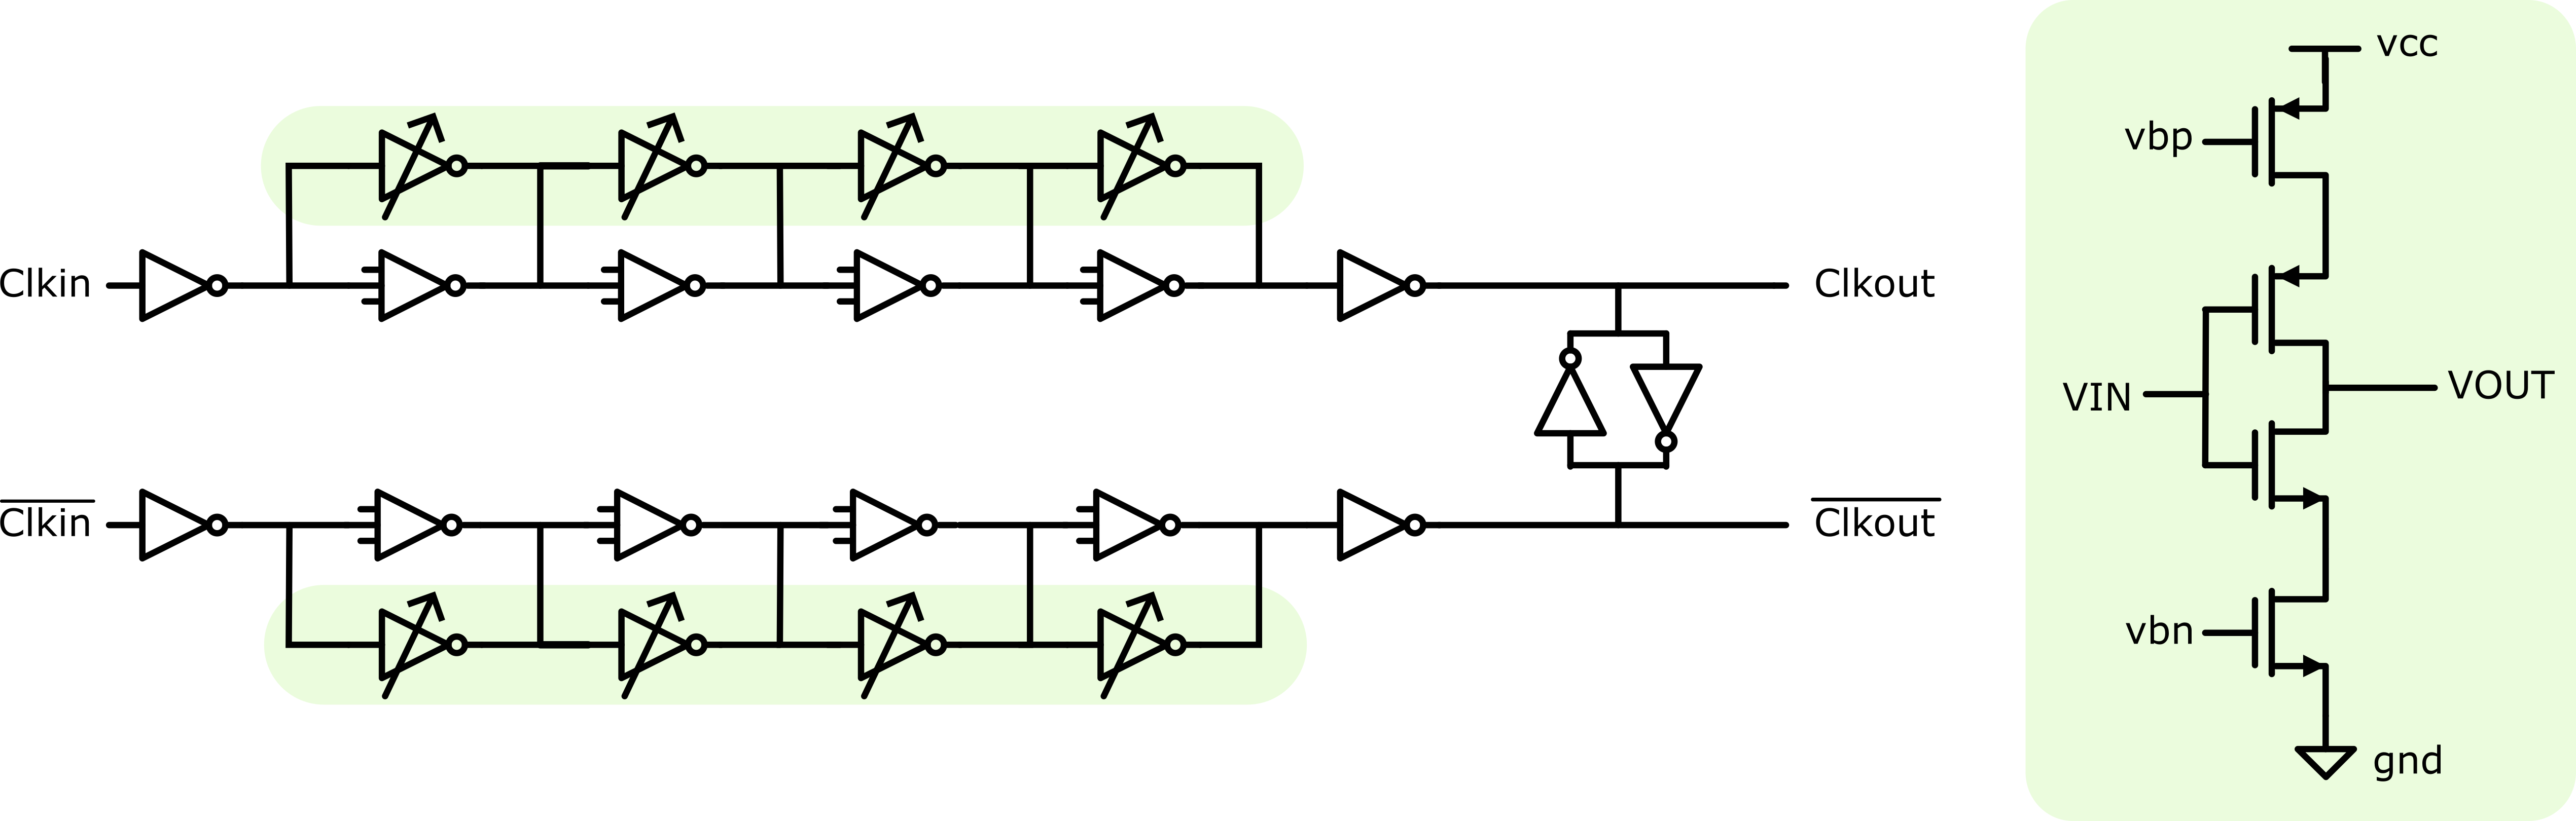
\includegraphics[width=0.8\linewidth]{figures/Schematics/old_chain.png}
  \caption{Current-starved delay stage with programmable inverters.}
  \label{fig:current_starved_delay_stage}
\end{figure}

The delay is controlled by modulating the gate voltage of the pull-up and pull-down transistors within the current-starved inverters. This bias voltage is generated by an external Digital-to-Analog Converter (DAC), as shown in Figure \ref{fig:current_starved_dac}, which limits the charging and discharging current at the inverter's output node. By adjusting this current, the rise and fall times of the output signal are controlled, thereby adjusting the delay.

\begin{figure}[H]
  \centering
  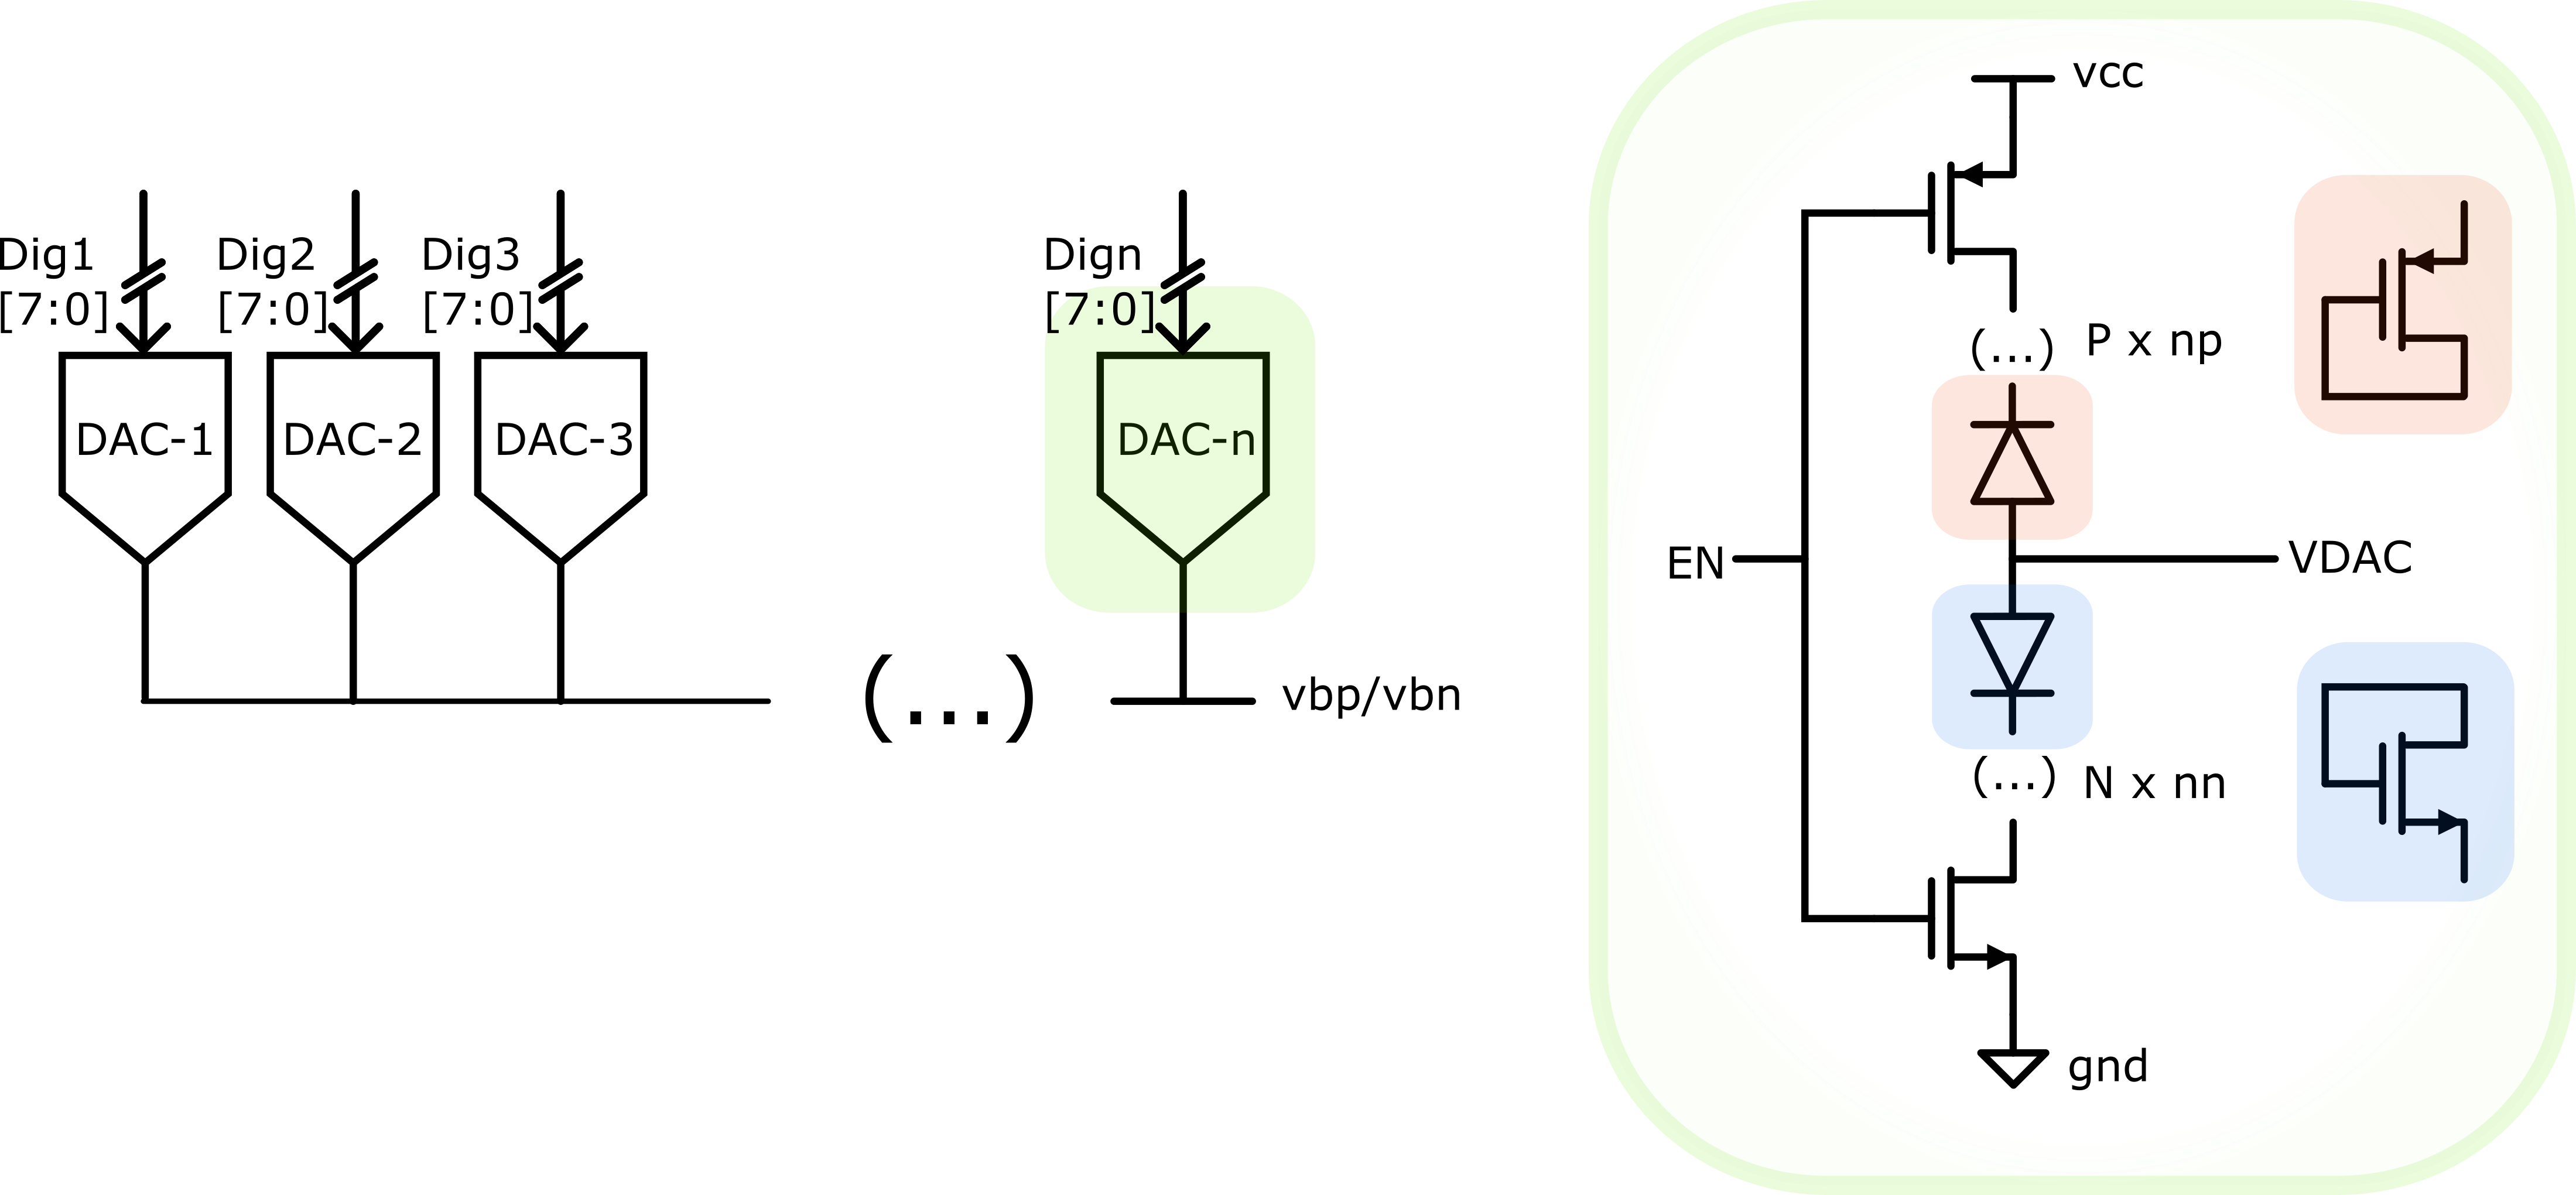
\includegraphics[width=0.8\linewidth]{figures/Schematics/old_DAC.png}
  \caption{Current-starved DAC used for biasing the current-starved inverters.}
  \label{fig:current_starved_dac}
\end{figure}

A feature of this design is that the pull-up (PMOS) and pull-down (NMOS) branches of each current-starved inverter are individually addressable. This allows for independent control over the rising and falling signal edges, providing a mechanism for duty-cycle correction.

The control DACs for the current-starved inverters are implemented using diode-based DACs. Structurally, each DAC resembles an inverter, with an enable (EN) signal controlling an NMOS and PMOS pair. The path between the drains of the input transistors and the output is connected to a series of diodes. The number of diodes is inversely proportional to the strength of the corresponding pull-up or pull-down branch. For example, a DAC with eight diodes in the pull-up path and one in the pull-down path will have a significantly stronger pull-down capability. Multiple DACs are connected to a common output node, and their cumulative effect determines the final bias voltage. Enabling more DACs with a bias towards higher or lower voltages pulls the output node voltage up or down accordingly, which in turn modulates the gate voltage of the current-starved inverters and adjusts the maximum pull-up and pull-down current of the inverter(s), modulating the delay.

A simple examination of this design highlighted an INL with a maximum error of approximately 20~LSB across the full range of the DAC (see Figure~\ref{fig:current_starved_dac_inl}). The delay range under typical operating conditions was approximately 7.6~ps (Figure \ref{fig:current_starved_dac_delay_range}). Assuming a completely linear response, since the DAC provided 256 codes, the minimum delay step was approximately 7.6~ps/256 = 30~fs. The resolution of this design was exceptional, but the INL and the delay across codes reveal that to achieve such fine resolution, the design would need to operate close to the middle of the full allowable range, which would greatly reduce the total range.

\begin{figure}[H]
  \begin{subfigure}{0.4\linewidth}
    \centering
    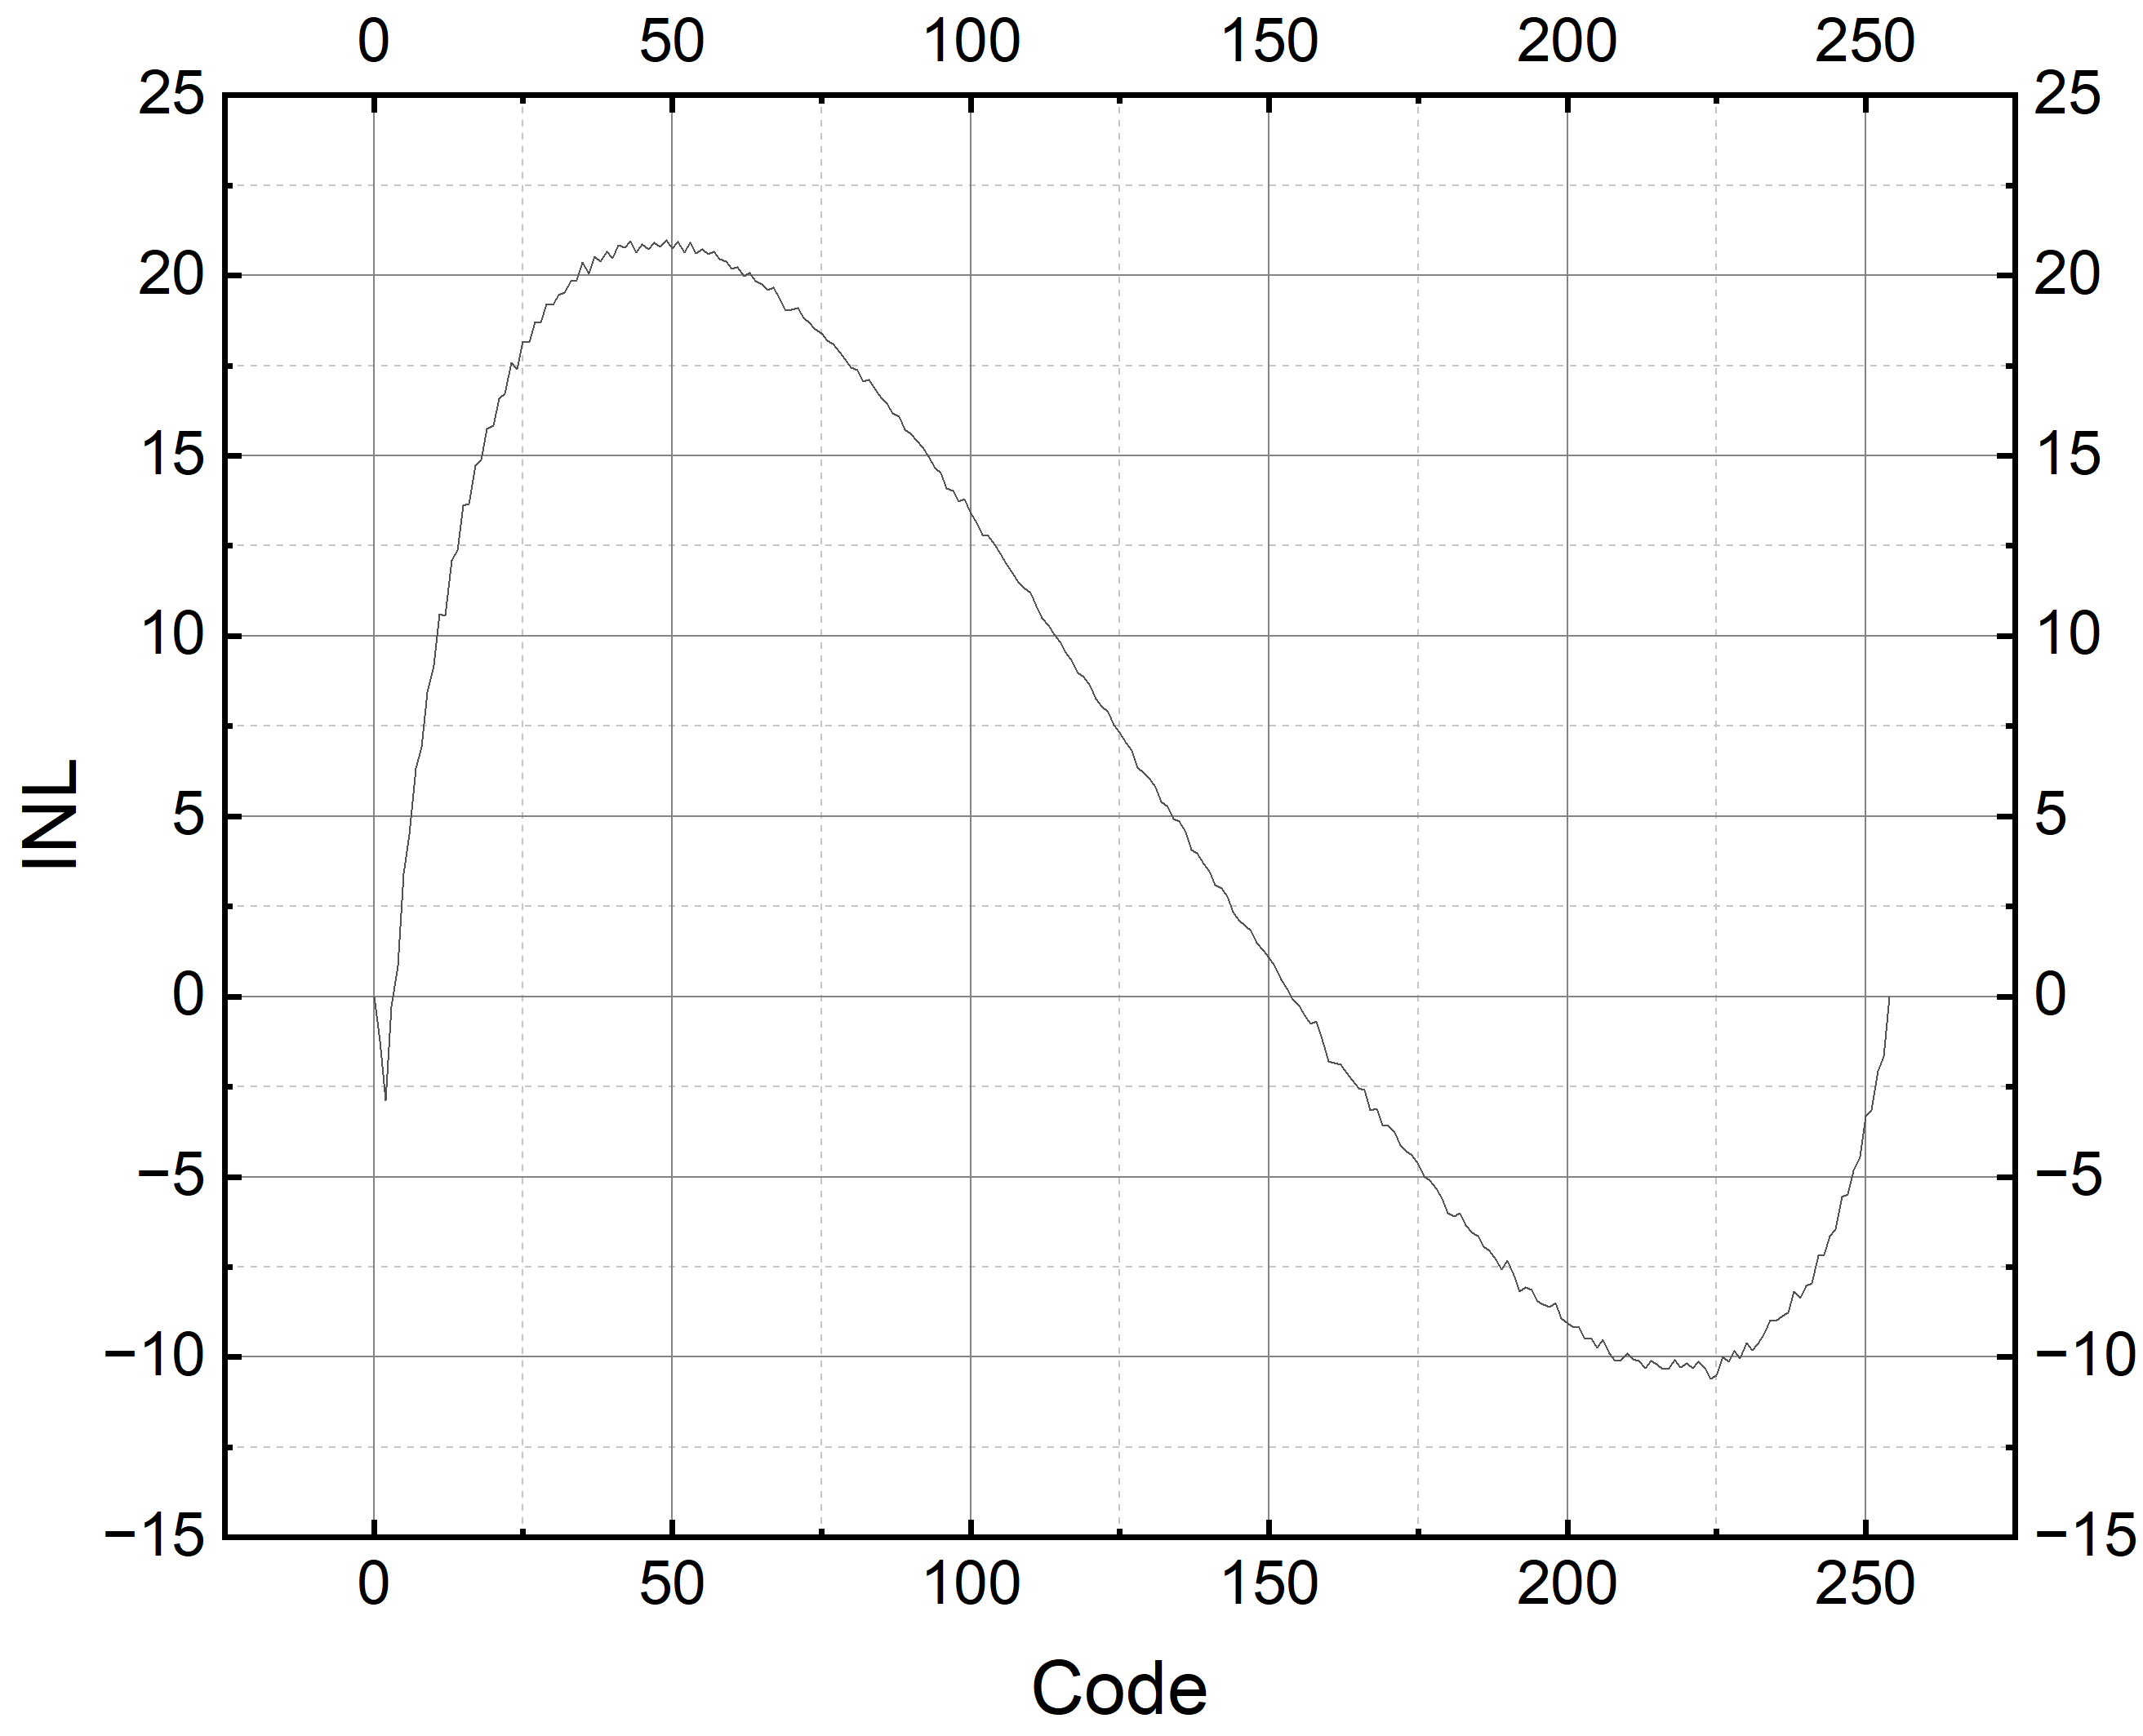
\includegraphics[width=\linewidth]{figures/Results/Previous Implementation-INL.png}
    \caption{INL of the CSI-DAC delay line.}
    \label{fig:current_starved_dac_inl}
  \end{subfigure}
  \begin{subfigure}{0.4\linewidth}
    \centering
    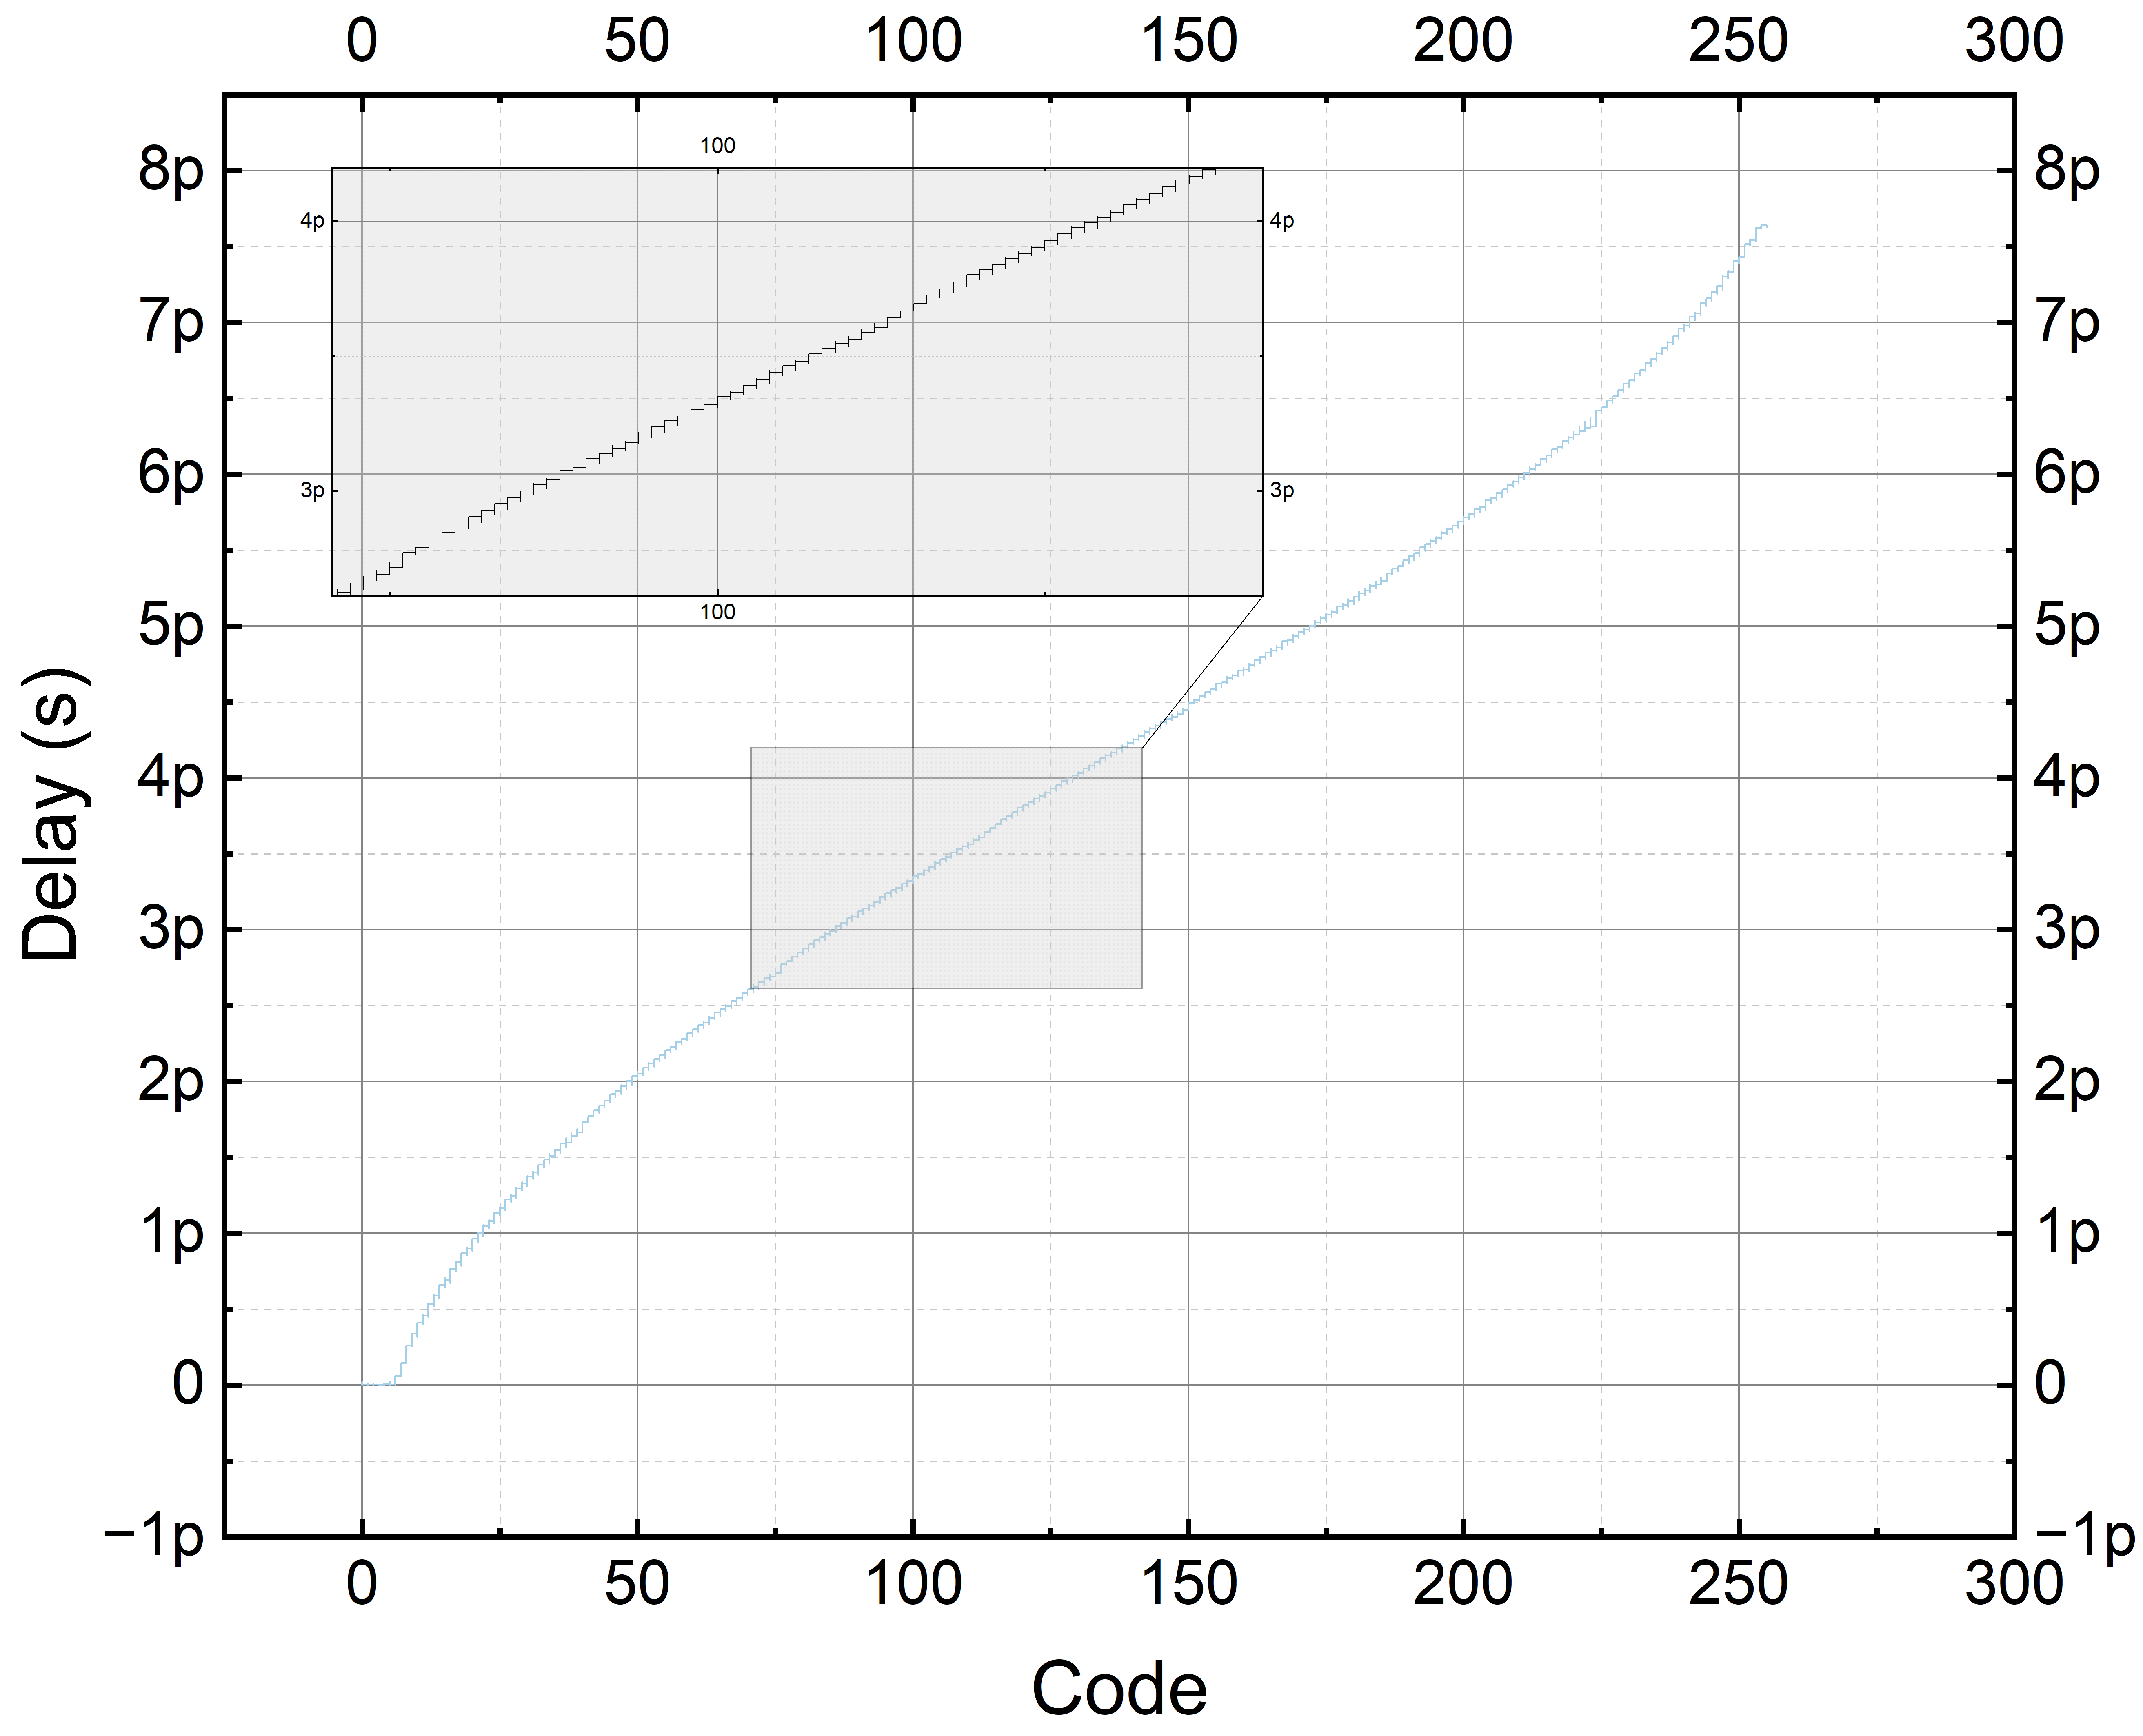
\includegraphics[width=\linewidth]{figures/Results/Previous Implementation-DelayAcrossCodesWithZoomIN.png}
    \caption{Delay across codes of the previous CSI-DAC delay line.}
    \label{fig:current_starved_dac_delay_range}
  \end{subfigure}
\caption{Characteristics of the previous current-starved delay stage implementation.}
\end{figure}

\section{Early Architectural Explorations}\label{sec:methodology}

This section details the design and verification strategies explored for the eight‑phase on‑chip clock generation and calibration circuit. The development process involved a progression from initial transistor characterization and multiple architectural iterations to the implementation of algorithm-assisted calibration loops and, ultimately, porting the design down from $7nm$ to $3nm$ and building a complete 3-path design, correctly operating at frequencies ranging from 22.5 down to 5 Gigahertz across PVT in schematic simulations.

\subsection{Switched Capacitor Delay Element}\label{sec:switched_cap}

The first implementation of the programmable delay stage was based on a switched capacitor delay element, as detailed in~\cite{Ramazanoglu2018switched}. The design consisted of an inverter chain with seven internal nodes. Two control signals, $enb_{rise}$ and $enb_{fall}$, determined whether the rising or falling edge of the clock was to be delayed.

\begin{figure}
  \centering
  
\includegraphics[width=0.7\linewidth]{figures/Schematics/switch_cap_SCI.png}
  \caption{Switched capacitor delay element with rising and falling edge modulation.}
  \label{fig:switched_cap_delay_element}
\end{figure}

To illustrate, for falling edge modulation, $enb_{fall}$ is set low. When the input signal falls, and before this transition propagates to Node 3, the falling capacitor tap switch closes and connects a capacitor to Node 1, introducing a delay. Subsequently, when Node 4 falls while Node 7 remains low, another switch closes, discharging the capacitor to ground in preparation for the next period. Rising edge modulation operates on a similar principle with different connections within the chain. Figure \ref{fig:switched_cap_charging_cap_switch} shows the capacitor tap switch closing in the allocated time slot, charging the capacitor to Node 1. A zoomed in view of N1 shows the voltage rising at two distinct rates, when the capacitor is connected to Node 1 and when it is disconnected.

\begin{figure}[H]
  \centering
  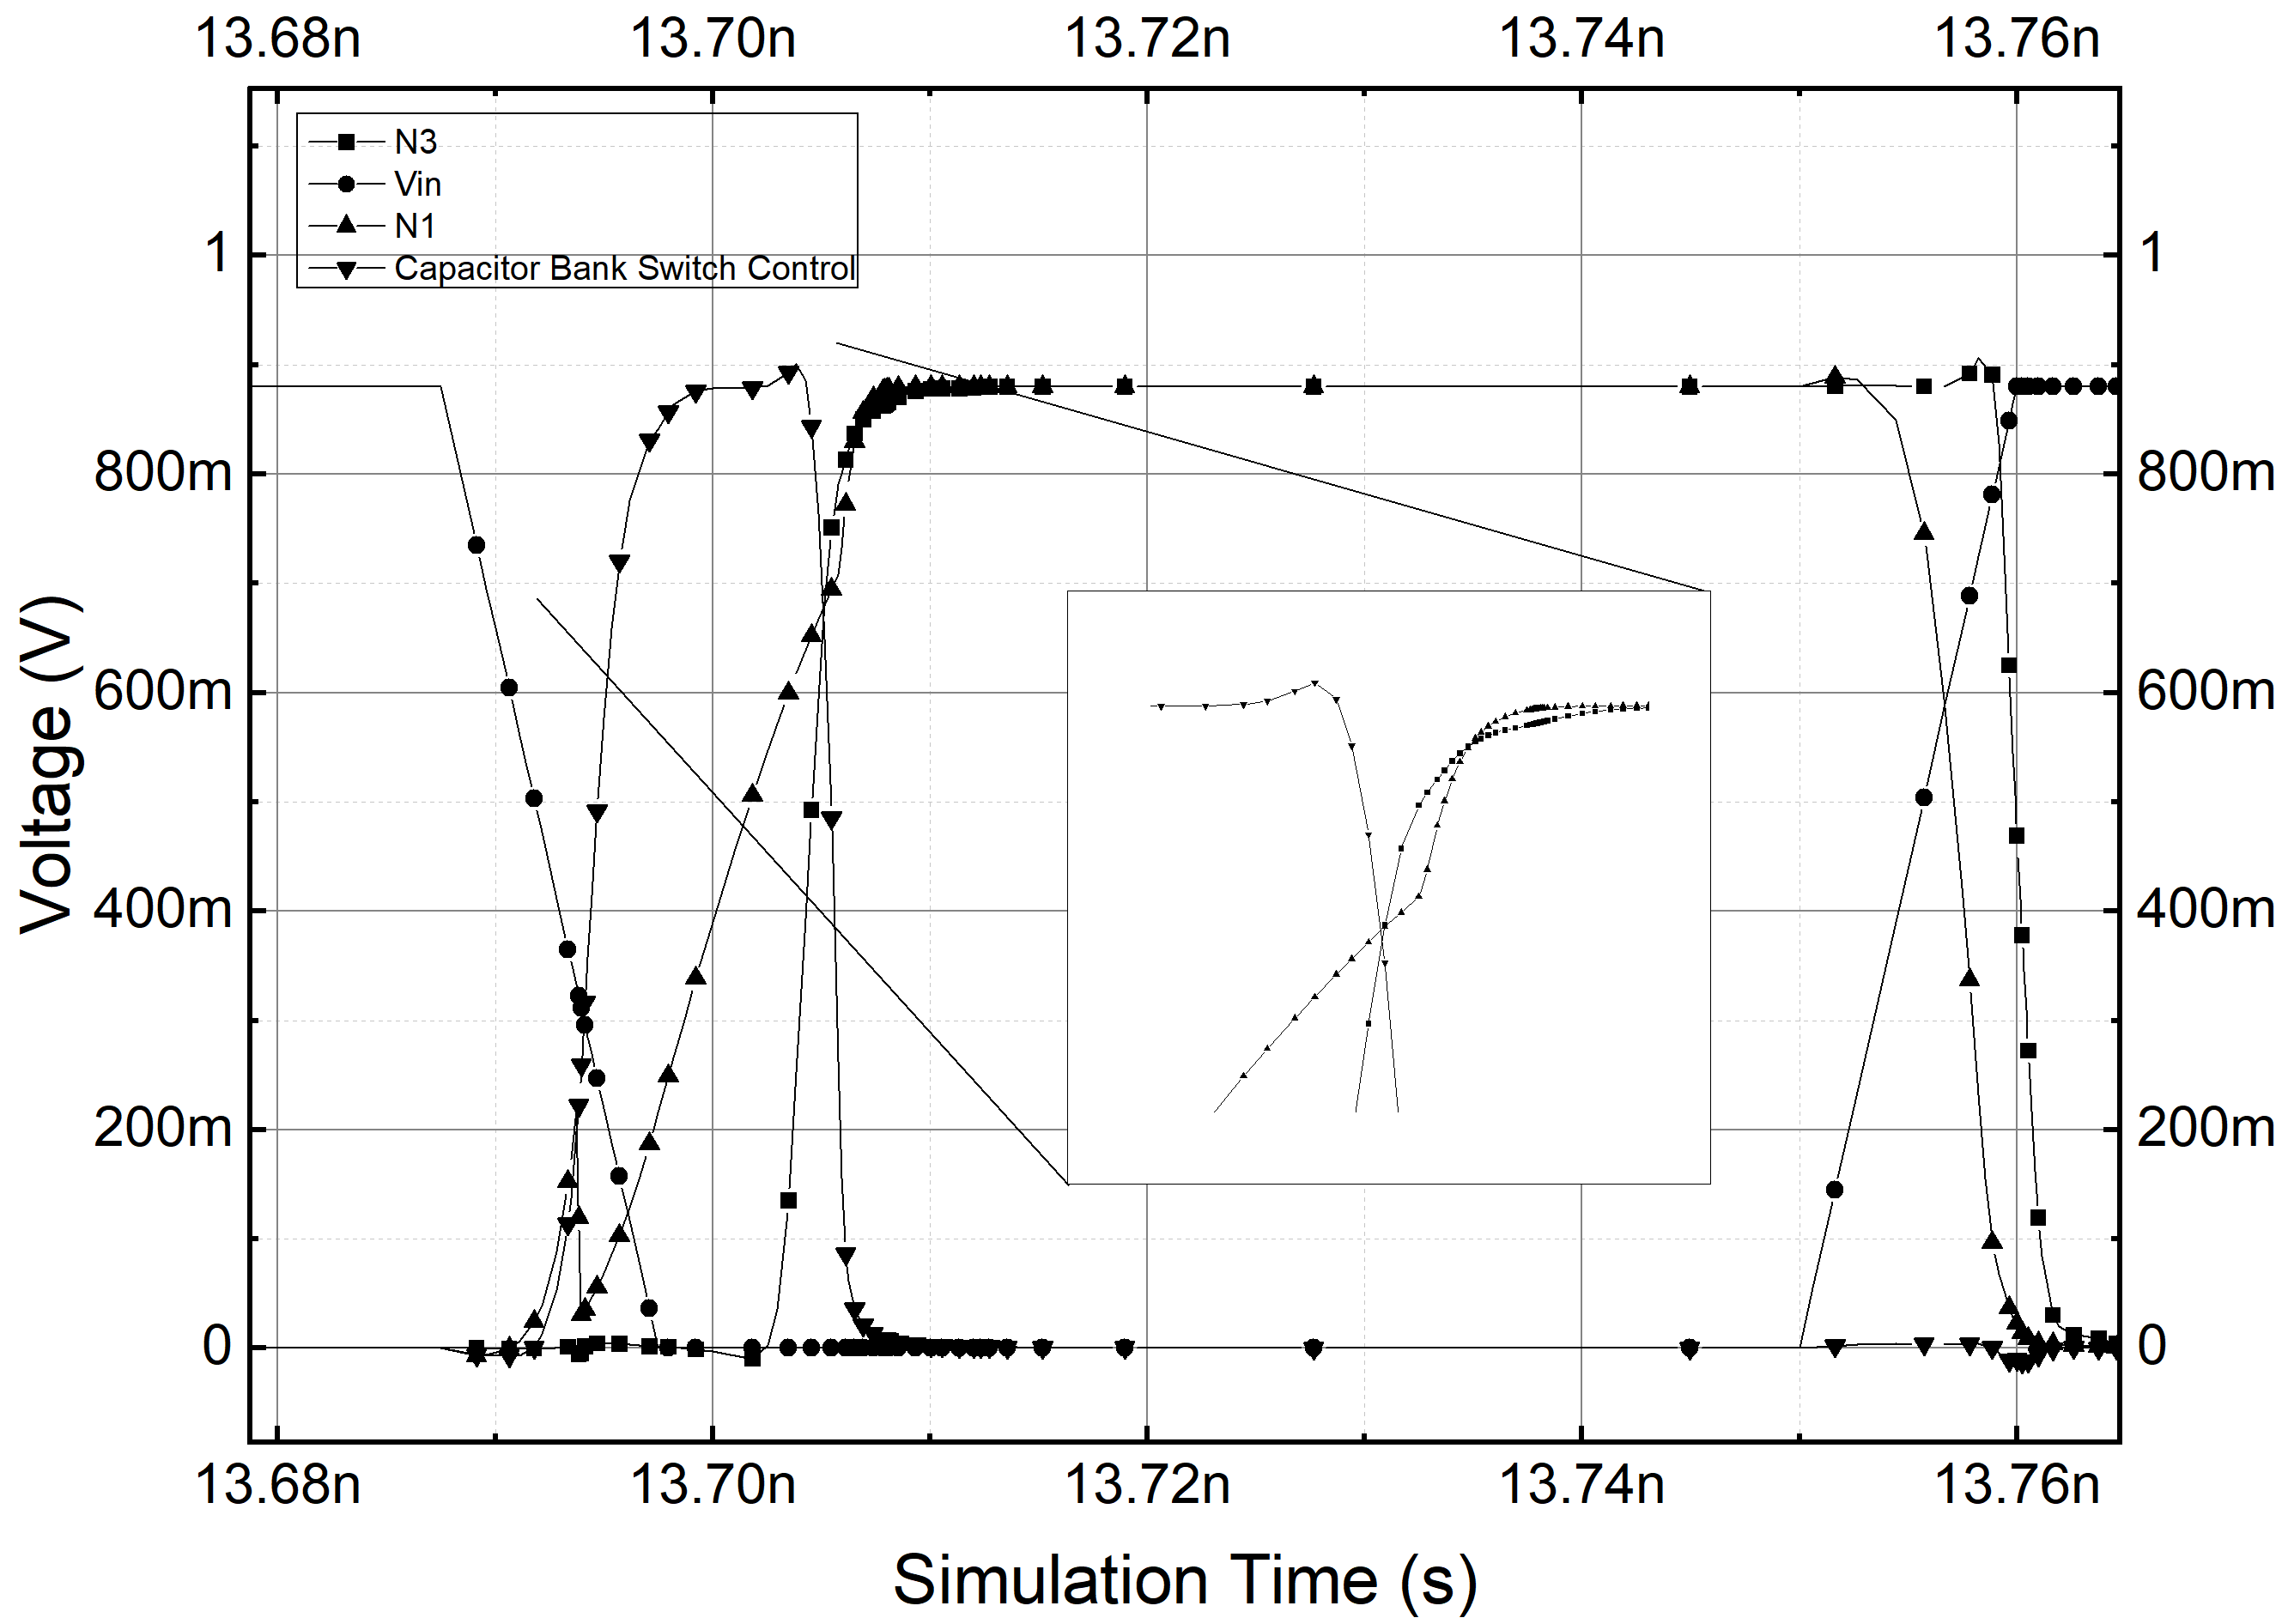
\includegraphics[width=0.5\linewidth]{figures/Results/SCI-SwitchVoltageAndLoadingTime.png}
  \caption{Switched capacitor tap switch closing and charging the capacitor to Node 1. A zoomed in view of the voltages at Node 1 shows the two distinct rates of voltage rise.}
  \label{fig:switched_cap_charging_cap_switch}
\end{figure}

This design's primary advantages are a reduction in the total capacitance required to achieve a given delay and the ability to perform duty-cycle correction using only passive elements. The circuit was simulated at \SI{8}{\giga\hertz} in a 7nm CMOS technology. Using ideal switches and a binary-weighted capacitor bank with a unit capacitance of \SI{500}{\atto\farad}, the minimum achievable delay step was approximately \SI{400}{\femto\second} (Figure \ref{fig:SCI_delayacrosscodes}). The INL plot also showed good linearity, with a maximum error of approximately 1.4 LSB across the full range of the capacitor bank.

\begin{figure}[H]
  \centering
  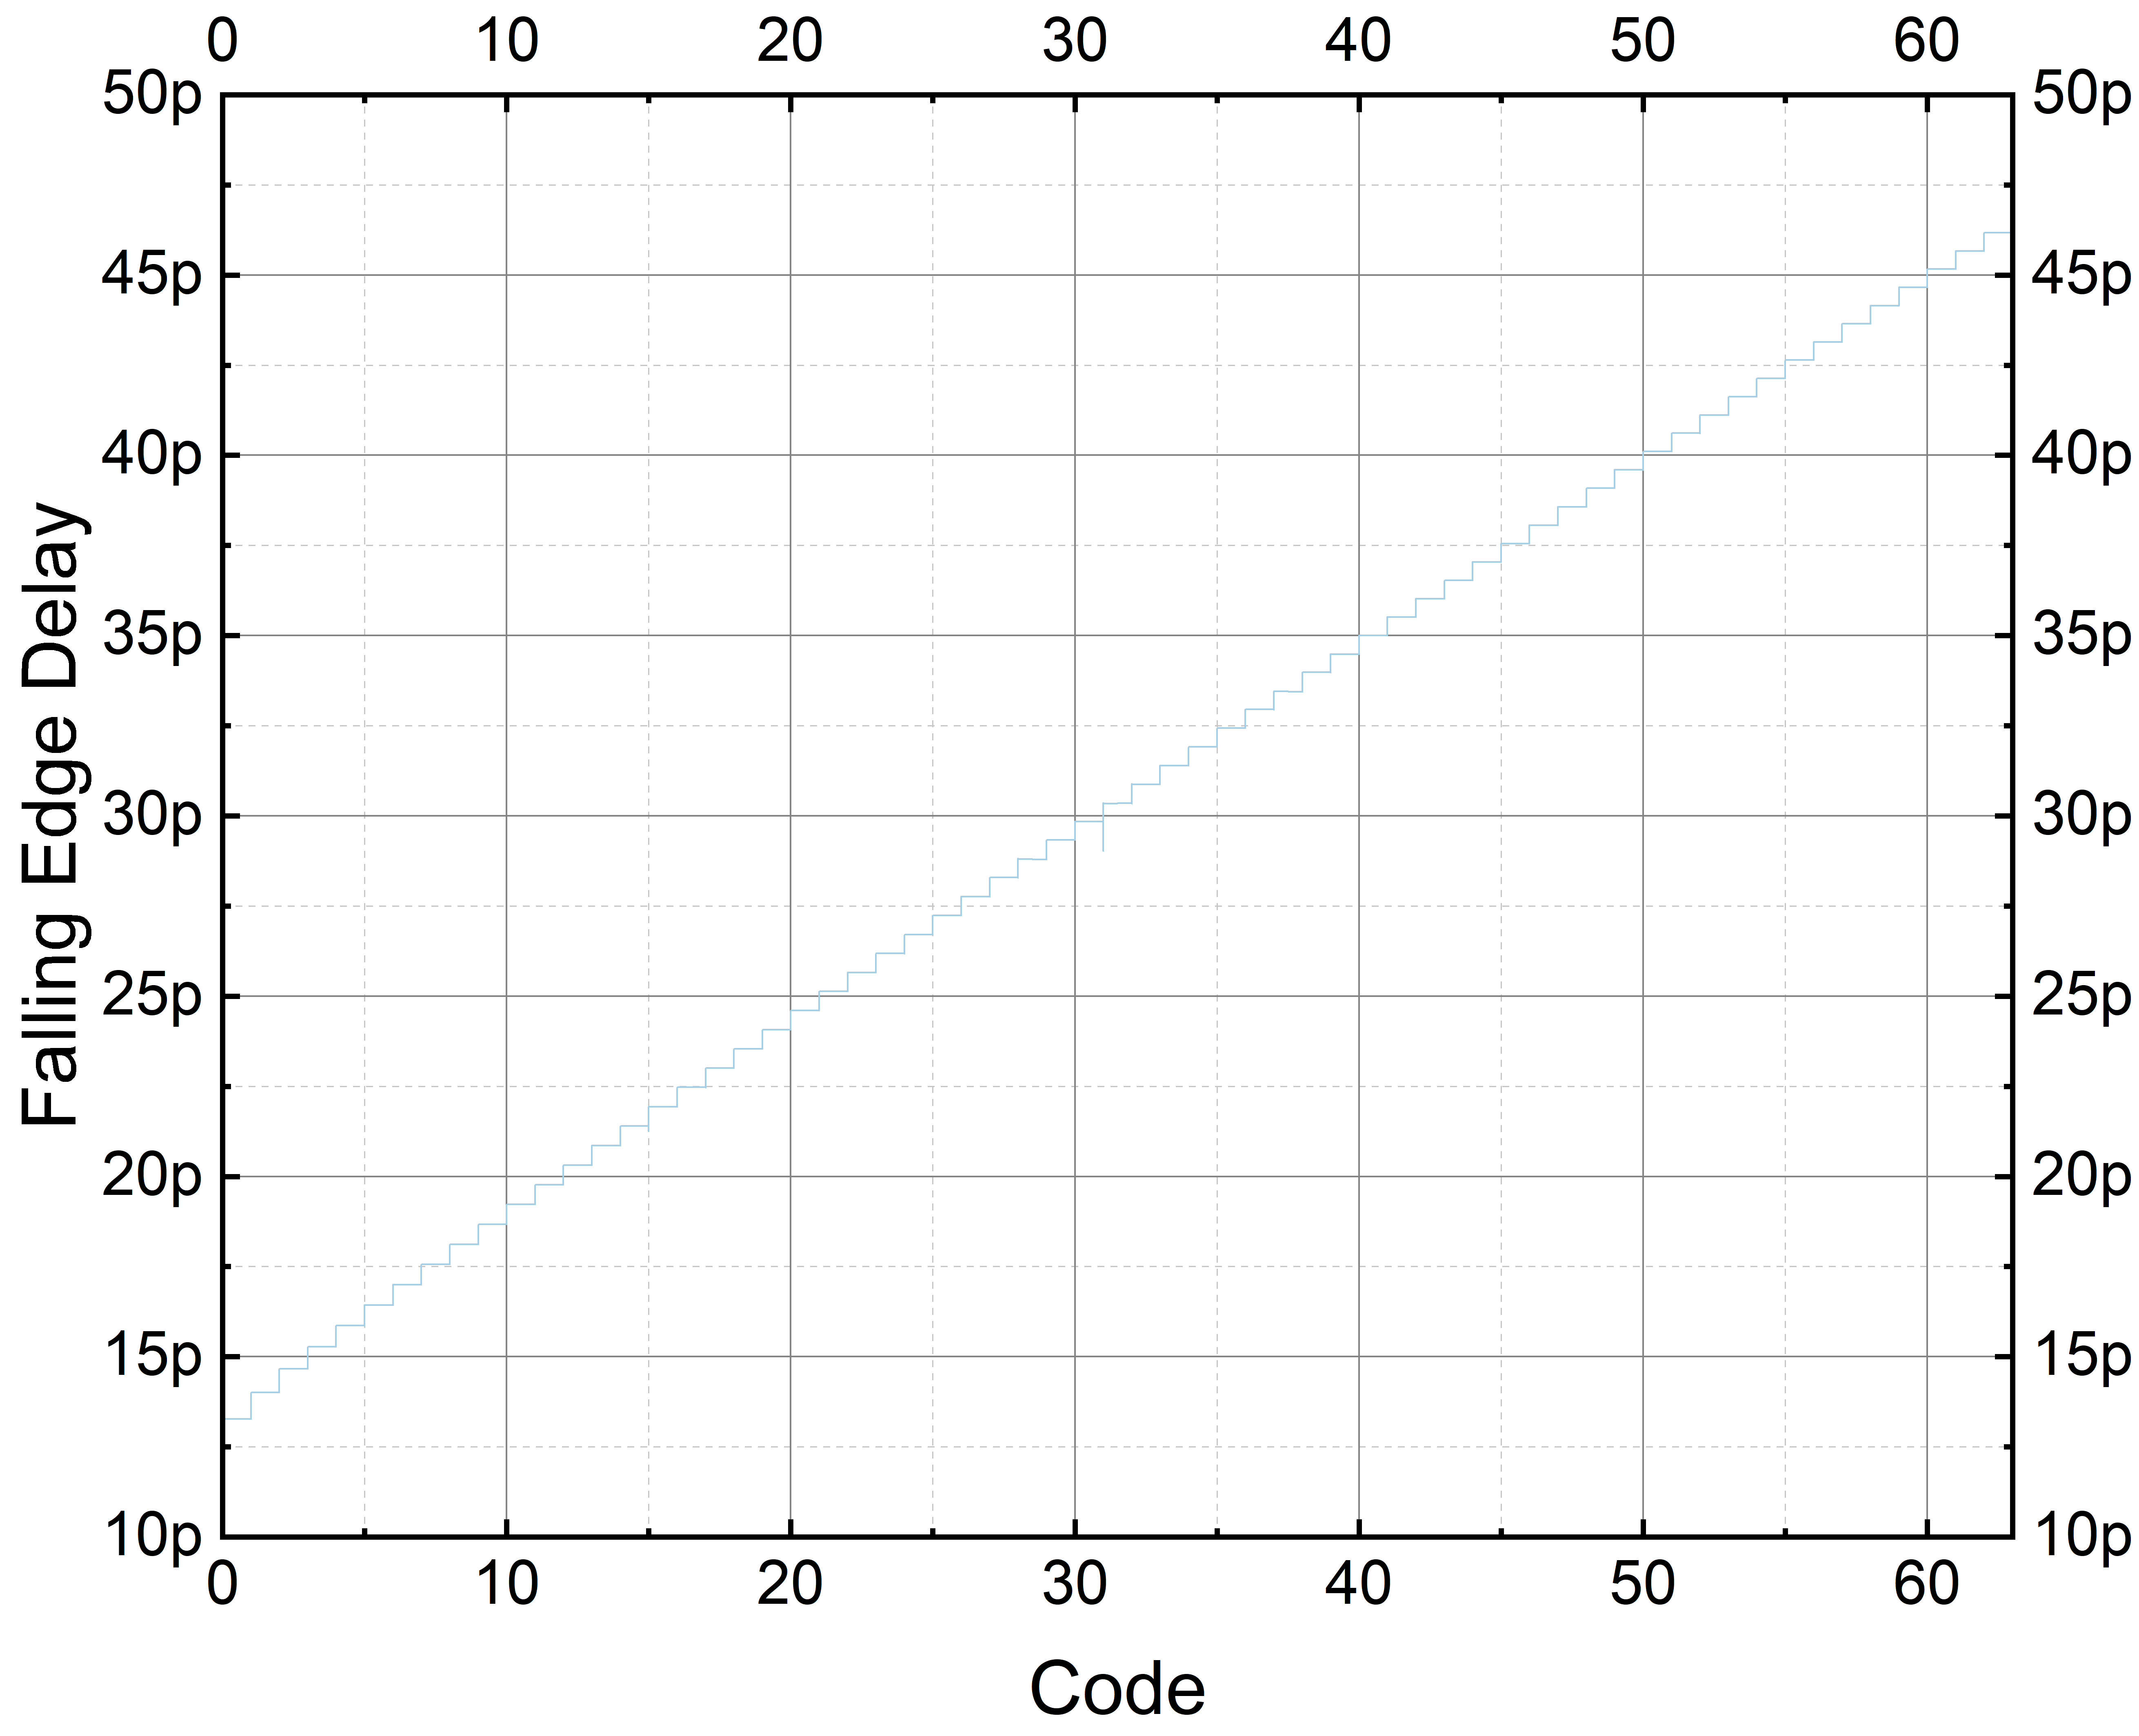
\includegraphics[width=0.5\linewidth]{figures/Results/SCI-FallingEdgeDelay.png}
  \caption{Delay across codes of the switched capacitor delay element. Codes switched across time.}
  \label{fig:SCI_delayacrosscodes}
\end{figure}

The design had, however, several limitations. The capacitor banks were large, and the design was not suitable for high-speed operation due to the complex logic and stringent timing requirements on the high-speed path. Additionally, the large area overhead of the capacitors needed for finer resolution made it impractical. Nevertheless, transient waveforms corroborated the expected behavior, and the design was verified to operate correctly at lower frequencies. 

\subsection{Phase‑Interpolator with Tunable Capacitance and Supply Biasing}\label{sec:pi_cap_supply}

Following a detailed investigation of the 7nm technology node's limitations, the target clock frequency was increased to 18GHz. The second design iteration was based on a phase-interpolator (PI) architecture, a well-established technique for multi-phase clock generation. This implementation featured two parallel paths:

\begin{enumerate}
  \item \emph{Fast Path}: A single, minimum-sized inverter contributing negligible delay.
  \item \emph{Slow Path}: Three cascaded inverters with two internal nodes ($N_1$ and $N_2$), each shunted to ground by binary-weighted MOS capacitor banks.
\end{enumerate}

The delay of the slow path was modulated by two independent control mechanisms:
\begin{description}
  \item[Capacitor Code ($C_\text{code}$)] N-bit capacitor banks at nodes $N_1$ and $N_2$ provided coarse delay tuning with steps.
  \item[Local Supply Bias ($\Delta V_\text{DD}$)] Each inverter in the slow path was powered by a controllable supply rail ($\text{AVCC}^*$), enabling fine-grained delay adjustments.
\end{description}

Refer to the schematic drawing in Figure \ref{fig:PI_1_schematic}. The fast and slow paths converge at a mixing node, $N_\text{mix}$. To ensure clean interpolation, static termination capacitors were placed on the nodes immediately preceding the mixing stage. These capacitors equalize the signal edge slopes, guiding the mixed phase toward the desired intermediate value and minimizing duty-cycle distortion (DCD).
Figure \ref{fig:PI_1_mixing_waveforms} illustrates the two mixing waveforms, one from the fast path and the other from the slow path. The slow path waveform is slightly more sinusoidal since it has been weakened by the additional capacitive load. Both waves are then mixed at the mixing node, $N_\text{mix}$, where the final phase (\ang{45} in this example) is determined by the relative strengths of the two paths. A slight duty-cycle distortion is visible in the mixed waveform, which is expected due to the unequal rising and falling edge slopes of the two paths. 
\begin{figure}
  \centering
  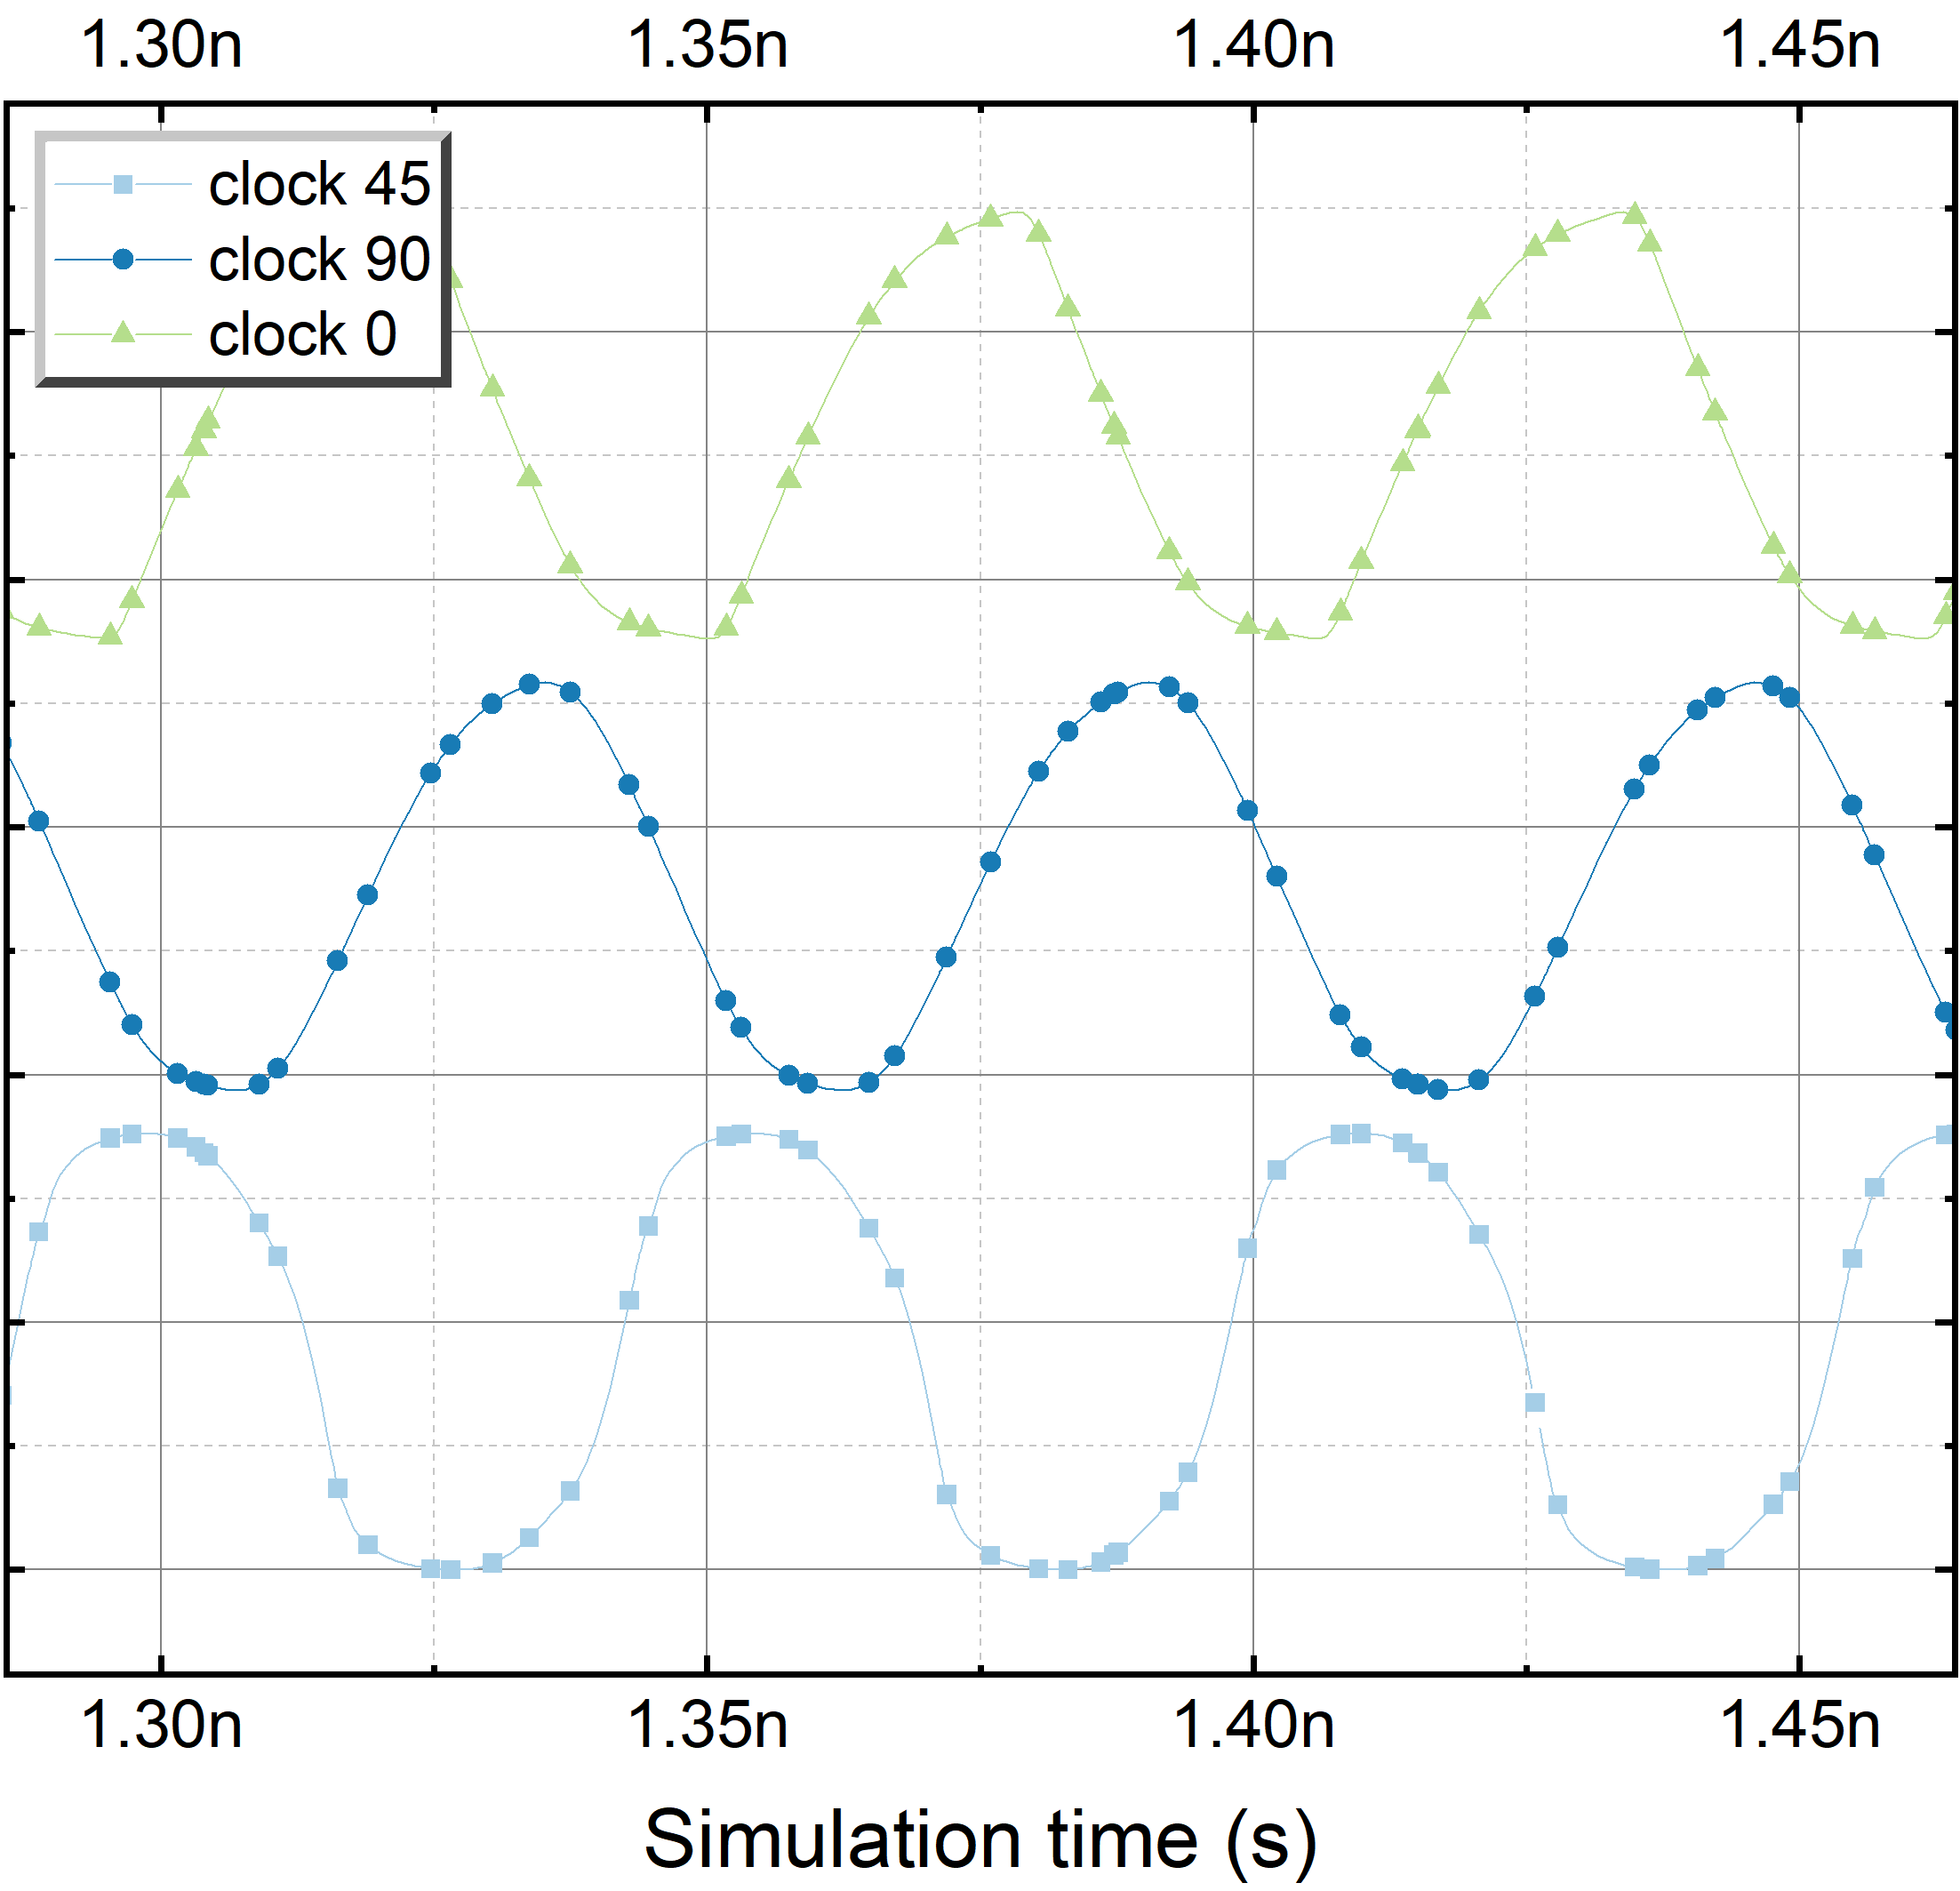
\includegraphics[width=0.5\linewidth]{figures/Results/PI_8out_CSI-clock0Clock90MixingBuildingClock45.png}
  \caption{Mixing waveforms from the fast (\ang{45}) and slow (\ang{90}) paths. The mixed waveform is the result of the two paths converging at the mixing node, \ang{45}.}
  \label{fig:PI_1_mixing_waveforms}
\end{figure}
\begin{figure}[H]
  \centering
  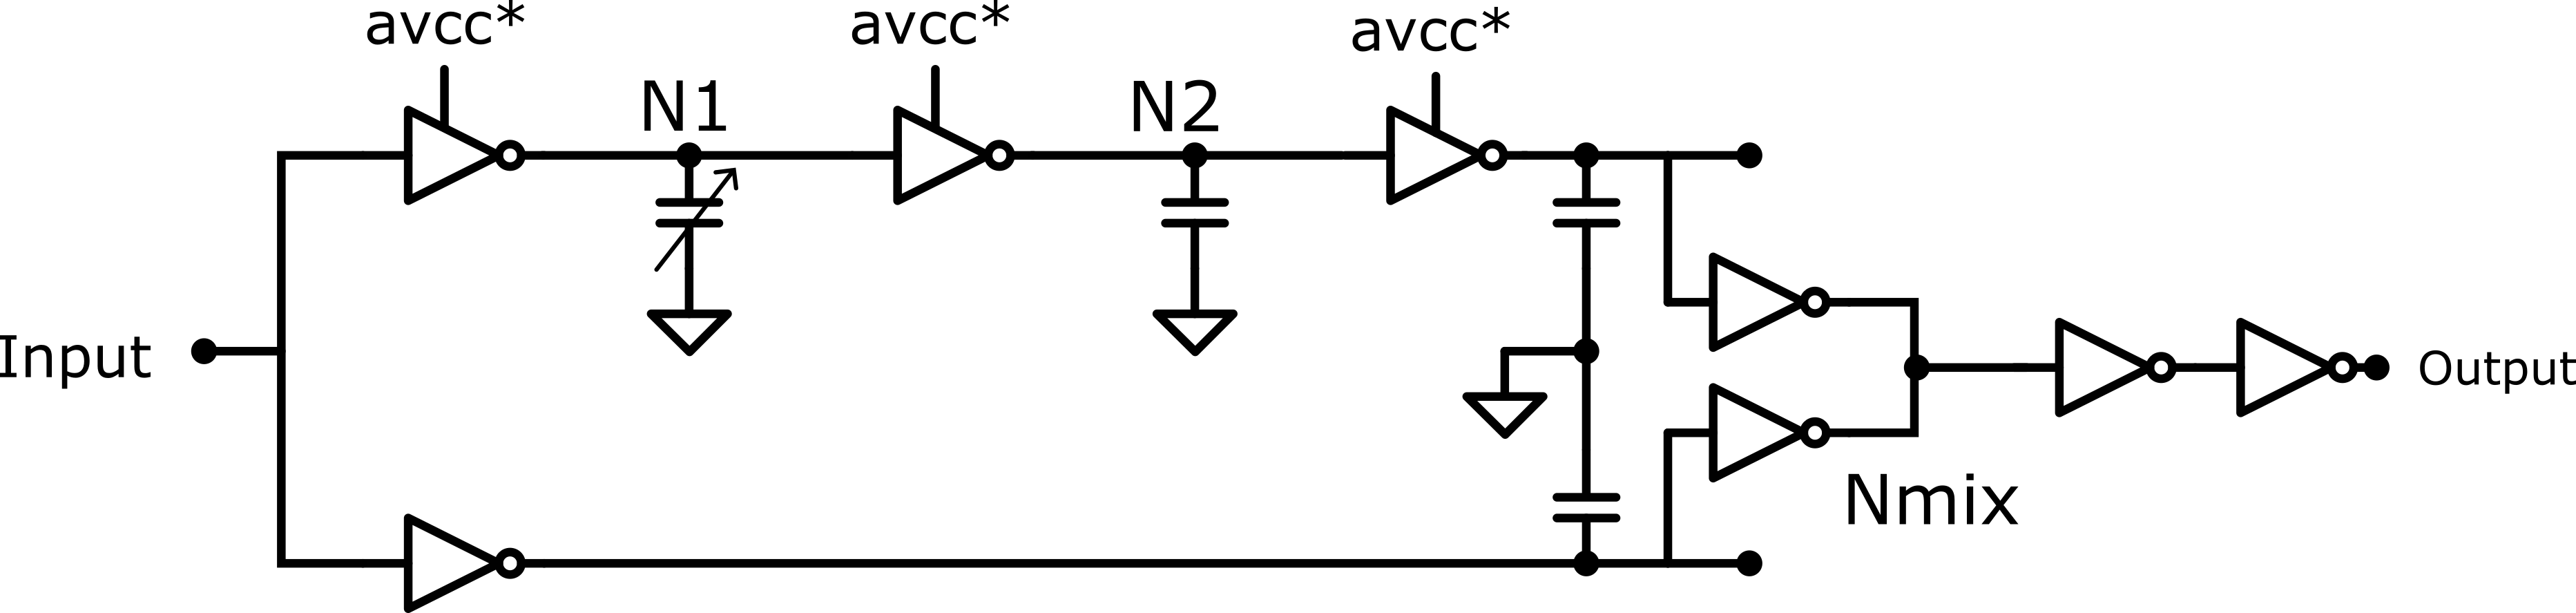
\includegraphics[width=0.8\linewidth]{figures/Schematics/clock_generation_half_V0.png}
  \caption{Phase interpolator with tunable capacitance and supply biasing.}
  \label{fig:PI_1_schematic}
\end{figure}

The resulting mixed-amplitude waveform is then passed through a final inverter, which has its own individually addressable supply, and a subsequent buffer that restores a full rail-to-rail swing, allowing for DCD correction. This final stage effectively converts the voltage/amplitude modulation into a time-domain phase shift. Assuming the threshold voltage of the last inverter is constant, a slower rising edge at the output of the avcc-tuned DCD inverter results in a delayed falling transition at the buffered output, since the threshold cross occurs later in time.
This can be easily demonstrated through the following simple equations:
%------------------------------------------------------------
% Duty‑cycle sensitivity to single‑edge slew‑rate modulation
%------------------------------------------------------------

Consider a rail‑to‑rail clock of period \(T\) and peak amplitude
\(V_{\max}\).  The decision threshold of the sampler is fixed at
\(V_{\text{th}} = V_{\max}/2\).
Denote the (approximately linear) rising‑ and falling‑edge slew
rates by \(\text{SR}_{\uparrow}\) and \(\text{SR}_{\downarrow}\), respectively:

\begin{equation}
\text{SR}_{\uparrow} \;=\;
\left.\frac{\mathrm{d}V}{\mathrm{d}t}\right|_{\text{rising}},
\qquad
\text{SR}_{\downarrow} \;=\;
\left.\frac{\mathrm{d}V}{\mathrm{d}t}\right|_{\text{falling}}.
\label{eq:slew_def}
\end{equation}

%------------------------------------------------------------
\textbf{Threshold‑crossing instants:}

Starting the rising edge at \(t=0\) and the falling edge at
\(t = T/2\), the threshold‑crossing times are

\begin{subequations}\label{eq:t_cross}
\begin{align}
t_{\uparrow}   &= \frac{V_{\max}}{2\,\text{SR}_{\uparrow}},
\label{eq:t_up} \\[2pt]
t_{\downarrow} &= \frac{T}{2} \;+\;
                 \frac{V_{\max}}{2\,\text{SR}_{\downarrow}}.
\label{eq:t_down}
\end{align}
\end{subequations}

Hence the high‑level interval measured by the sampler equals

\begin{equation}
T_{\text{high}}
    = t_{\downarrow} - t_{\uparrow}
    = \frac{T}{2} \;+\;
      \frac{V_{\max}}{2}
      \biggl(
         \frac{1}{\text{SR}_{\downarrow}}
        -\frac{1}{\text{SR}_{\uparrow}}
      \biggr).
\end{equation}

Normalising to the period gives the observed duty‑cycle

\begin{equation}
D
  \;=\;
  \frac{T_{\text{high}}}{T}
  \;=\;
  \frac{1}{2}
  \;+\;
  \frac{V_{\max}}{2T}
  \biggl(
     \frac{1}{\text{SR}_{\downarrow}}
    -\frac{1}{\text{SR}_{\uparrow}}
  \biggr).
\label{eq:D_general}
\end{equation}

%------------------------------------------------------------
\subsubsection{Modulating a single edge:}

Assume the falling‑edge slew rate is fixed at a nominal value
\(\text{SR}_{0}\), while a control knob alters the rising‑edge
slew rate by a fractional amount \(\alpha\):

\begin{equation}
\text{SR}_{\uparrow} \;=\; \text{SR}_{0}\,(1+\alpha),
\qquad
\text{SR}_{\downarrow} \;=\; \text{SR}_{0}.
\end{equation}

Substituting in \eqref{eq:D_general} yields

\begin{equation}
D(\alpha)
  \;=\;
  \frac{1}{2}
  \;+\;
  \frac{V_{\max}}{2T\,\text{SR}_{0}}
  \,\frac{\alpha}{1+\alpha}.
\label{eq:D_rising_knob}
\end{equation}

\noindent
An analogous expression is obtained if the knob instead modulates
the falling edge; the sign of the second term simply reverses.

%------------------------------------------------------------
\textbf{Small‑signal approximation:}

For \(|\alpha|\ll 1\), expand \eqref{eq:D_rising_knob} to first order:

\begin{equation}
D(\alpha)
  \;\approx\;
  \frac{1}{2}
  \;+\;
  \frac{V_{\max}}{2T\,\text{SR}_{0}}\;\alpha.
\label{eq:D_small_signal}
\end{equation}

Equation~\eqref{eq:D_small_signal} quantifies the duty‑cycle
sensitivity to a local mismatch in edge slew rate.  A
\SI{1}{\percent} increase in the rising‑edge slope therefore shifts the
duty cycle by
\(\tfrac{V_{\max}}{2T\,\text{SR}_{0}}\times\SI{1}{\percent}\).


% End of snippet

Similarly, a digital control is capable of modulating the total delay by changing the capacitance at the internal nodes. The equations that govern the delay modulation are similar to those for the duty-cycle sensitivity, with the capacitance values affecting the effective slew rates at the internal nodes. The delay can be expressed as:
For an $n$‑bit control word
$\mathbf{b}=(b_{n-1},\ldots,b_0)$, $b_i\!\in\!\{0,1\}$,
the incremental capacitance is
\[
C_{\mathrm{add}}(\mathbf{b})=\sum_{i=0}^{n-1} b_i\,C_i,
\]
yielding the effective node capacitance
\begin{equation}
C_{\mathrm{eff}}(\mathbf{b}) = C_0 + C_{\mathrm{add}}(\mathbf{b}).
\label{eq:C_eff}
\end{equation}

\subsubsection{Capacitance to edge delay:}

With pull‑up/pull‑down resistances $R_{\uparrow}$ and $R_{\downarrow}$,
the RC time constants are
$\tau_{\uparrow}=R_{\uparrow}C_{\mathrm{eff}}$ and
$\tau_{\downarrow}=R_{\downarrow}C_{\mathrm{eff}}$.
For a $50\%$ threshold the
rising and falling threshold‑crossing times become
\begin{equation}
t_{\uparrow}(\mathbf{b}) = R_{\uparrow}C_{\mathrm{eff}}(\mathbf{b})\ln 2,
\qquad
t_{\downarrow}(\mathbf{b}) = R_{\downarrow}C_{\mathrm{eff}}(\mathbf{b})\ln 2.
\label{eq:t_r_f}
\end{equation}

\textbf{Derivation of the \(\boldsymbol{\ln 2}\) factor:}

Assume a linear, time‑invariant RC network so that the step response of the
node voltage is exponential.  For the rising edge (charging through
\(R_{\uparrow}\)) we have

\[
V_\text{rise}(t) \;=\; V_{\max}\!\bigl(1-e^{-t/\tau_{\uparrow}}\bigr),
\qquad
\tau_{\uparrow}=R_{\uparrow}C_{\mathrm{eff}}.
\]

The sampler triggers when the waveform reaches one‑half of its final value,
i.e.\ when \(V_\text{rise}(t_{\uparrow})=\tfrac{1}{2}V_{\max}\).  Setting
the two expressions equal gives

\[
\frac{1}{2}V_{\max}
      \;=\;
      V_{\max}\bigl(1-e^{-t_{\uparrow}/\tau_{\uparrow}}\bigr)
\;\;\Longrightarrow\;\;
e^{-t_{\uparrow}/\tau_{\uparrow}} = \frac{1}{2}.
\]

Taking the natural logarithm of both sides,

\[
-\frac{t_{\uparrow}}{\tau_{\uparrow}}
      \;=\;
      \ln\!\Bigl(\tfrac{1}{2}\Bigr)
\;\;\Longrightarrow\;\;
t_{\uparrow}= \tau_{\uparrow}\ln 2
            = R_{\uparrow}C_{\mathrm{eff}}\ln 2.
\tag{A}
\]

For the falling edge (discharging through \(R_{\downarrow}\)) the
waveform is

\[
V_\text{fall}(t) \;=\; V_{\max}e^{-t/\tau_{\downarrow}},
\qquad
\tau_{\downarrow}=R_{\downarrow}C_{\mathrm{eff}}.
\]

The \(50\,\%\) crossing occurs when \(V_\text{fall}(t_{\downarrow}) =
\tfrac{1}{2}V_{\max}\):

\[
\frac{1}{2}V_{\max}
      \;=\;
      V_{\max}e^{-t_{\downarrow}/\tau_{\downarrow}}
\;\;\Longrightarrow\;\;
t_{\downarrow}= \tau_{\downarrow}\ln 2
              = R_{\downarrow}C_{\mathrm{eff}}\ln 2.
\tag{B}
\]

Equations \((A)\) and \((B)\) are the origin of the \(\ln 2\) factor that
appears in the timing expressions \eqref{eq:t_r_f} and consequently in the
incremental delay formulae \eqref{eq:delta_t}.

\textbf{Sampled (incremental) delay:}

Relative to a reference code $\mathbf{b}_0$,
let $\Delta C = C_{\mathrm{eff}}(\mathbf{b}) -
                C_{\mathrm{eff}}(\mathbf{b}_0)$.
Then
\begin{equation}
\Delta t_{\uparrow} = R_{\uparrow}\,\Delta C\,\ln 2,
\qquad
\Delta t_{\downarrow}= R_{\downarrow}\,\Delta C\,\ln 2.
\label{eq:delta_t}
\end{equation}

Equation\,\eqref{eq:delta_t} shows that each LSB increment of
capacitance, $C_{\mathrm{LSB}}$, introduces a fixed delay step
$R_{\uparrow(\downarrow)}\,C_{\mathrm{LSB}}\ln 2$, providing a
straight‑line transfer from digital code to timing skew.


By selecting appropriate combinations of $(C_\text{code},\Delta V_\text{DD})$, the circuit could achieve the required phase shift at the \ang{90} output. However, unequal rising and falling slew rates at the mixing node stemming from the voltage-tuning remained a significant source of error, necessitating the development of edge-balancing techniques.

\subsection{Duty-Cycle Correction and Edge-Balancing Techniques}\label{sec:dcc}

Early prototypes of the phase interpolator exhibited a duty-cycle distortion (DCD) of approximately 7\% on the slow path. The following countermeasures were evaluated to mitigate this issue:

One option was to reduce the capacitive load at node $N_2$ (the output of the final delayed inverter). This was done to more closely match its rising and falling edge rates with those of the fast path, resulting in a noticeable but insufficient improvement in DCD.

Stacked-device inverters (Figure~\ref{fig:stacked_inv}) were also explored. The standard ULVT (Ultra-Low Voltage Threshold) inverters were replaced with inverters featuring two-transistor stacked pull-up and pull-down branches. The symmetric series resistance of this stacked topology improved edge matching and significantly lowered DCD, albeit at the cost of increased device area and higher switching power. Introducing more devices into the design would also predictably increase noise and jitter, which was not acceptable for the target application, especially considering the mixing node was already a major contributor to jitter.

\begin{figure}[H]
  \centering
  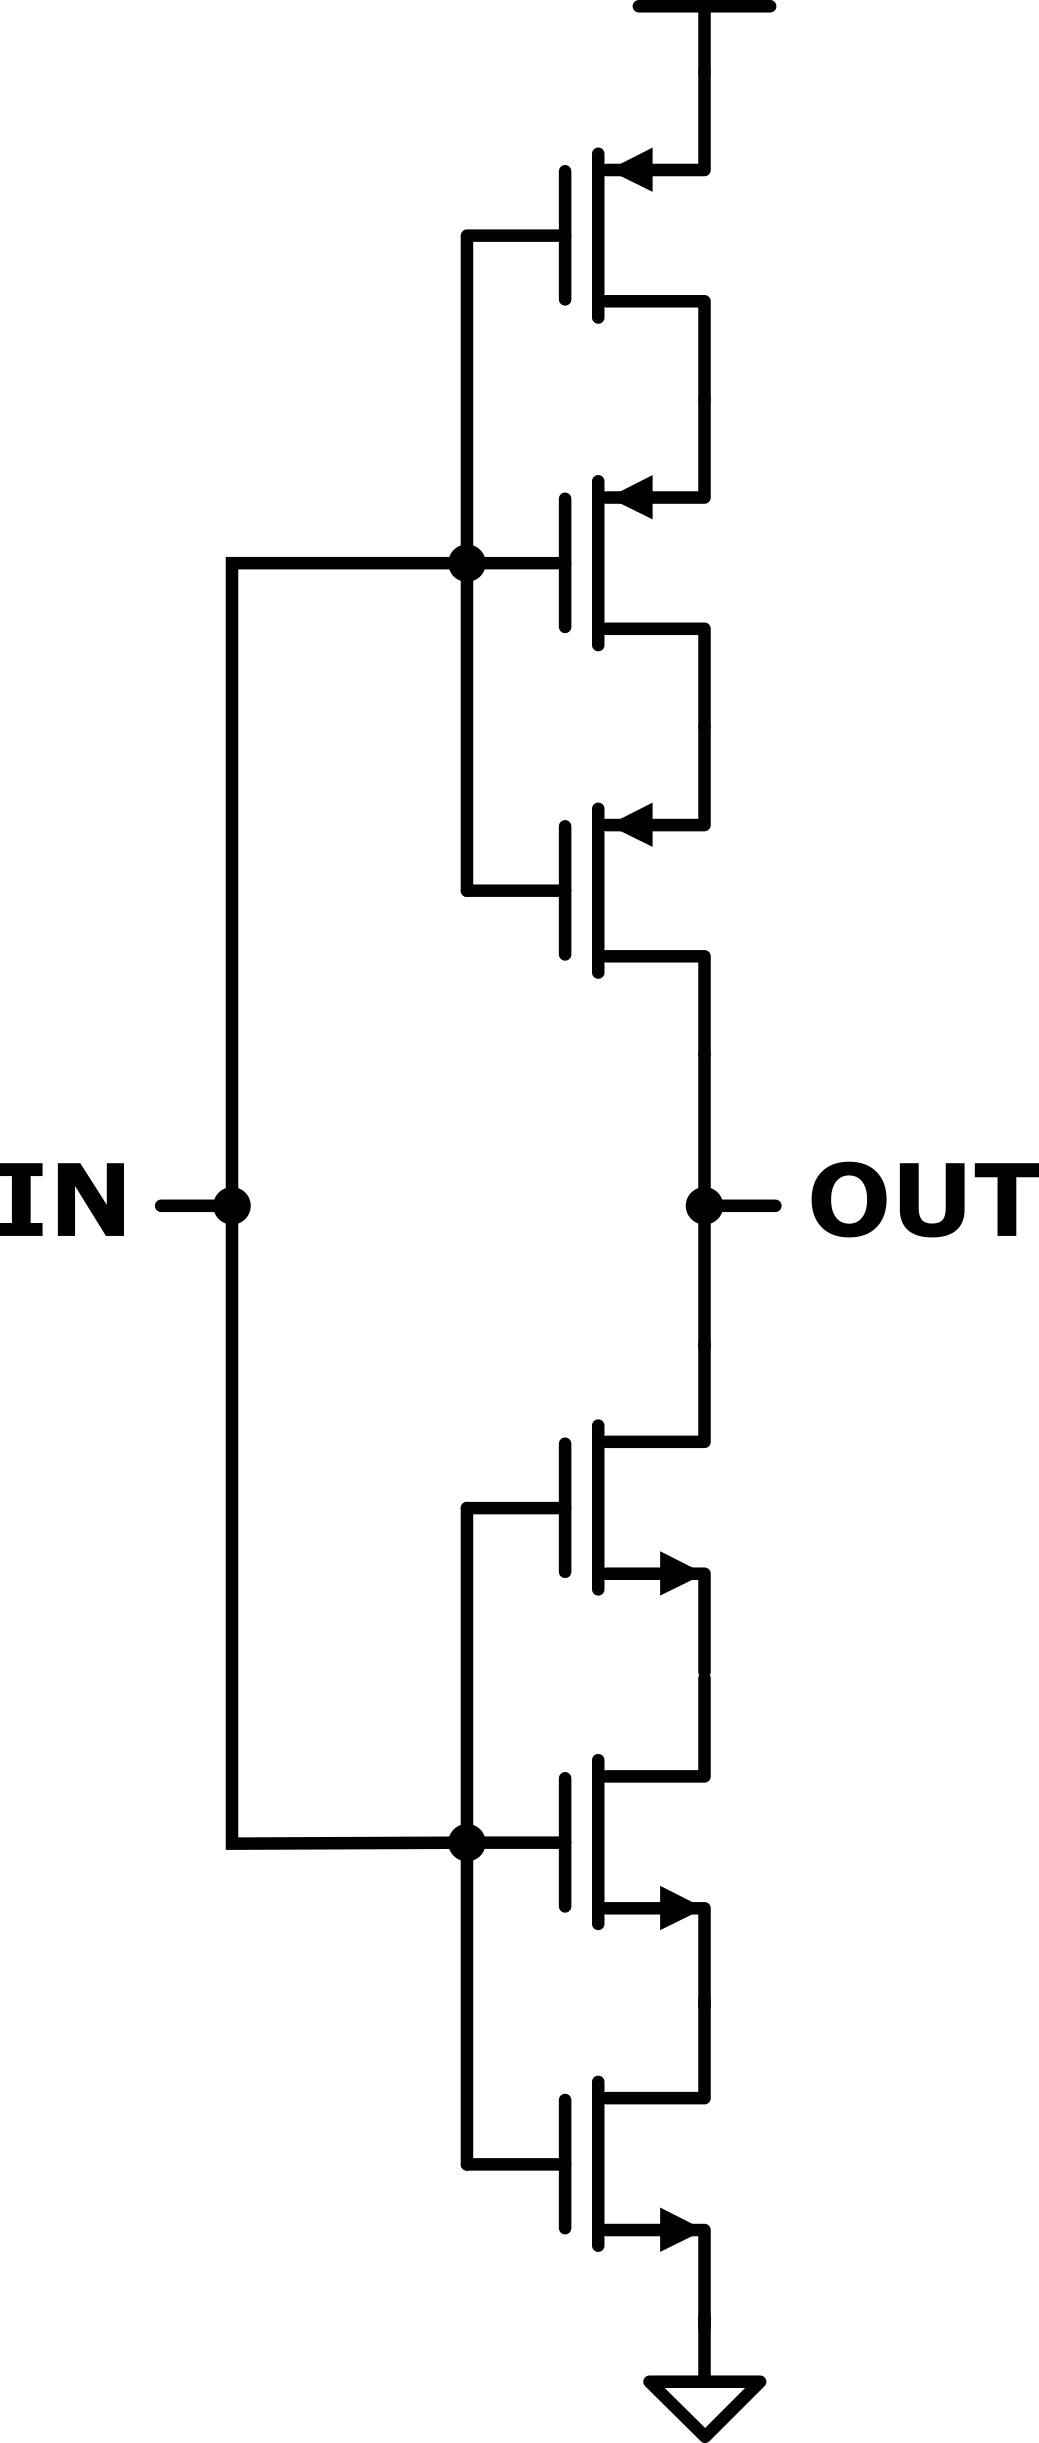
\includegraphics[width=0.3\linewidth, angle=90]{figures/Schematics/stacked_inverter-2.png}
  \caption{Stacked MOS inverter topology for edge balancing.}
  \label{fig:stacked_inv}
\end{figure}

\subsection{2-stage Supply-Bias Fine-Tuning Variant}\label{sec:avcc_finetune}

Another variant of the PI (Figure~\ref{fig:PI_2_schematic}) was developed where only the first two inverters in the delayed branch were voltage-tuned. By tuning an even number of inverters, the duty-cycle distortions induced by each stage would partially counteract one another. Key observations from this variant were that adjusting the local supply \texttt{AVCC} over a \SI{\pm45}{\milli\volt} window changed the \ang{90} phase by approximately \ang{13}, representing a significant improvement compared to the \ang{4} range of the original three-inverter tunable path. Additionally, across the same bias range, the duty-cycle distortion improved from approximately 7\% to 2\%.

These results were positive and indicated that the supply-bias fine-tuning approach could provide a means of achieving the required phase shifts with reduced DCD. However, DCD remained a concern, as it was still too high for the target application and would necessitate the addition of further correction circuitry to ensure the output clock met the stringent requirements of the SerDes system. Since jitter was a critical parameter in the overall SerDes transmission chain budget, the team decided to explore alternative methods for achieving the required phase shifts without introducing significant DCD, and possibly correcting the DCD without additional stages.

\begin{figure}[H]
  \centering
  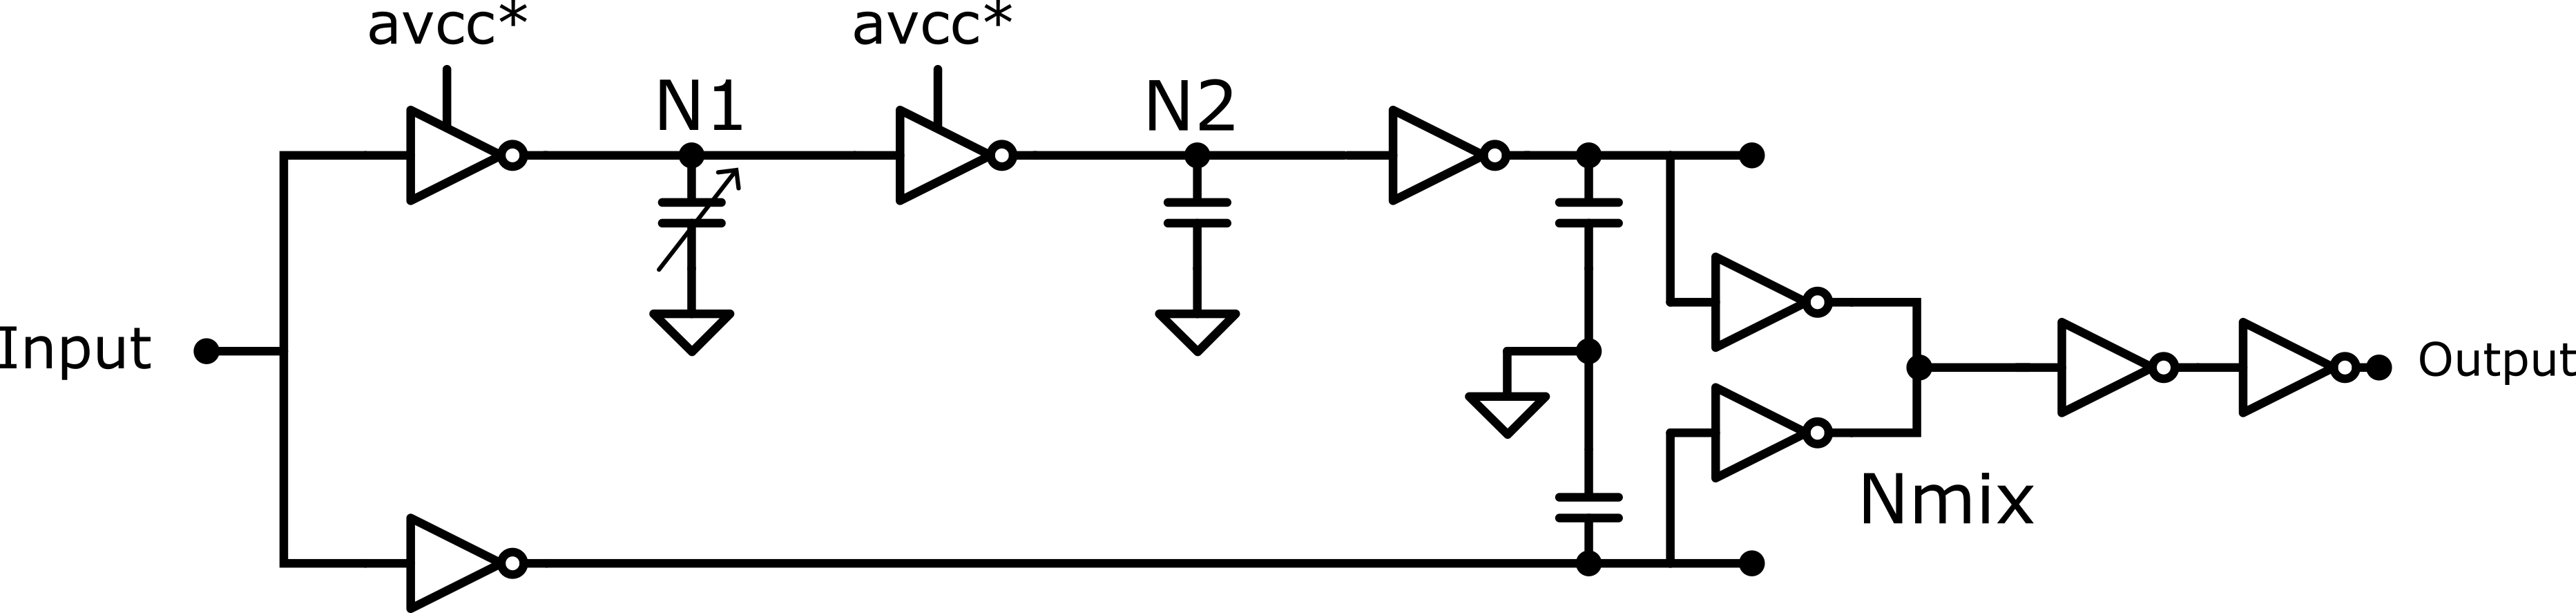
\includegraphics[width=0.8\linewidth]{figures/Schematics/clock_generation_half_V2.png}
  \caption{Phase interpolator with two-stage supply-bias fine-tuning.}
  \label{fig:PI_2_schematic}
\end{figure}

\subsection{Current‑Starved Inverter Fine Tuning}\label{sec:csi}

To decouple the fine-tuning mechanism from induced DCD, a current‑starved inverter (CSI) was reintroduced into the design (Figure~\ref{fig:PI_csi_schematic}). The CSI was placed as the second inverter in the \ang{90} branch, a location chosen because its output drives a smaller capacitive load, thereby maximizing the tuning resolution. The bias voltages $v_\text{bp}$ and $v_\text{bn}$ steer the pull‑up and pull‑down currents, respectively. A \SI{45}{\milli\volt} sweep of $v_\text{bp}$/$v_\text{bn}$, driven by a DAC with a \SI{3}{\milli\volt} step, resulted in phase shifts of \SI{35}{\femto\second} at the \ang{90} output. Critically, duty‑cycle distortion remained within 1.2\,\% across the tuning range.

\begin{figure}[H]
  \centering
  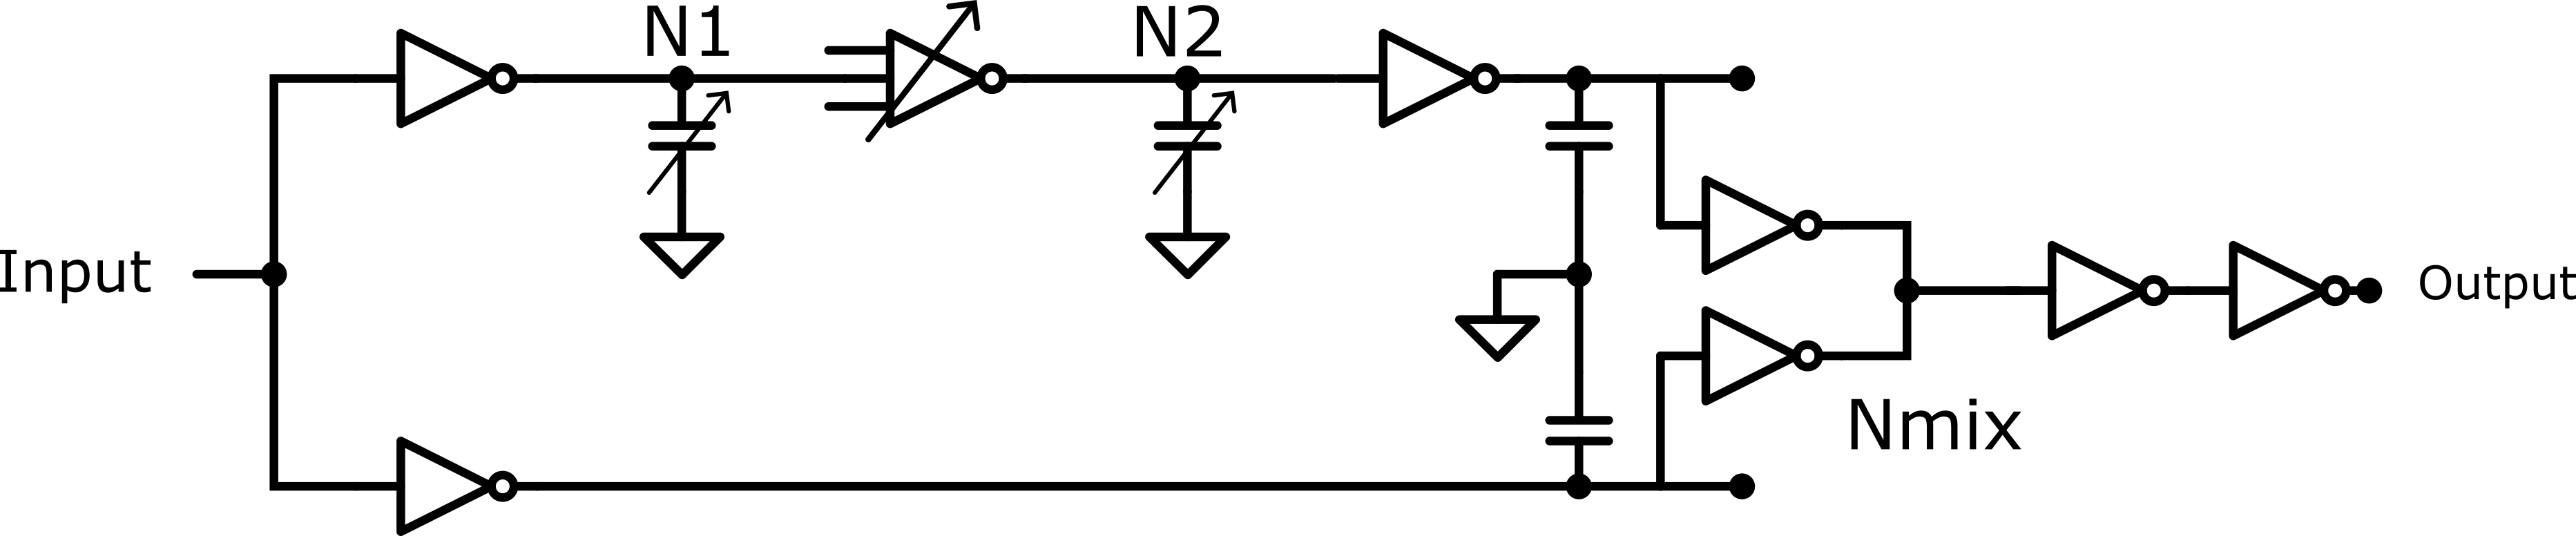
\includegraphics[width=0.8\linewidth]{figures/Schematics/clock_generation_half_CSI.png}
  \caption{Phase interpolator with current-starved inverter fine-tuning.}
  \label{fig:PI_csi_schematic}
\end{figure}

\subsection{Phase interpolation challenges and shift towards feed-forwarding}\label{sec:PI_challenges}

A fundamental challenge with phase interpolation is that it requires the rising and falling edges of the signals being mixed to be slowed down significantly. For generating a \ang{90} out-of-phase clock, the rising and falling edges must overlap sufficiently to ensure correct mixing and avoid intermediate voltage plateaus. This imposes a strict constraint on the signal rise/fall times. 

% -----------------------------------------------------------
\subsubsection{Edge‑Overlap Constraint and Its Consequences}

Phase interpolation (PI) mixes two phase‑shifted clocks, e.g.\ $0^{\circ}$ and
\ang{90}, to synthesise an intermediate phase.  To obtain a clean
rail‑to‑rail output, the rising (or falling) edges of the two inputs must
overlap long enough that the resistive (or current‑mode) summer sees
both voltages simultaneously \cite{Razavi2023PI}.  For a data‑rate (or clock)
frequency $f$ the required rise/fall time is bounded by
%
\begin{equation}
{\;
     \frac{1}{4f+t_{\text{overlap}}} 
     \;<\; t_{\text{rise}} 
     \;<\; \frac{1}{2f}
     \;}
\label{eq:overlap}
\end{equation}
%
where the designer tries to maximise $t_{\text{overlap}}$ to minimise
mid‑rail plateaus (Fig.\,\ref{fig:fast}).

\paragraph{Area penalty}:

The edge of a CMOS driver can be modelled as an \(R_{\text{on}}\)-\(C\) first‑order step.  
For the 10--90 \% definition of transition time,
\[
  t_{\text{rise}}\;\approx\;0.7\,R_{\text{on}}\,C_{\text{shunt}}.
\]
Solving for the required shunt capacitance gives  
\[
  C_{\text{shunt}} \;=\; \frac{t_{\text{rise}}}{0.7\,R_{\text{on}}}.
  \label{eq:C_shunt_area}
\]
Equation~\eqref{eq:overlap} constrains the rise time to
\(t_{\text{rise}}\gtrsim 1/(4f)\), therefore  
\[
  C_{\text{shunt}}
  \;\gtrsim\; 
  \frac{1}{\,0.7 \times 4\,f\,R_{\text{on}}}
  \;\propto\;\frac{1}{f}.
  \label{eq:C_shunt}
\]
Because a Metal–Insulator–Metal capacitor obeys \(C\propto A\varepsilon/d\),
larger \(C_{\text{shunt}}\) directly means larger layout area.  
Hence the shunt–cap block becomes the dominant footprint of the PI slice as frequency decreases. 
Since the block had to work across frequencies, tuning for a large range of frequencies would likely require large, programmable capacitors, making the design less practical.

\paragraph{Jitter}:

Figure~\ref{fig:slow} removes the mid‑rail kink but forces the waveform to
linger near the inverter’s high‑gain point.  Treat the edge as a linear ramp
of height \(\Delta V = V_{\text{DD}}\) over
\(\Delta t = t_{\text{rise}}\), so
\(dV/dt \approx V_{\text{DD}}/t_{\text{rise}}\).
Any rms voltage noise \(\sigma_v\) present at that instant is converted into
timing jitter
\[
  \sigma_t
  \;=\;
  \frac{\sigma_v}{dV/dt}
  \;=\;
  \sigma_v \,\frac{t_{\text{rise}}}{V_{\text{DD}}},
\]
which increases linearly with \(t_{\text{rise}}\)
\cite{TektronixJitterPrimer2012}.  Using the 10--90\,\% definition would simply
replace \(V_{\text{DD}}\) by \(0.8\,V_{\text{DD}}\); the scaling remains
unchanged.

\ref{eq:C_shunt} and \ref{eq:C_shunt_area} reveal that, if the design is to delay phases through slew-rate adjustments, it is disencouraged to slow down the edges more than strictly necessary, as this would increase the area and jitter.

\begin{figure}[H]
  \centering
  %------------- first sub‑figure ------------------
  \begin{subfigure}[b]{0.40\linewidth}
    \centering
    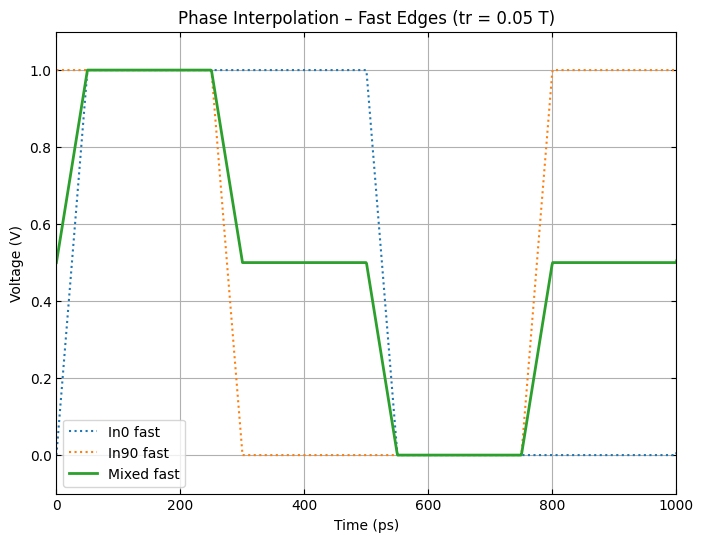
\includegraphics[width=\linewidth]{figures/Python/pi_fast_edges.png}
    \caption{Fast edges, $t_{\text{rise}}\!\ll\!1/(4f)$}
    \label{fig:fast}
  \end{subfigure}
  \hfill
  %------------- second sub‑figure -----------------
  \begin{subfigure}[b]{0.40\linewidth}
    \centering
    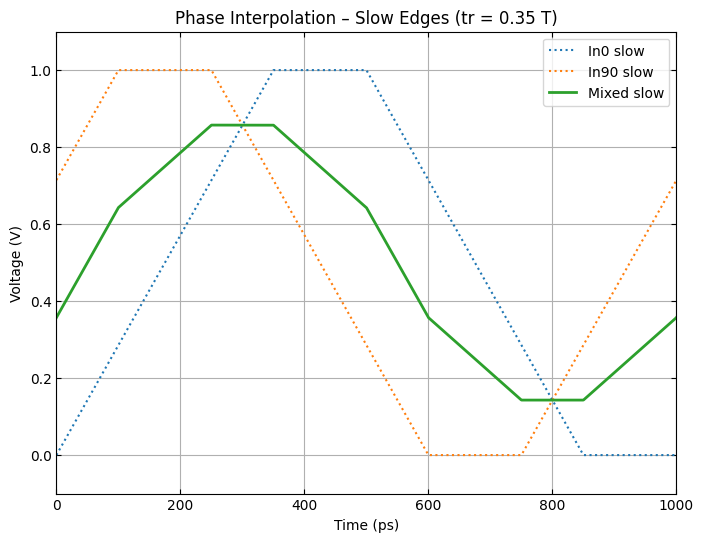
\includegraphics[width=\linewidth]{figures/Python/pi_slow_edges.png}
    \caption{Slow edges satisfying (\ref{eq:overlap})}
    \label{fig:slow}
  \end{subfigure}
  %
  \caption{Phase‑interpolator input edges and the resulting
           mid‑rail behaviour.}
  \label{fig:pi_edges}
\end{figure}
% -----------------------------------------------------------

\section{VerilogA Implementation of the tuning mechanism}\label{sec:RTL_tuning}
With some candidate circuits correctly operating at a target frequency and with specific input phase shifts and static PVT operating points, the next step was to implement a tuning mechanism that could adapt the circuit to different process corners and operating conditions and verify the ability to operate across frequencies and corners, since sweeping bias voltages and capacitances in the schematic was not practical for verification nor representative of circuit capabilities.
This way, the tuning mechanism could be tested and validated more efficiently by extracting delay step sizes, duty-cycle distortions, and other performance metrics across a range of operating conditions. Tuning dynamically during transient simulations was also important to ensure that the circuit could adapt to varying conditions without causing unintended transients or glitches in the output clock signals, which DC simulations across static control voltages could not verify.
To streamline this process, a VerilogA model of the tuning mechanism was developed. This model allowed for rapid testing and verification of the tuning logic without the overhead of full schematic simulations.


%--------------------------------------------------------------------
\subsection{Behavioural Tuning Models Implemented in Verilog-A}
\label{sec:veriloga_tuners}
%--------------------------------------------------------------------

Two fully-behavioral VerilogA blocks were written:

\begin{itemize}
  \item \textbf{\texttt{generic\_cap\_tuner}} – a switched-capacitor coarse delay tuner.
  \item \textbf{\texttt{generic\_vb\_tuner}} – a fine delay tuner that trims the propagation delay by moving the NMOS/PMOS bias voltages \texttt{VBN} and \texttt{VBP}.
\end{itemize}

Together they form a hierarchical coarse-/fine calibration loop able to absorb both process spread and temperature drift without the simulation cost of analogue parametric sweeps.

%--------------------------------------------------------------------
\subsubsection{Coarse switched–capacitor tuner (\texttt{generic\_cap\_tuner})}
%--------------------------------------------------------------------
\paragraph{Interface:}

\texttt{cap\_code[N{:}0]} drives a binary-weighted MOS capacitor bank inside the delay cell,
while \texttt{clk\_ref}, \texttt{clk\_delayed} and \texttt{enable\_tune\_pulse} are single-ended logic-level ports.
A one-shot \texttt{tune\_locked\_pulse} notifies the system controller when the block finishes.

\paragraph{Algorithm:}

Each reference-clock edge triggers a timing measurement that converts the arrival-time difference
\(\Delta t\) into a phase error
\(\varepsilon_\phi = 360^\circ \tfrac{\Delta t}{T_{\mathrm{REF}}}-\phi_\mathrm{target}\).
A proportional search then increments or decrements \texttt{cap\_code} by one LSB
until \(|\varepsilon_\phi|<\phi_\mathrm{tol,lock}\)\;(=\SI{1}{\degree}~nom.).
After every code change the tuner waits \texttt{wait\_cycles} cycles to allow analogue bias nodes to settle.
To avoid limit-cycle oscillation the code history is stored in a circular buffer; alternating up/down moves
detected over the last \texttt{history\_size} samples immediately force lock at the best recorded phase.
Optional re-tuning is enabled by the boolean \texttt{check\_for\_retune}.
If thermal drift pushes the phase outside \(\phi_\mathrm{tol,retune}\) for
\texttt{phase\_deviation\_cycles} consecutive measurements the state machine jumps back to the TUNE state.

\paragraph{Key parameters and typical values:}

\begin{center}
\begin{tabular}{@{}lrl@{}}
\toprule
Symbol & Default & Description\\
\midrule
\(\phi_\mathrm{target}\)              & \SI{270}{\degree} & Desired phase shift\\
\(\phi_\mathrm{tol,lock}\)            & \SI{0.5}{\degree} & Lock tolerance\\
\(\phi_\mathrm{tol,retune}\)          & \SI{1}{\degree}   & Retune tolerance \\[2pt]
\texttt{wait\_cycles}                 & 3                 & Dead time after each code step\\
\texttt{initial\_cap\_val}            & 0                 & Code start-up value\\
\bottomrule
\end{tabular}
\end{center}

%--------------------------------------------------------------------
\subsubsection{(Optional) Fine bias-voltage tuner (\texttt{generic\_vb\_tuner})}
%--------------------------------------------------------------------
\paragraph{Interface:}

Two analogue outputs—\texttt{vbn} (\(V_\mathrm{N bias}\)) and \texttt{vbp} (\(V_\mathrm{P bias}\))—drive current-starved inverters in the delay element.
Digital handshake pins, \texttt{tune\_locked\_pulse} and
\texttt{request\_prev\_stage\_pulse}, coordinate with the surrounding
tuning hierarchy.

\paragraph{Algorithm:}

After a rising edge on \texttt{enable\_tune\_pulse} the bias pair is reset to mid-supply.
Phase error is evaluated identically to the coarse tuner but with a
tighter lock window \(\phi_\mathrm{tol,lock}=0.1^{\circ}\).
If \(\varepsilon_\phi>0\) the module decreases \texttt{vbn} and
increases \texttt{vbp} by a fixed step \(\Delta V\)
(\SI{5}{m\volt} default), lengthening the CMOS inverter delay;
the opposite step shortens it.
When either bias reaches its limit (\texttt{vbn\_min}/\texttt{vbp\_max})
\texttt{request\_prev\_stage\_pulse} is asserted, indicating that the
preceding (coarser) element must shift its operating window.
Like its coarse counterpart the block stores a history to detect dithering and
derives a dynamic retune tolerance
\[
\phi_\mathrm{tol,retune}= \max\!\left(
                \phi_\mathrm{min},
                \alpha \cdot \Delta\!\phi_\mathrm{step@lock}
            \right)
\]
so that devices which locked with very fine steps do not trigger
unnecessary re-calibrations.

%--------------------------------------------------------------------
\subsubsection{Hierarchy and interaction}
%--------------------------------------------------------------------
Figure~\ref{fig:tuning_hierarchy} illustrates the interaction:

\begin{enumerate}
  \item All \texttt{generic\_vb\_tuner}s are pre-charged to their
        mid-values and disabled.
  \item A global pulse enables all \texttt{generic\_cap\_tuner}s.
  \item If the coarse tuner locks, it reports success via \texttt{tune\_locked\_pulse}.
  \item Vb tuner begins correction. If successful, it locks and enters a 'listening' state.
  \item If the vb tuner cannot lock, it asserts \texttt{request\_prev\_stage\_pulse} to
        the preceding coarse tuner, which then re-evaluates its phase error.
  \item The cascade continues until the phase error of every stage is within its
        fine tolerance. A final global ``all locked’’ flag is then released to the
        system clock-tree.
\end{enumerate}

This method guarantees that only one behavioural element is active at a
time, completely eliminating race conditions and analogue glitches in the clock
path, yet it converges in $\mathcal{O}(m+n)$ steps where
\(m\) and \(n\) are the coarse- and fine-resolution search spaces, respectively.

\begin{figure}[H]
  \centering
  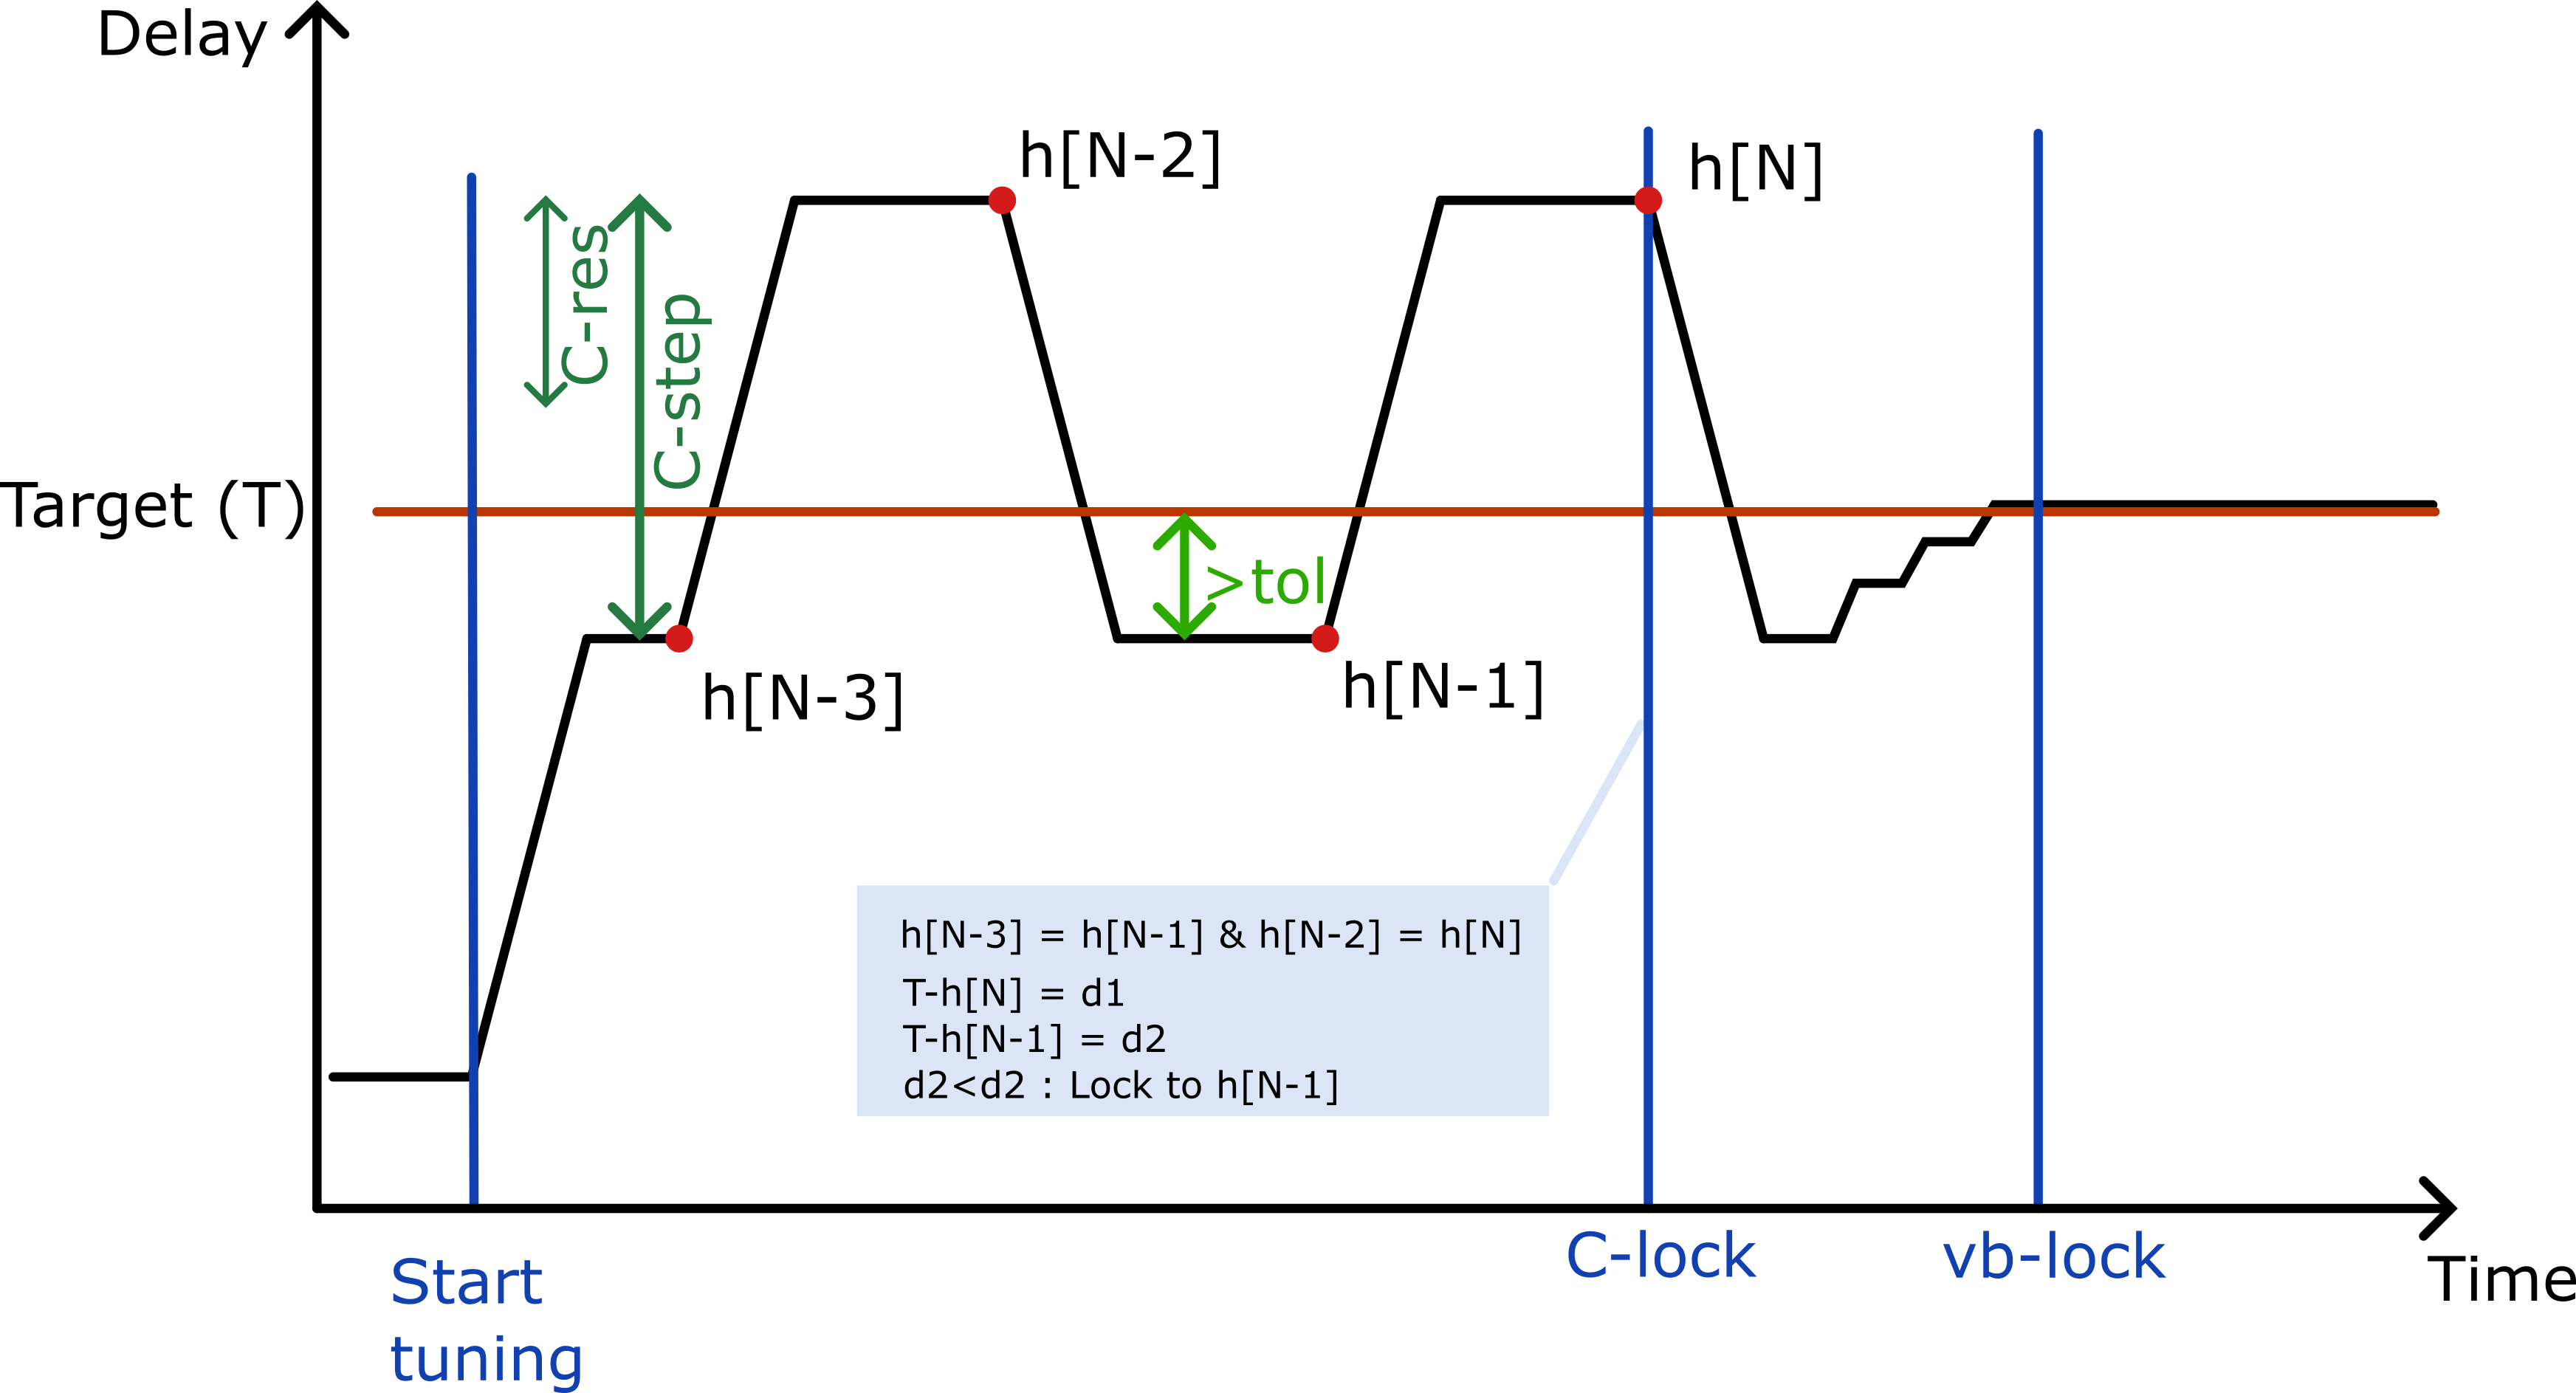
\includegraphics[width=0.8\textwidth]{figures/Schematics/Tuning_principle.png}
  \caption{Visual representation of the tuning mechanism. In this example, the coarse tuner never reaches close enough to the target phase, so it oscillates. The VerilogA block detects this, compares history samples and locks at the best phase. The fine tuner then takes over and adjusts the phase to the target value.}
  \label{fig:tuning_hierarchy}
\end{figure}


\vspace{1em}
In summary, the Verilog-A tuning infrastructure provides a fast,
self-contained and hierarchy-aware abstraction of the on-chip calibration loop,
allowing high-resolution phase characterisation over frequency, voltage and
temperature with only a fraction of the computational and time effort of schematic-level
sweeps.
%--------------------------------------------------------------------

\section{The Feed-Forward Architecture}\label{sec:feedforward}
To overcome the aforementioned limitations of phase interpolation, a new feed-forward architecture (Figure~\ref{fig:FF_half_1}) was proposed. This technique also utilizes internal nodes from two branches generating intermediate phase-shifted clocks but distinguishes itself by having a "master" and "slave" path, where the master drives an inverter that injects a current into the slave path. In other words, an internal tap from the faster signal path reinforces the slower one (or v.v.), causing the latter to settle at an intermediate phase. This method proved effective, operating with relaxed slew rate requirements at the internal nodes, making it a preferable alternative to the traditional PI design. It was stipulated that the feed-forward inverter should be programmable to allow for dynamic injection strength at the mixing node, so that both phases can be more independently controlled. As drawn in Figure~\ref{fig:FF_half_1}, the mixing occurrs before the signals are \ang{90} out of phase, relaxing the slew rate requirements.

\begin{figure}[H]
  \centering
  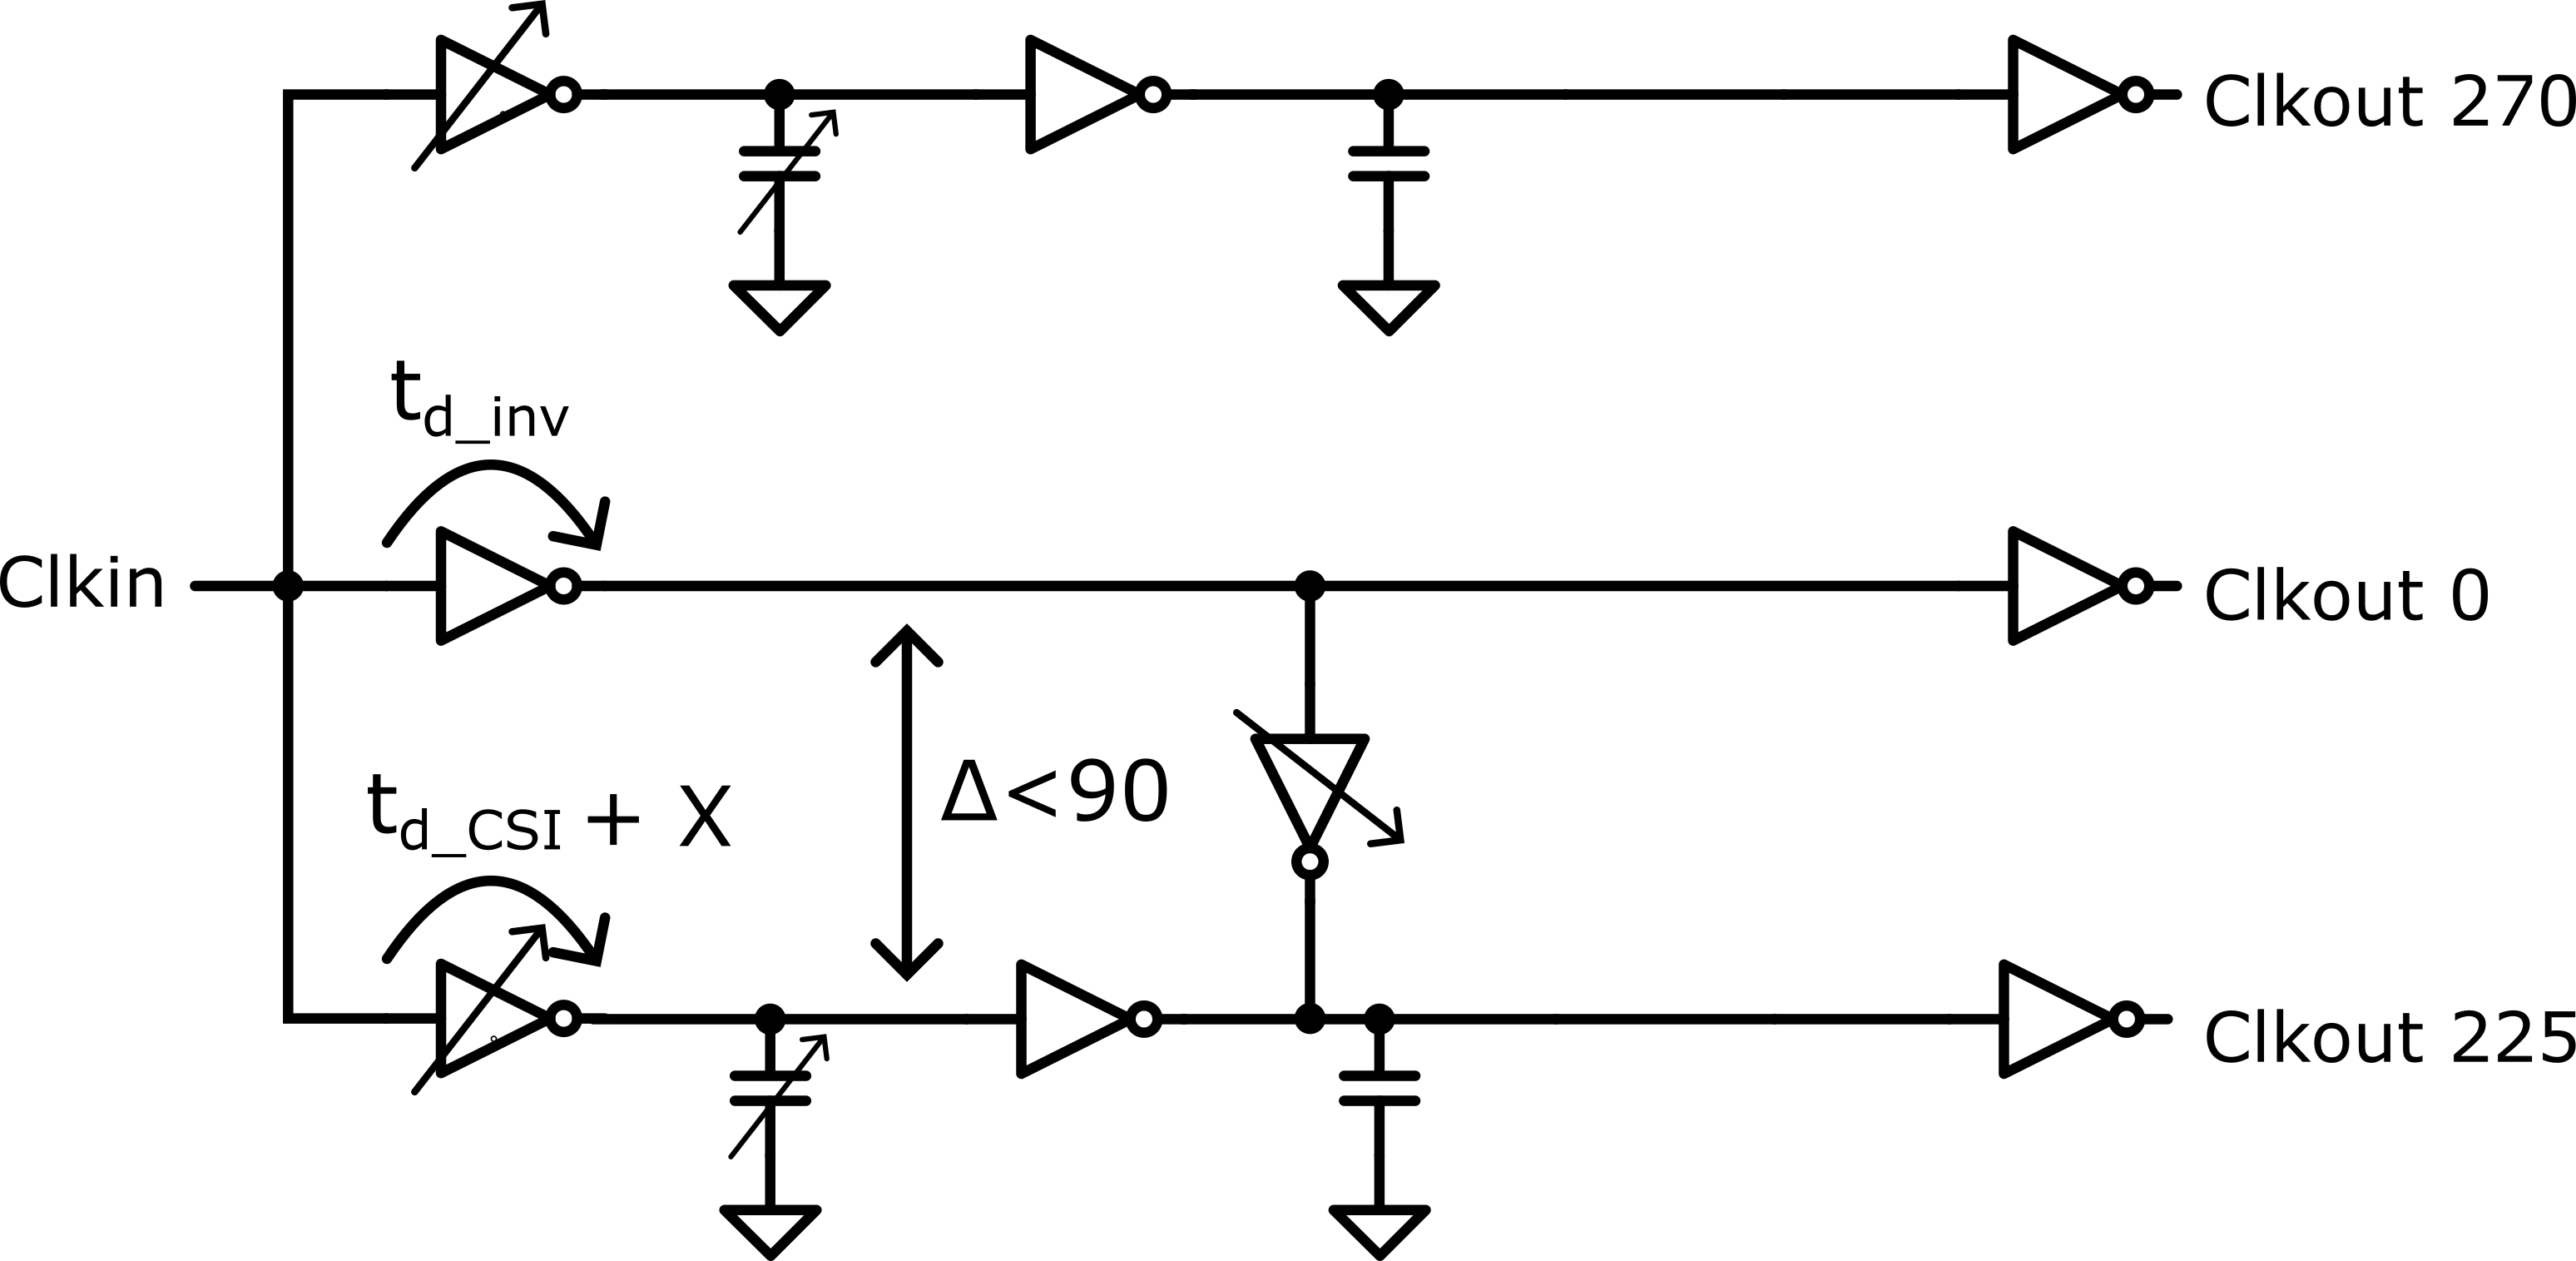
\includegraphics[width=0.8\linewidth]{figures/Schematics/ff_csi_3out.png}
  \caption{Feed-forward phase interpolator with internal node with phase $\approx$\ang{180} feeding into a second intermediate node with delay  $\approx$\ang{135}.}
  \label{fig:FF_half_1}
\end{figure}

Figure~\ref{fig:FF_half_veriloga_tuning} shows the VerilogA block tuning the feed-forward implementation. The capacitance coarse steps followed by fine-tuning the bias voltages of the current-starved inverter (CSI) are clearly indentifiable as phase shift steps in the output clock over time.

\begin{figure}[H]
  \centering
  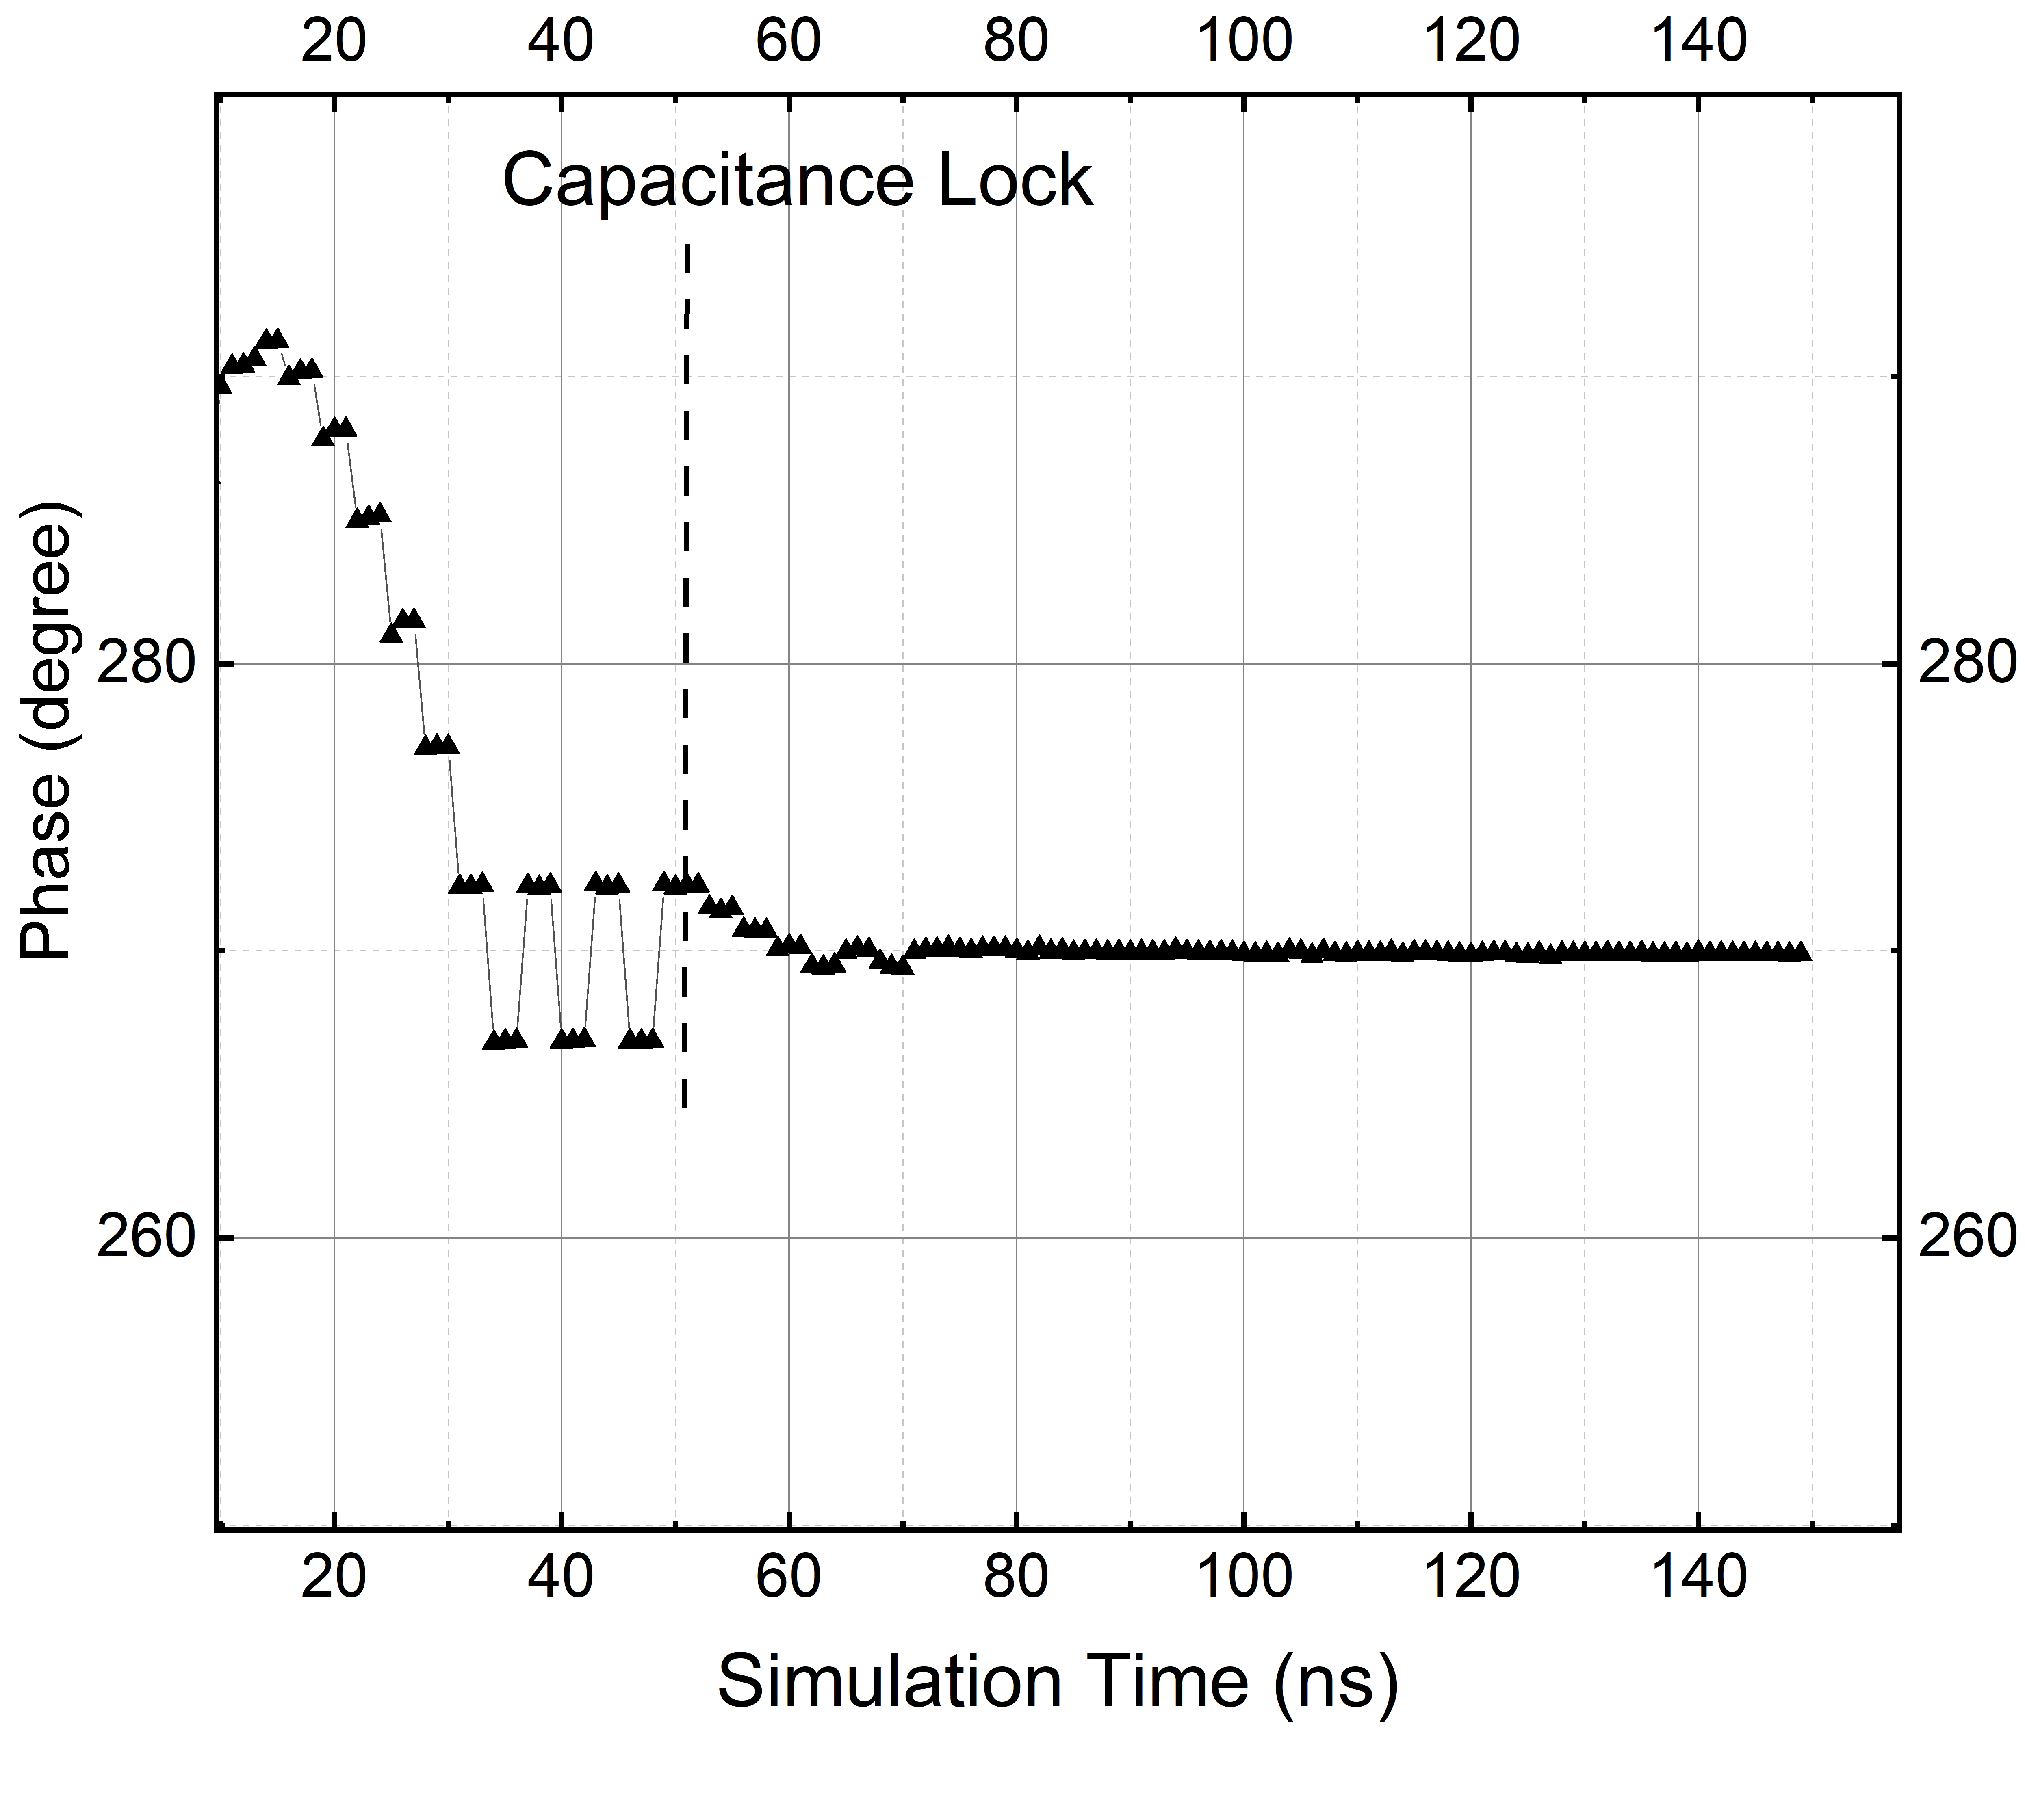
\includegraphics[width=0.8\linewidth]{figures/Results/FF_3out_CSI_dynamicTuning-225And270TuningCapAndVb.png}
  \caption{VerilogA tuning of the feed-forward phase interpolator. The coarse steps are followed by fine-tuning the bias voltages of the current-starved inverter (CSI).}
  \label{fig:FF_half_veriloga_tuning}
\end{figure}

\section{8-phase generation using feed-forwarding}\label{sec:8phase_FF}

Extending the three-output feed-forward architecture to an eight-output implementation introduced new challenges. Specifically, the initial strategy for generating the \ang{135} and \ang{315} phases proved ineffective. The feed-forward path from phase \ang{0} into the \ang{135}/\ang{315} branches, where the delay between internal nodes was still less than \ang{90}, resulted in the mixing of signals that were nearly \ang{135} or \ang{180} out of phase, rather than the intended \ang{45} or \ang{90}.

This issue was resolved by restructuring the mixing topology (Figure~\ref{fig:FF_8out}). Instead of feeding forward from phase \ang{0}, the design was modified to mix phases \ang{270} and \ang{90} into the paths for \ang{0} (\ang{360}) and \ang{180}, respectively. Additionally, the tunable feed-forward inverters proved unnecessary, complicating the design while having negligible impact on the mixing quality. Concurrently, the inverters driving the \ang{0} and \ang{180} phases were deliberately weakened. The engineered strength imbalance between the two driving inverters further enhances the mixing behavior since the \ang{270} signal already experiences significant delay from multiple buffering stages, arriving at the mixing inverter with weakened drive strength. This configuration is more accurately described as a "feed-backward" approach, as it involves signals from later phases accelerating the transitions of earlier ones, though it is still referred to as feed-forwarding for consistency with the original architecture.

\begin{figure}[H]
  \centering
  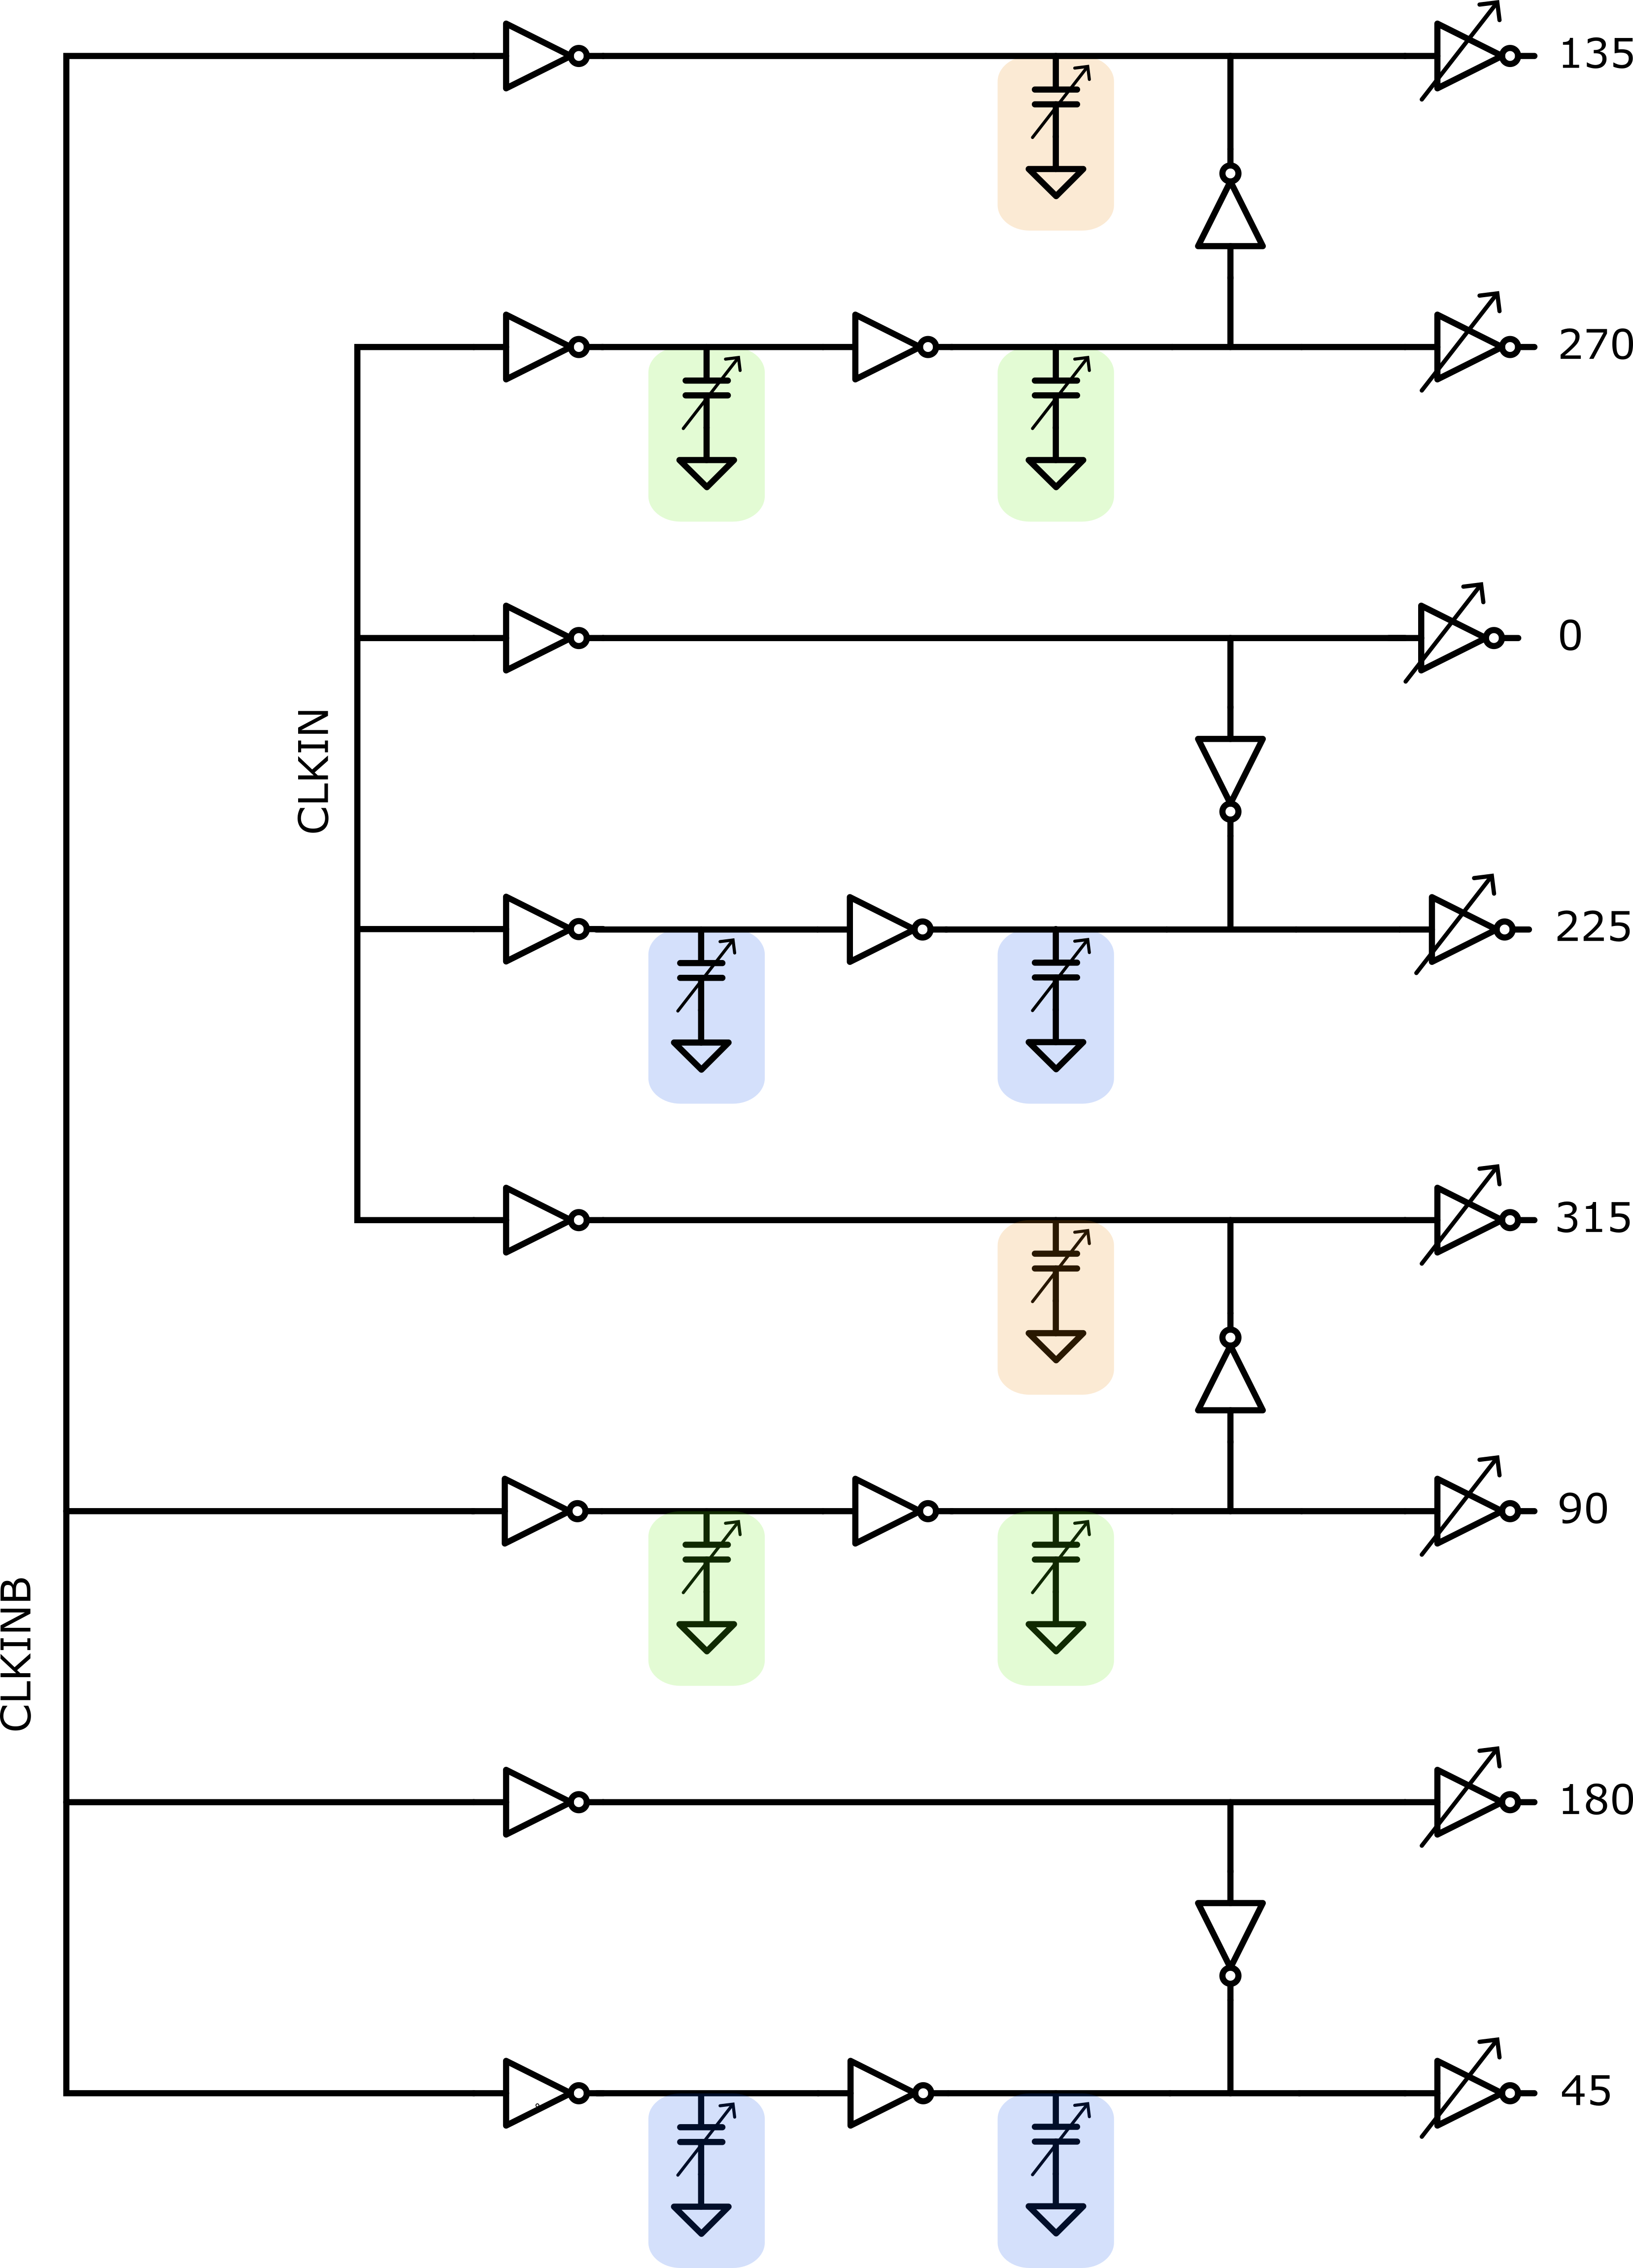
\includegraphics[width=0.8\linewidth]{figures/Schematics/ff_8out.png}
  \caption{Feed-forward phase interpolator with eight outputs. The \ang{135}/\ang{315} and \ang{45}/\ang{225} phases are generated by mixing the \ang{0}/\ang{180} and \ang{270}/\ang{90} phases into branches similar to those of \ang{0}/\ang{180} and \ang{270}/\ang{90} phases, respectively.}
  \label{fig:FF_8out}
\end{figure}

\section{3nm Porting}\label{sec:3nm_porting}

Following its successful implementation in 7nm, the 8-phase feed-forwarding architecture was ported to a 3nm technology node. This was necessary to meet the higher target frequency of 22.5GHz, which was unattainable with the 7nm design. The porting process involved adapting the design to the new technology's characteristics, including transistor sizing and capacitance values.

The ported design retained the core feed-forward architectural principles. However, adjustments were made to account for the different properties of the 3nm transistors, such as threshold voltages and drive strengths, and the tuning mechanisms were recalibrated. Jitter performance was verified using both transient and periodic noise (pnoise) simulations. After establishing a correlation between the two methods and adjusting simulation parameters, pnoise analysis was used exclusively for faster verification.

The initial 3nm design failed to meet jitter specifications, which necessitated doubling transistor sizes. While the capacitance and bias voltage tuning blocks successfully tuned the phases across Process, Voltage, and Temperature (PVT) variations, it was noted that the minimum capacitance of the MOS capacitor banks was higher than desired. This led to a reduction of most static capacitances in the circuit to compensate for this effect. The purpose of static capacitanes had been to provide a fixed delay shift in designs where the range of the tunable capacitors was sufficiently large, but consistently too low, meaning only the (e.g.) lower 70\% of the total available codes were being used. Higher frequencies, however, naturally required less total capacitance, and the static capacitances were not needed to achieve the required phase shifts. 

\section{Frequency range increase to 11GHz - 22.5GHz}\label{sec:freq_range}

The design was further adapted to operate across a wide frequency range from 11GHz to 22.5GHz. This required resizing the capacitor banks to ensure adequate phase shift control across the entire spectrum. This resizing led to an increase in the bank's total needed capacitance, which consequently increased the parasitic off capacitance as well.

The static capacitance values on most nodes were further reduced, in many cases to zero, making the capacitor banks the sole source of tunable capacitance, which was an unexpected yet positive design change. Importantly, a larger total capacitance also meant a larger step size, reducing the tuning resolution. However, the fine-tuning mechanism using current-starved inverters was able to compensate for this coarse resolution, although this required careful monitoring. In Figure~\ref{fig:FF_8out_CSI_dynamicTuning_PVT}, the VerilogA tuning of the \ang{90} degree phase is shown, demonstrating the ability to dynamically adjust the phases across different PVT corners and frequencies. For demonstrative purposes, some corners were chosen where the vb tuning was not sufficient to achieve the target phase, necessitating the recall of the coarse tuning block to adjust the capacitance code.

\begin{figure}[H]
  \centering
  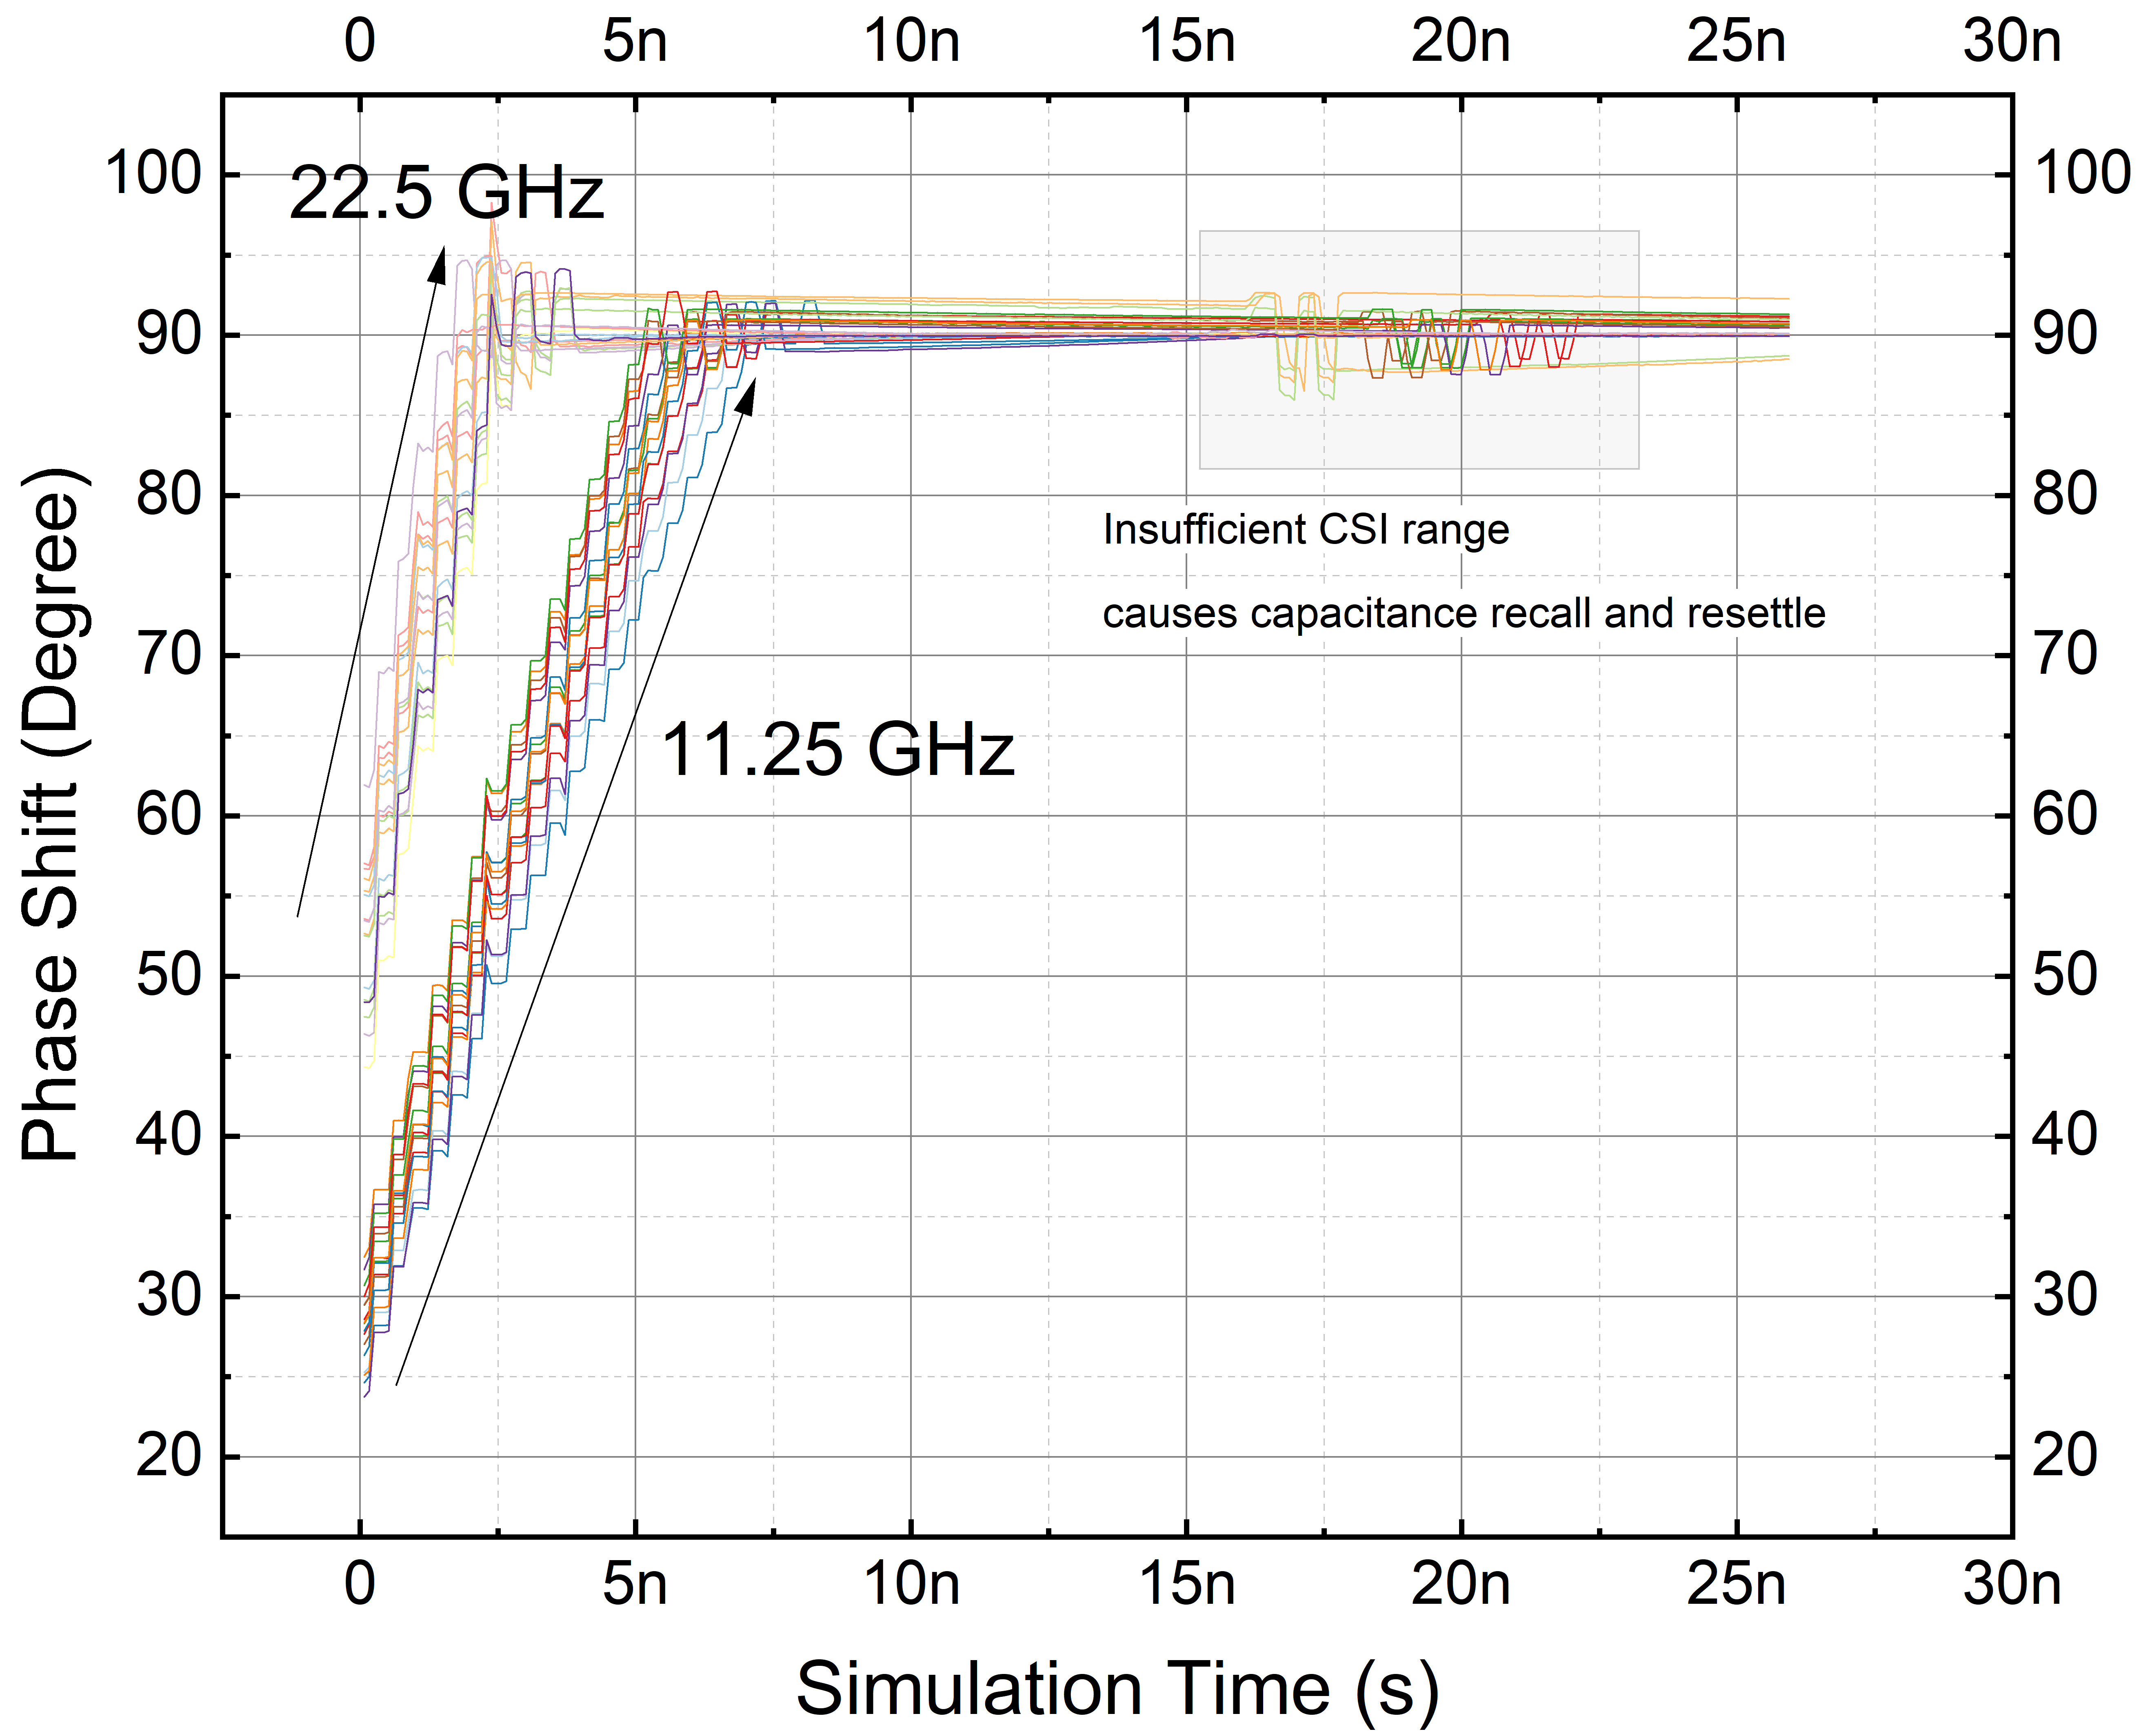
\includegraphics[width=0.8\linewidth]{figures/Results/FF_8out_3nm_idealswitches-Phase90_tuning_PVT_SomeN.png}
  \caption{VerilogA tuning of the 8-phase feed-forward architecture across different PVT corners. The coarse tuning block is recalled when the fine-tuning is insufficient to achieve the target phase.}
  \label{fig:FF_8out_CSI_dynamicTuning_PVT}
\end{figure}

\subsection{Capacitance bank behavior and duty-cycle distortions}

It was observed that at lower frequencies (e.g., 11GHz), the higher total capacitance required for tuning unexpectedly caused duty-cycle distortions. Investigation revealed that the capacitance of the MOS-based capacitor bank was highly dependent on the voltage of the node it was connected to. This voltage-dependent capacitance caused signals to have asymmetric rise and fall times, shifting the signal's crossing point away from half-supply and creating a perceived DCD (Figure~\ref{fig:FF_CapDCD}).

\begin{figure}[H]
  \centering
  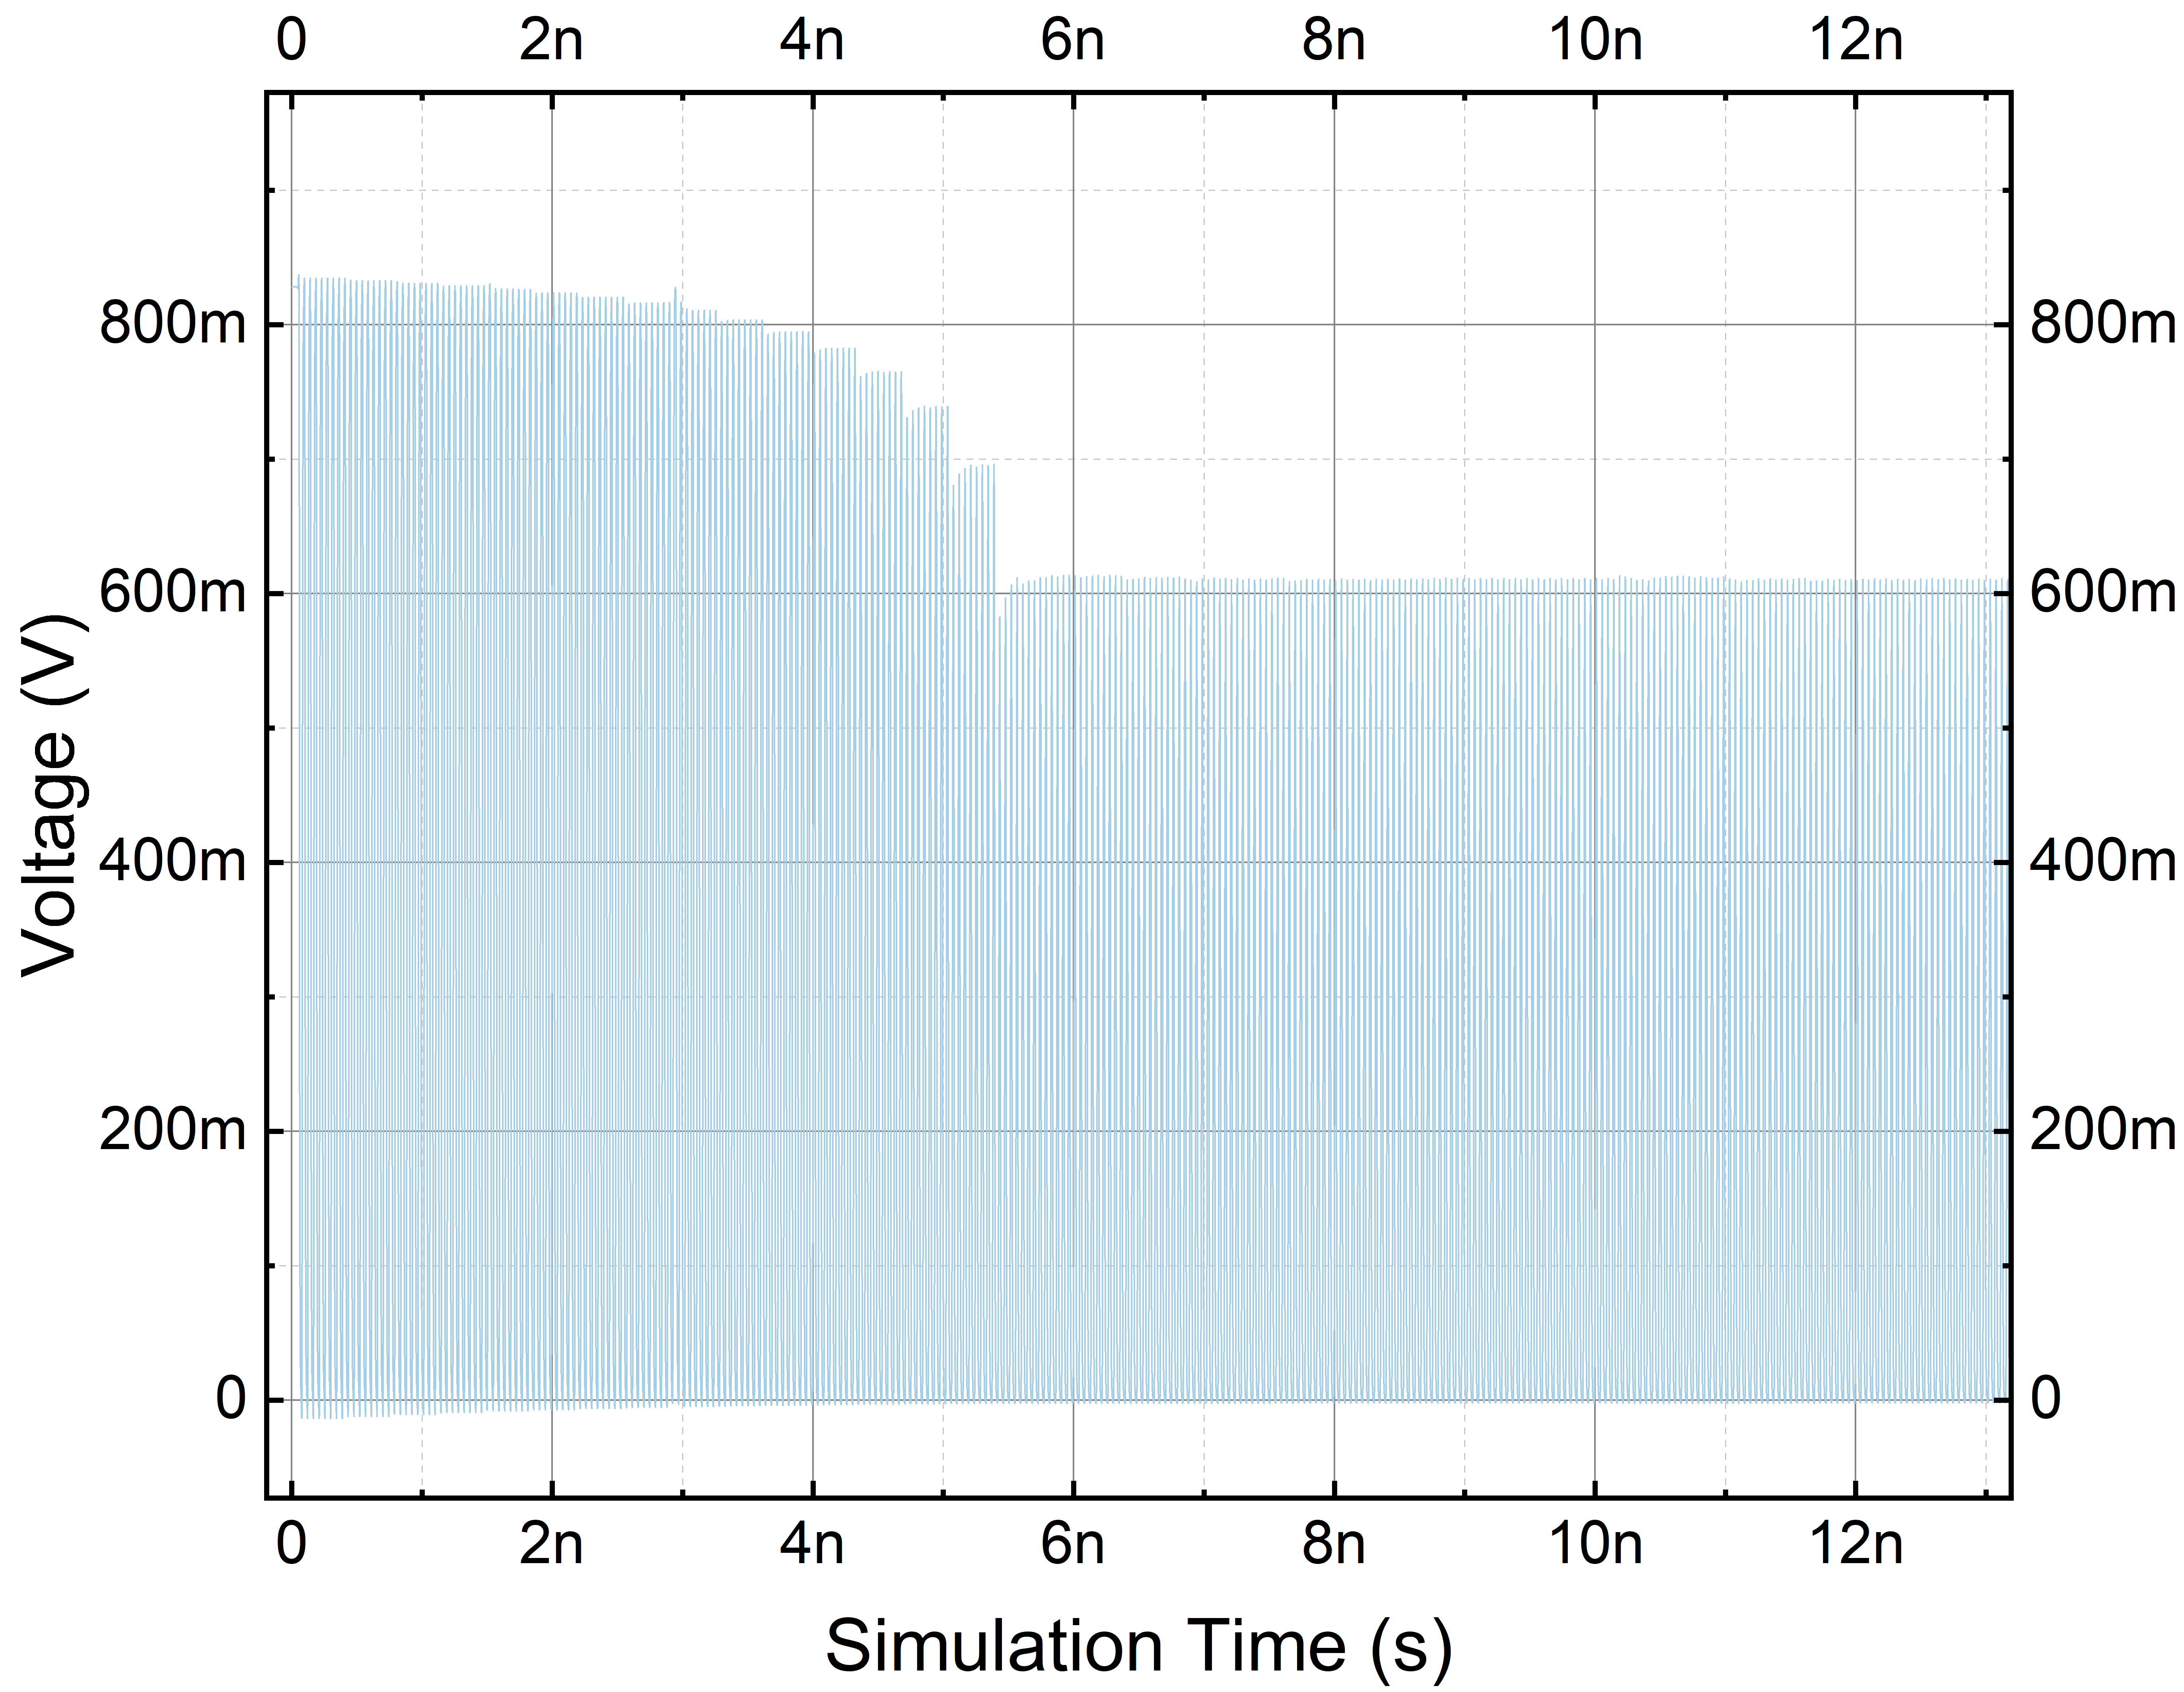
\includegraphics[width=0.8\linewidth]{figures/Results/FF_8out_PPNN-DCDWithCap.png}
  \caption{Duty-cycle distortion caused by the voltage-dependent capacitance of the MOS-based capacitor bank. The wave mid-point is shifted away from half-supply, leading to a perceived DCD.}
  \label{fig:FF_CapDCD}
\end{figure}

This issue was mitigated by splitting the capacitor bank into two separate branches: one composed of NMOS transistors connected to ground, and another of PMOS transistors connected to VDD. Since the capacitance of an NMOS device increases with gate voltage while that of a PMOS device decreases, this dual-branch structure provides a more constant total capacitance across the signal voltage swing.

Three different dual-branch capacitor bank implementations were explored:
\begin{itemize}
    \item \textbf{"2P2N" Capacitor Bank:} What will hereafter be referred to as the "2P2N" capacitor bank (Figure~\ref{fig:2P2N_cap}) consists of an upper branch composed of a PMOS capacitor connected to the tap through a PMOS transistor, and a lower branch composed of an NMOS capacitor connected to the tap through an NMOS transistor. 
    \item \textbf{Tgate Capacitor Bank:} The "Tgate" capacitor bank (Figure~\ref{fig:Tgate_cap}) consists of a PMOS capacitor connected to the tap through a Tgate switch, and an NMOS capacitor connected to the tap through a second Tgate switch.
    \item \textbf{"PNPN" Capacitor Bank:} What will henceforth be called "PNPN" capacitor bank (Figure~\ref{fig:PNPN_cap}) consists of a PMOS capacitor connected to the tap through an NMOS transistor, and an NMOS capacitor connected to the tap through a PMOS transistor. The rational for this design is that the NMOS switch will more easily pull the voltage at the PMOS capacitor tap down, while the PMOS switch will more easily pull the voltage at the NMOS capacitor tap up. Since the PMOS capacitance increases with decreasing gate voltage, and the NMOS capacitance increases with increasing gate voltage, this design was expected to provide a more stable capacitance across the voltage swing. The secondary objective was to reduce layout complexity when compared to the Tgate capacitor bank.
\end{itemize}
All capacitor banks were designed as a binary-weighted array of the unit cells shown in Figure~\ref{fig:2P2N_cap}, \ref{fig:Tgate_cap}, and \ref{fig:PNPN_cap}. Both the MOSCap and the switches scaled in the same proportions to keep RC delays constant across codes. 

\begin{figure}[H]
  \hfill
  \begin{subfigure}[b]{0.15\linewidth}
    \centering
    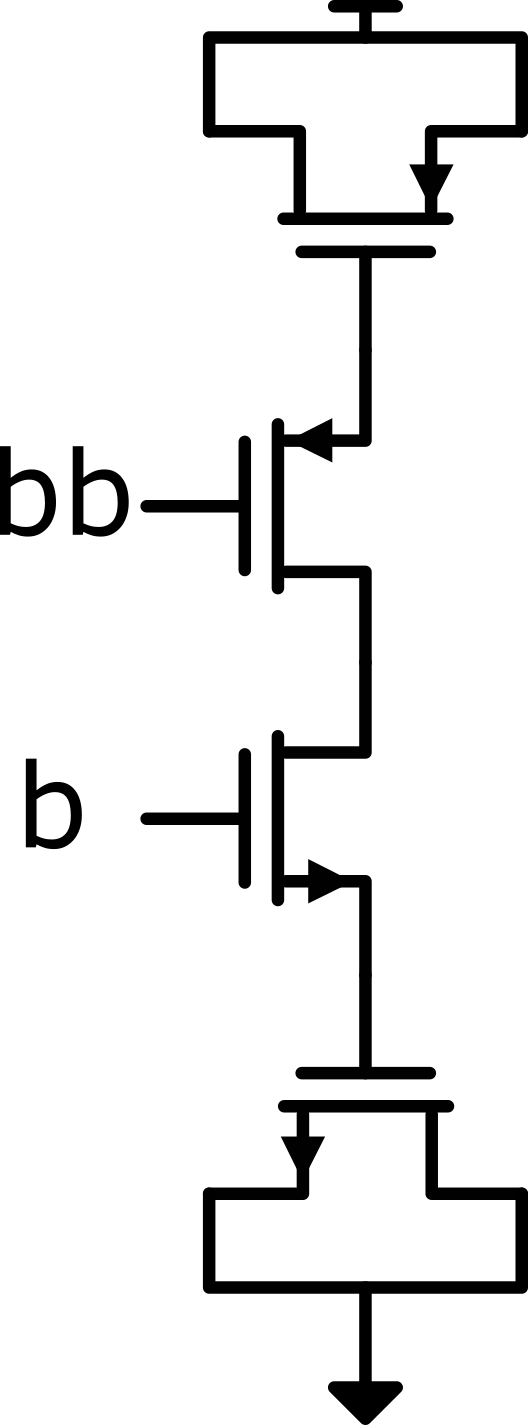
\includegraphics[width=\linewidth]{figures/Schematics/2P2N_cap.png}
    \caption{2P2N Capacitor Bank Unit Cell}
    \label{fig:2P2N_cap}
  \end{subfigure}
  \hfill
  \begin{subfigure}[b]{0.2\linewidth}
    \centering
    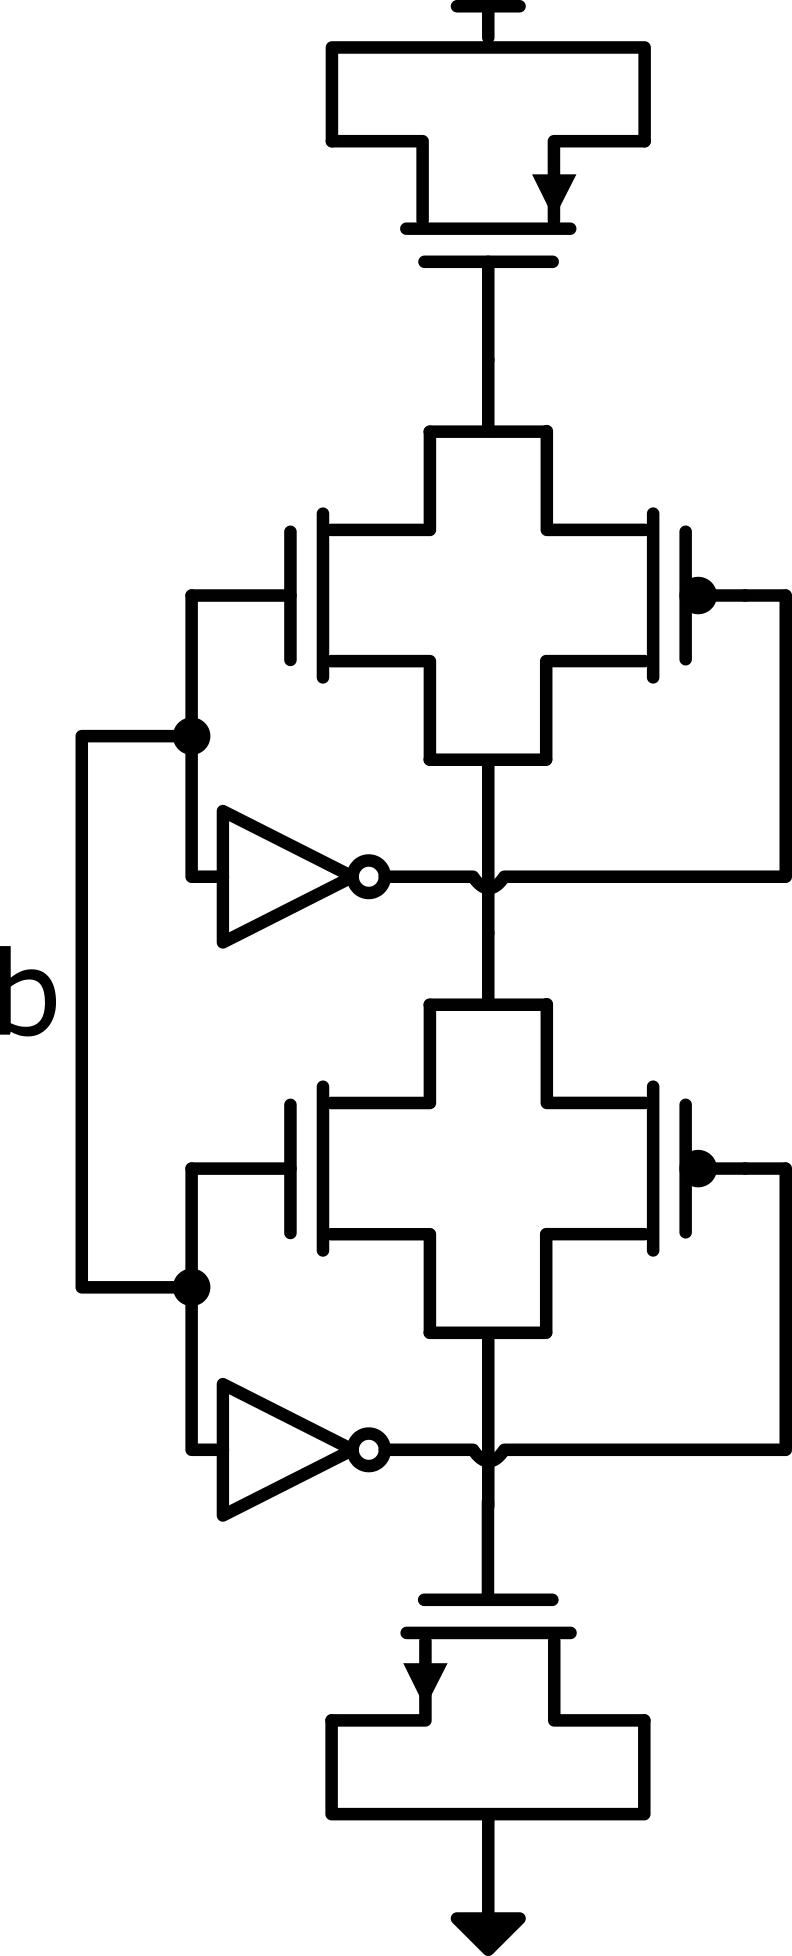
\includegraphics[width=\linewidth]{figures/Schematics/Tgate_cap.png}
    \caption{Tgate Capacitor Bank Unit Cell}
    \label{fig:Tgate_cap}
  \end{subfigure}
  \hfill
  \begin{subfigure}[b]{0.15\linewidth}
    \centering
    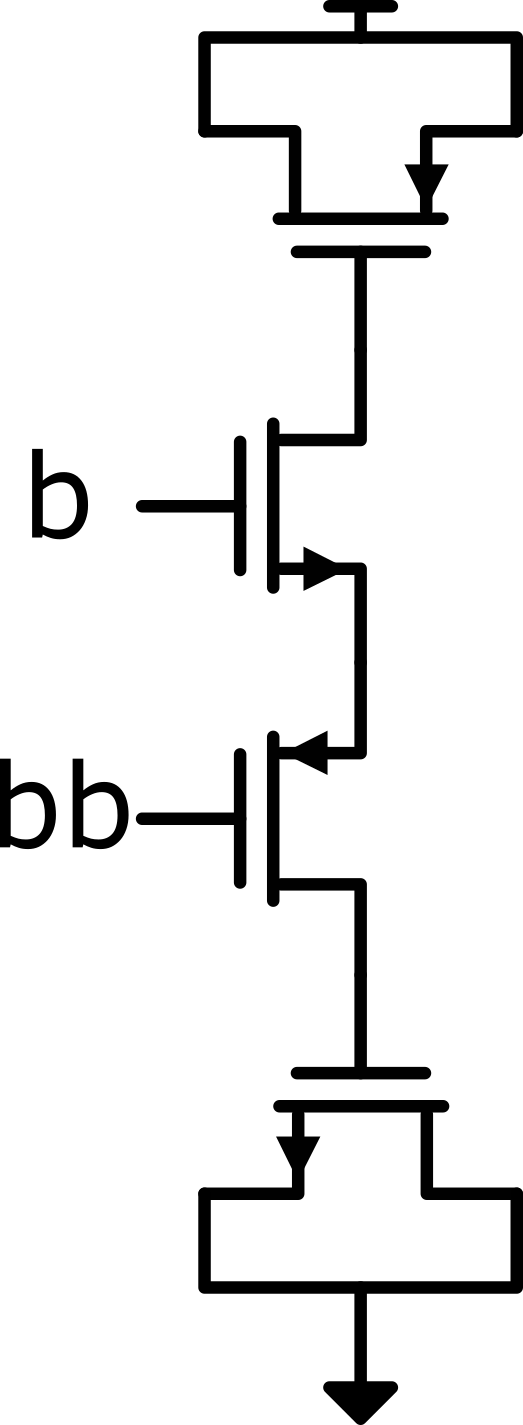
\includegraphics[width=\linewidth]{figures/Schematics/PNPN_cap.png}
    \caption{PNPN Capacitor Bank Unit Cell}
    \label{fig:PNPN_cap}
  \end{subfigure}
  \hfill\null
  \caption{Different capacitor bank implementations for the feed-forward phase interpolator.}
\end{figure}

A testbench was set-up to compare the performance of these three capacitor banks. The switch transistors and MOSCap sizings were set to the same values across all three banks for consistency. All three designs were controlled by an ideal 5-bit digital control. The testbench measured the step sizes of each bank across a range of frequencies, as well as the off capacitance at code 5b'00000. Beyond this, the capacitance values were also compared across tap voltages to assess the voltage dependency of the capacitance.

Capacitance values were extracted by running an ac simulation and subsequently extracting the imaginary part of the impedance at the tap node. This is expressed by the frequency-dependent equation:
\begin{equation}
  C_{\text{tap}}(F) = \frac{1}{2\pi f \textit{Im}(Z_{\text{tap}})}
\end{equation}

The 2P2N and PNPN capacitor banks were found to be similar in terms of step sizes across codes, while the Tgate consistently provided larger step sizes. Moreover, the Tgate capacitor bank exhibited the highest off capacitance (roughly double that of the 2P2N and PNPN banks), which was expected since even when the switch was off, there were a higher number of transistors connected to the tap node, leading to a larger parasitic capacitance.
Across tap voltages, the 2P2N and PNPN capacitor banks exhibited the less consistent capacitance values, with the 2P2N bank still showing a significant improvement in capacitance stability across tap voltages. The Tgate capacitor bank showed the most consistent capacitance values across tap voltages, with a very small variation.
Figures \ref{fig:cap_vs_codes} and \ref{fig:cap_vs_tap_voltage} verify these observations, showing the step sizes across codes and the capacitance values across tap voltages for each capacitor bank, sampled at 22.5~GHz.

\begin{figure}[H]
  \begin{subfigure}[t]{0.45\linewidth}
    \centering
    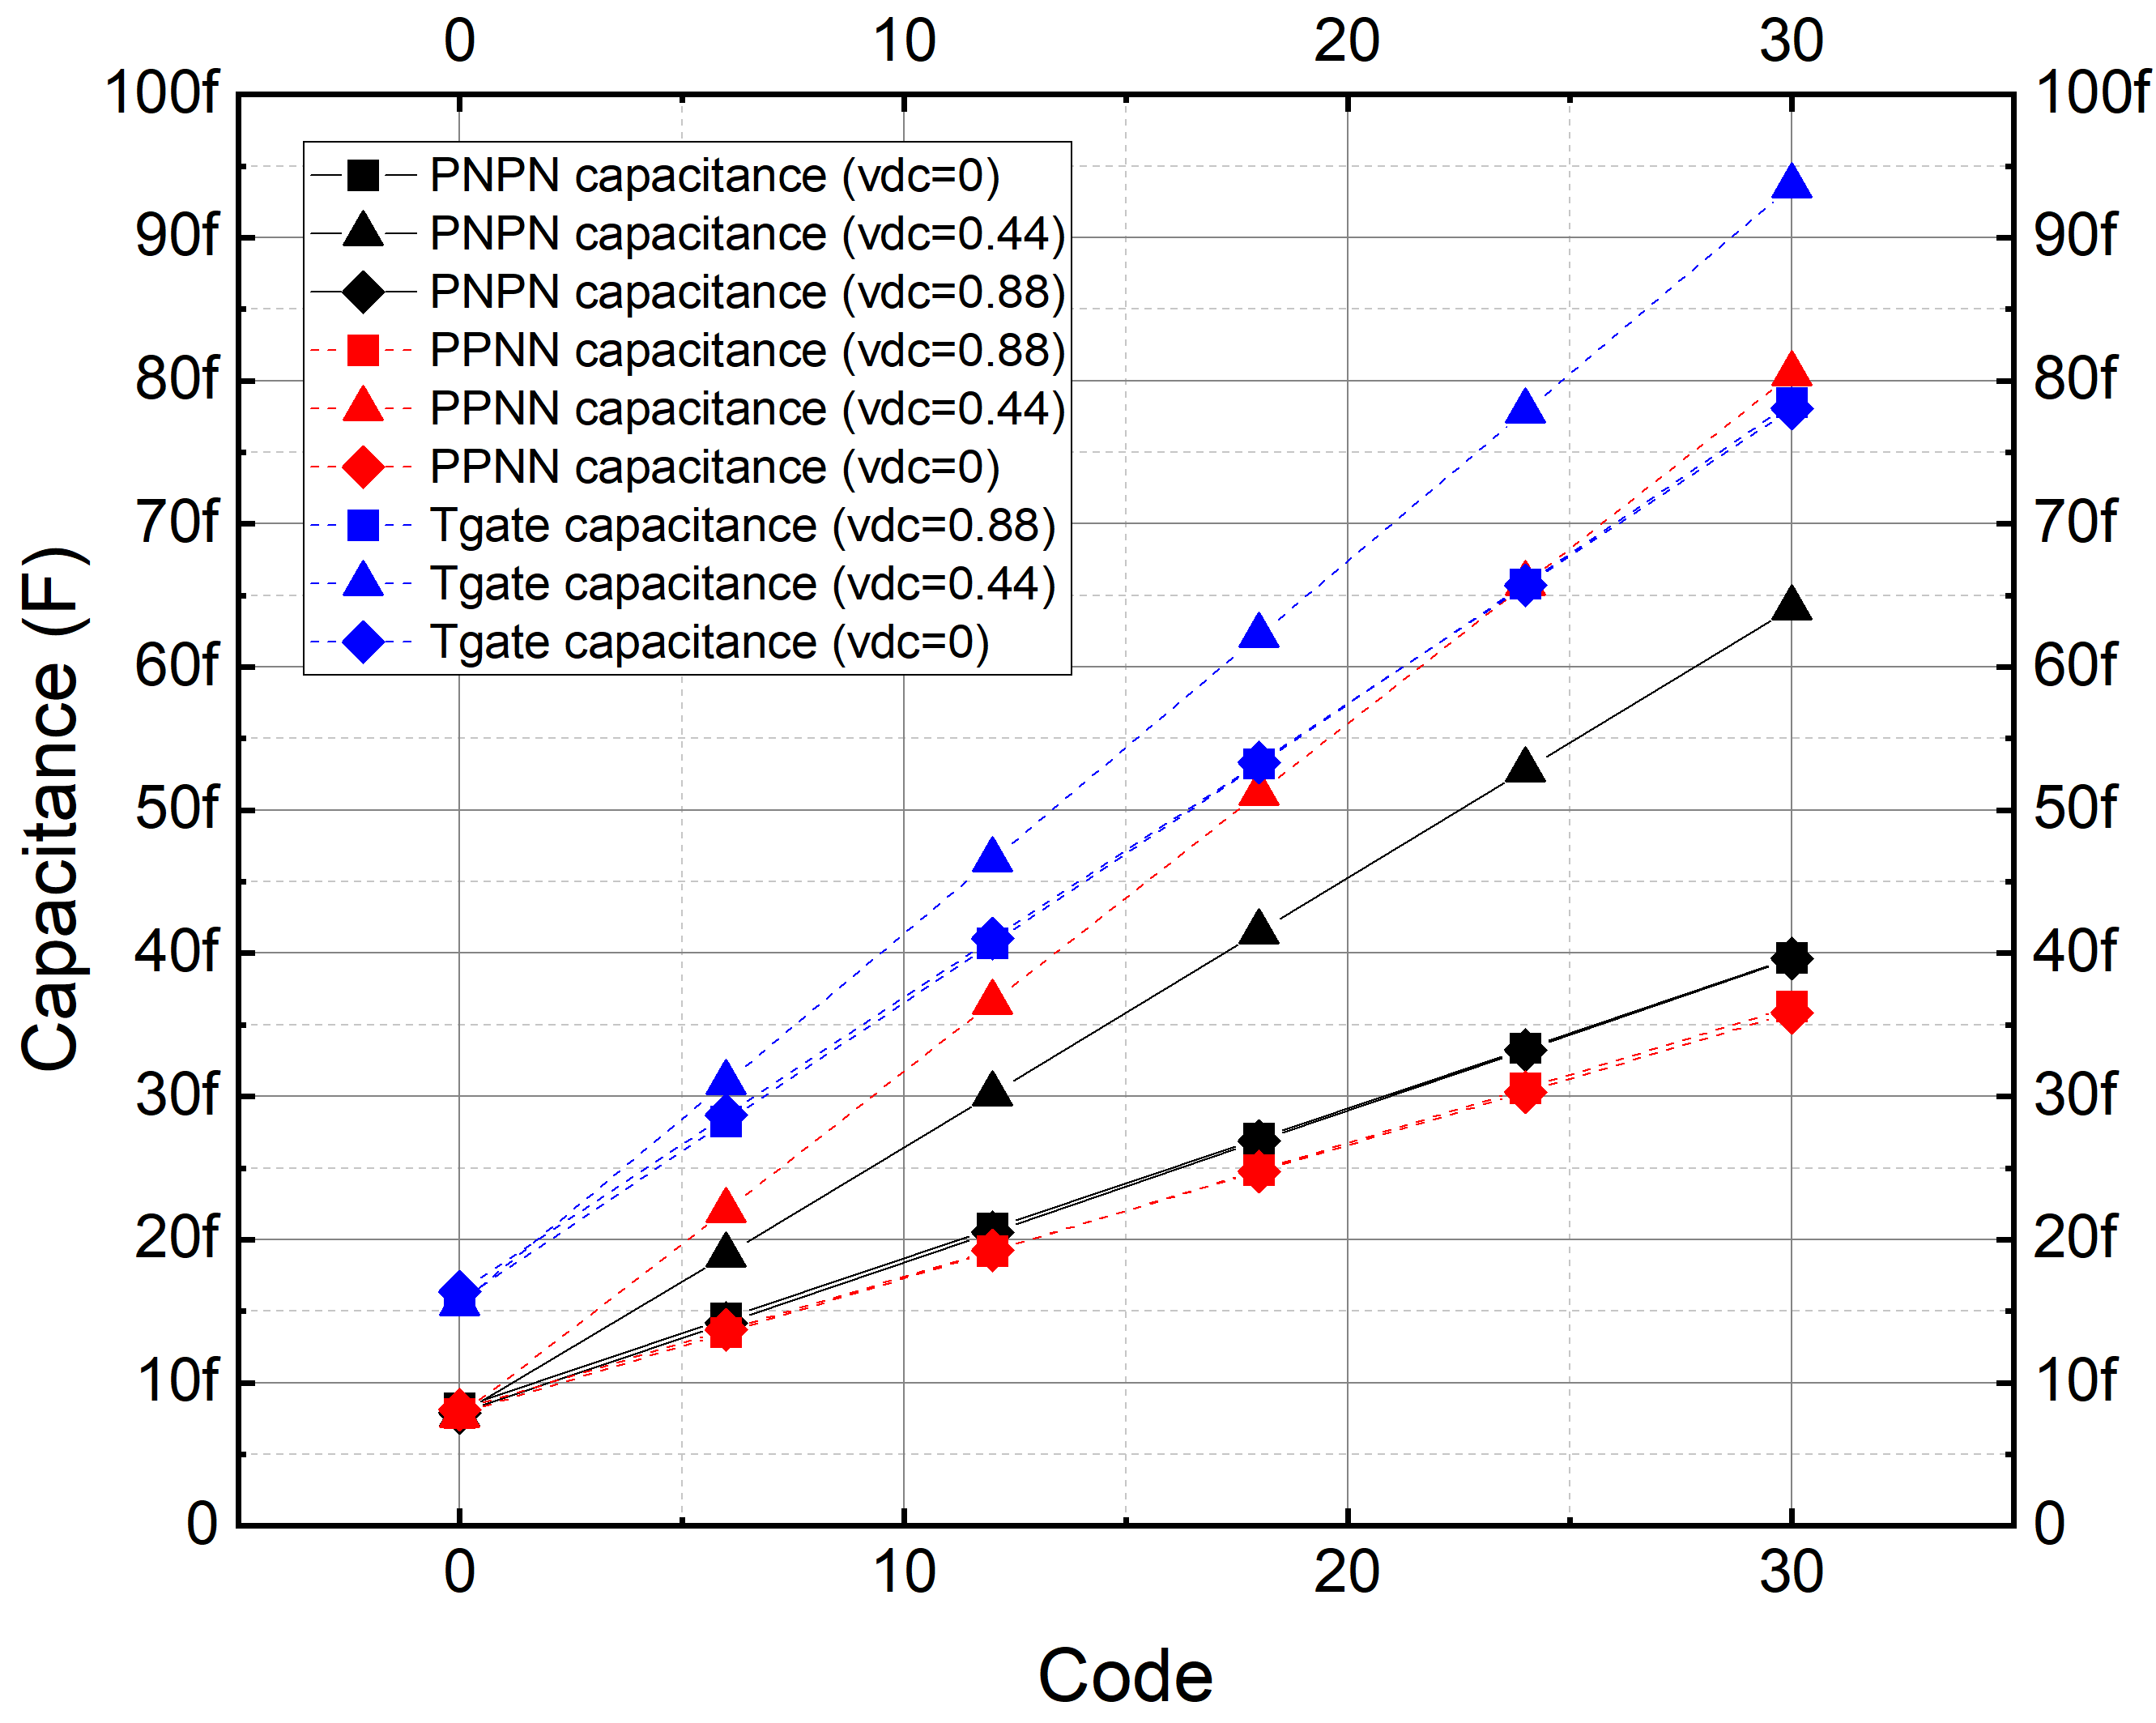
\includegraphics[width=\linewidth]{figures/Results/Cap_tests-CapVsCode.png}
    \caption{Capacitance step sizes across codes for the three capacitor bank implementations. The Tgate capacitor bank exhibits larger step sizes compared to the 2P2N and PNPN banks.}
    \label{fig:cap_vs_codes}
  \end{subfigure}
  \hfill
  \begin{subfigure}[t]{0.45\linewidth}
    \centering
    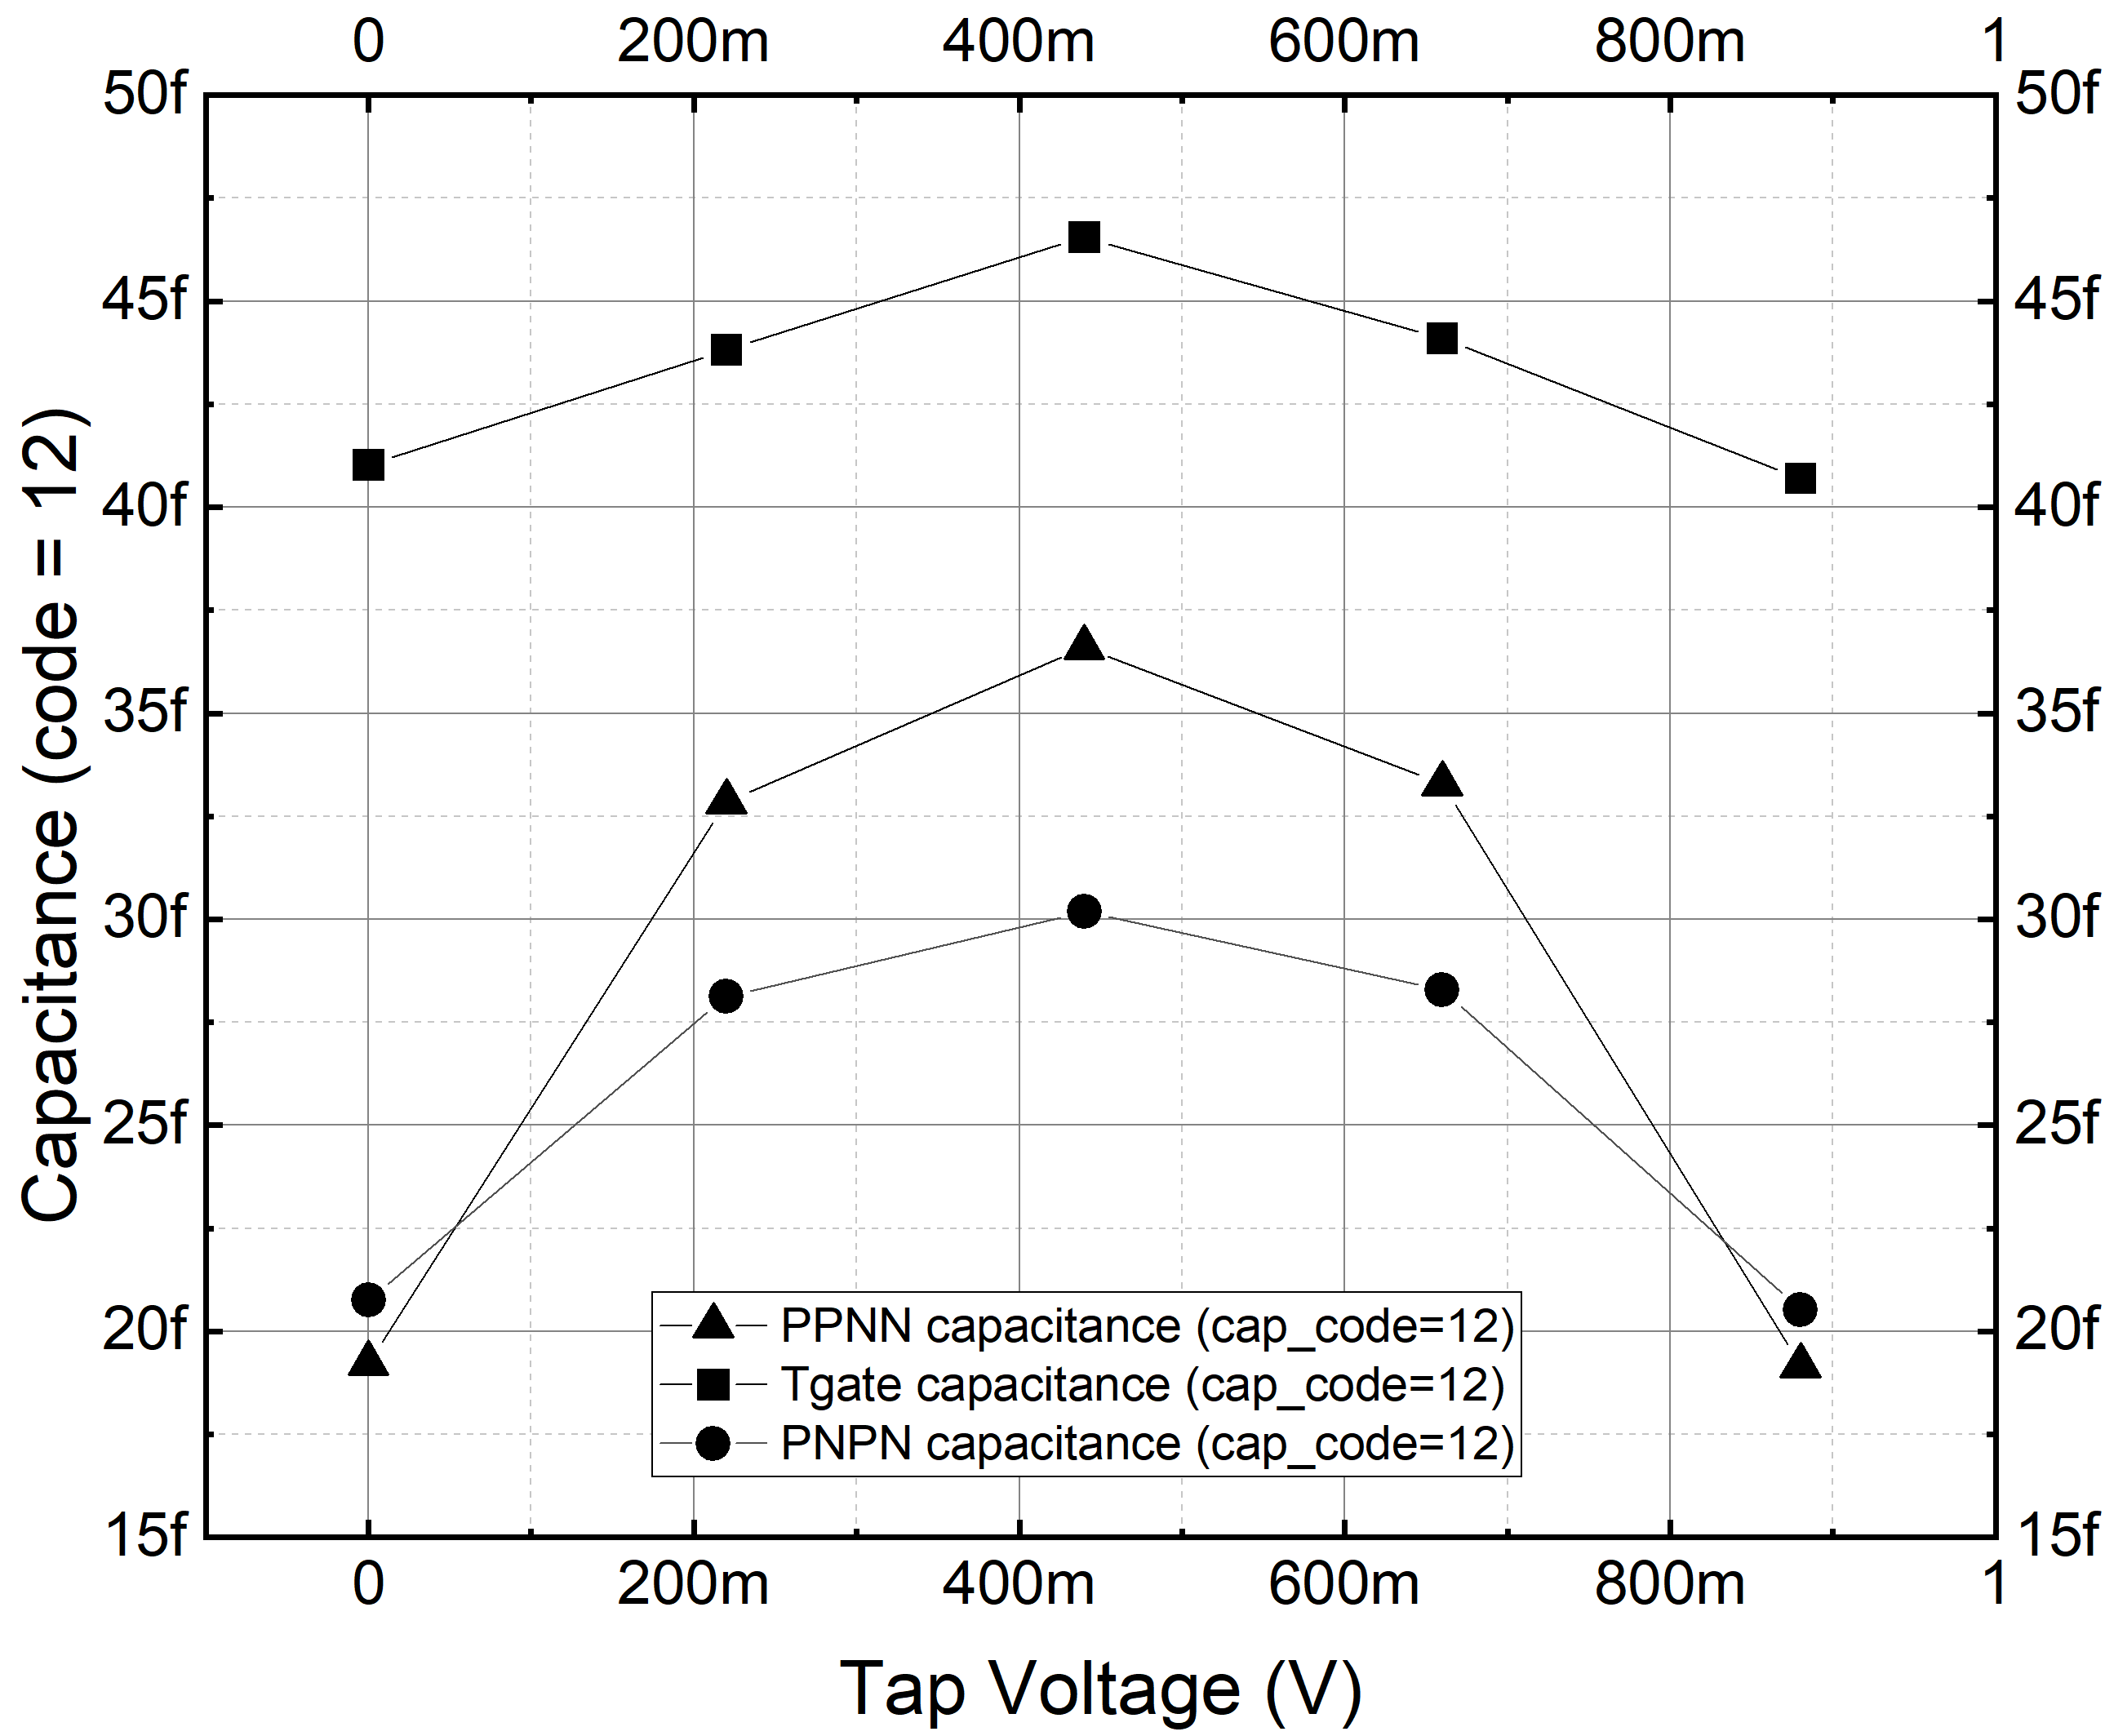
\includegraphics[width=\linewidth]{figures/Results/Cap_tests-CapVsVoltage.png}
    \caption{Capacitance values across tap voltages for the three capacitor bank implementations. The Tgate capacitor bank exhibits more consistent capacitance values compared to the 2P2N and PNPN banks.}
    \label{fig:cap_vs_tap_voltage}
  \end{subfigure}
\end{figure}

\subsection{Parasitic Back-Annotation Strategy}

To model post-layout behaviour we first back-annotated parasitic capacitances extracted with \textsc{ParagonX Pro}.%
The extracted values were inserted as ideal lumped capacitors between every relevant node pair (\(V_\text{IN}\), \(V_\text{OUT}\), \(V_\text{DD}\), \(V_\text{SS}\)) as drawn in Figure~\ref{fig:back_annotation}.

\begin{figure}
  \centering
  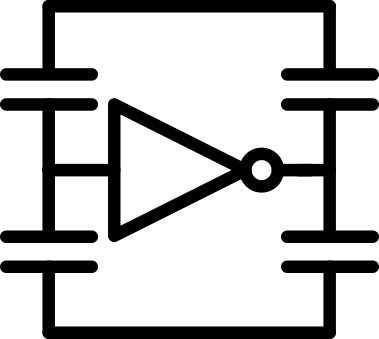
\includegraphics[width=0.2\linewidth]{figures/Schematics/BackAnnotation.png}
  \caption{Parasitic capacitances extracted with \textsc{ParagonX Pro} inserted as ideal lumped capacitors between every relevant node pair.}
  \label{fig:back_annotation}
\end{figure}

This initial experiment was performed on a simple buffer layout rather than the full 22.5 G–5 G multi-phase generator.
As a result, the reported parasitic caps were overly large and the back-annotated schematic failed at the target frequency: several clock phases collapsed or showed severe duty-cycle distortion across PVT corners.
Even with careful sizing of the MOS capacitors and switches, the parasitic load remained too high.
A second simulation was therefore carried out on a compact testbench.  
We compared (i) the transient response of this post-layout netlist with (ii) a schematic in which the extracted caps were multiplied by a global scaling factor.  
Good agreement appeared even when the scale factor was far below unity.  
Inspection of the DC operating point clarified the reason: the TSMC transistor wrapper models already include femtofarad-level capacitances beyond intrinsic and overlap capacitances that dominate most layout-dependent contributions at low metal levels.

Hence the wrapper-based schematic already mimics the bulk of the real parasitic capacitance.  
A fully accurate absolute back-annotation would require a specialised, fully optimised layout well beyond the exploratory buffer used here yet side-by-side comparisons show that the schematic plus wrapper reproduces post-layout behaviour closely enough for the current stage of the project.
It was thus decided that back annotation was not to be introduced at this stage, with an expected future revision to include a more accurate back-annotation of the parasitics, once the design is more mature and the layout is available.

\section{Redesign in favor of pure delay implementation}\label{sec:second_redesign}

Although the feed-forward implementation successfully generated the eight clock phases, it exhibited instability in phases \ang{135} and \ang{315} under certain process corners. This instability occurred when the delay requirements of different branches came into conflict. For example, in a fast-fast (FF) corner, the \ang{90}/\ang{270} paths might require increased capacitance to add delay, while the \ang{135}/\ang{315} paths might require reduced capacitance. Since \ang{90} feeds into \ang{135}, the two branches are coupled, and the tuning of one phase directly affects the other, meaning both branches were "fighting" to achieve their respective delays. Figure~\ref{fig:FF_8out_225vs135} illustrates this issue, where the \ang{135} is overcorrected as a consequence of the \ang{270} phase being too fast, leading to the former needing to decrease codes to achieve the desired phase shift.

\begin{figure}[H]
  \centering
  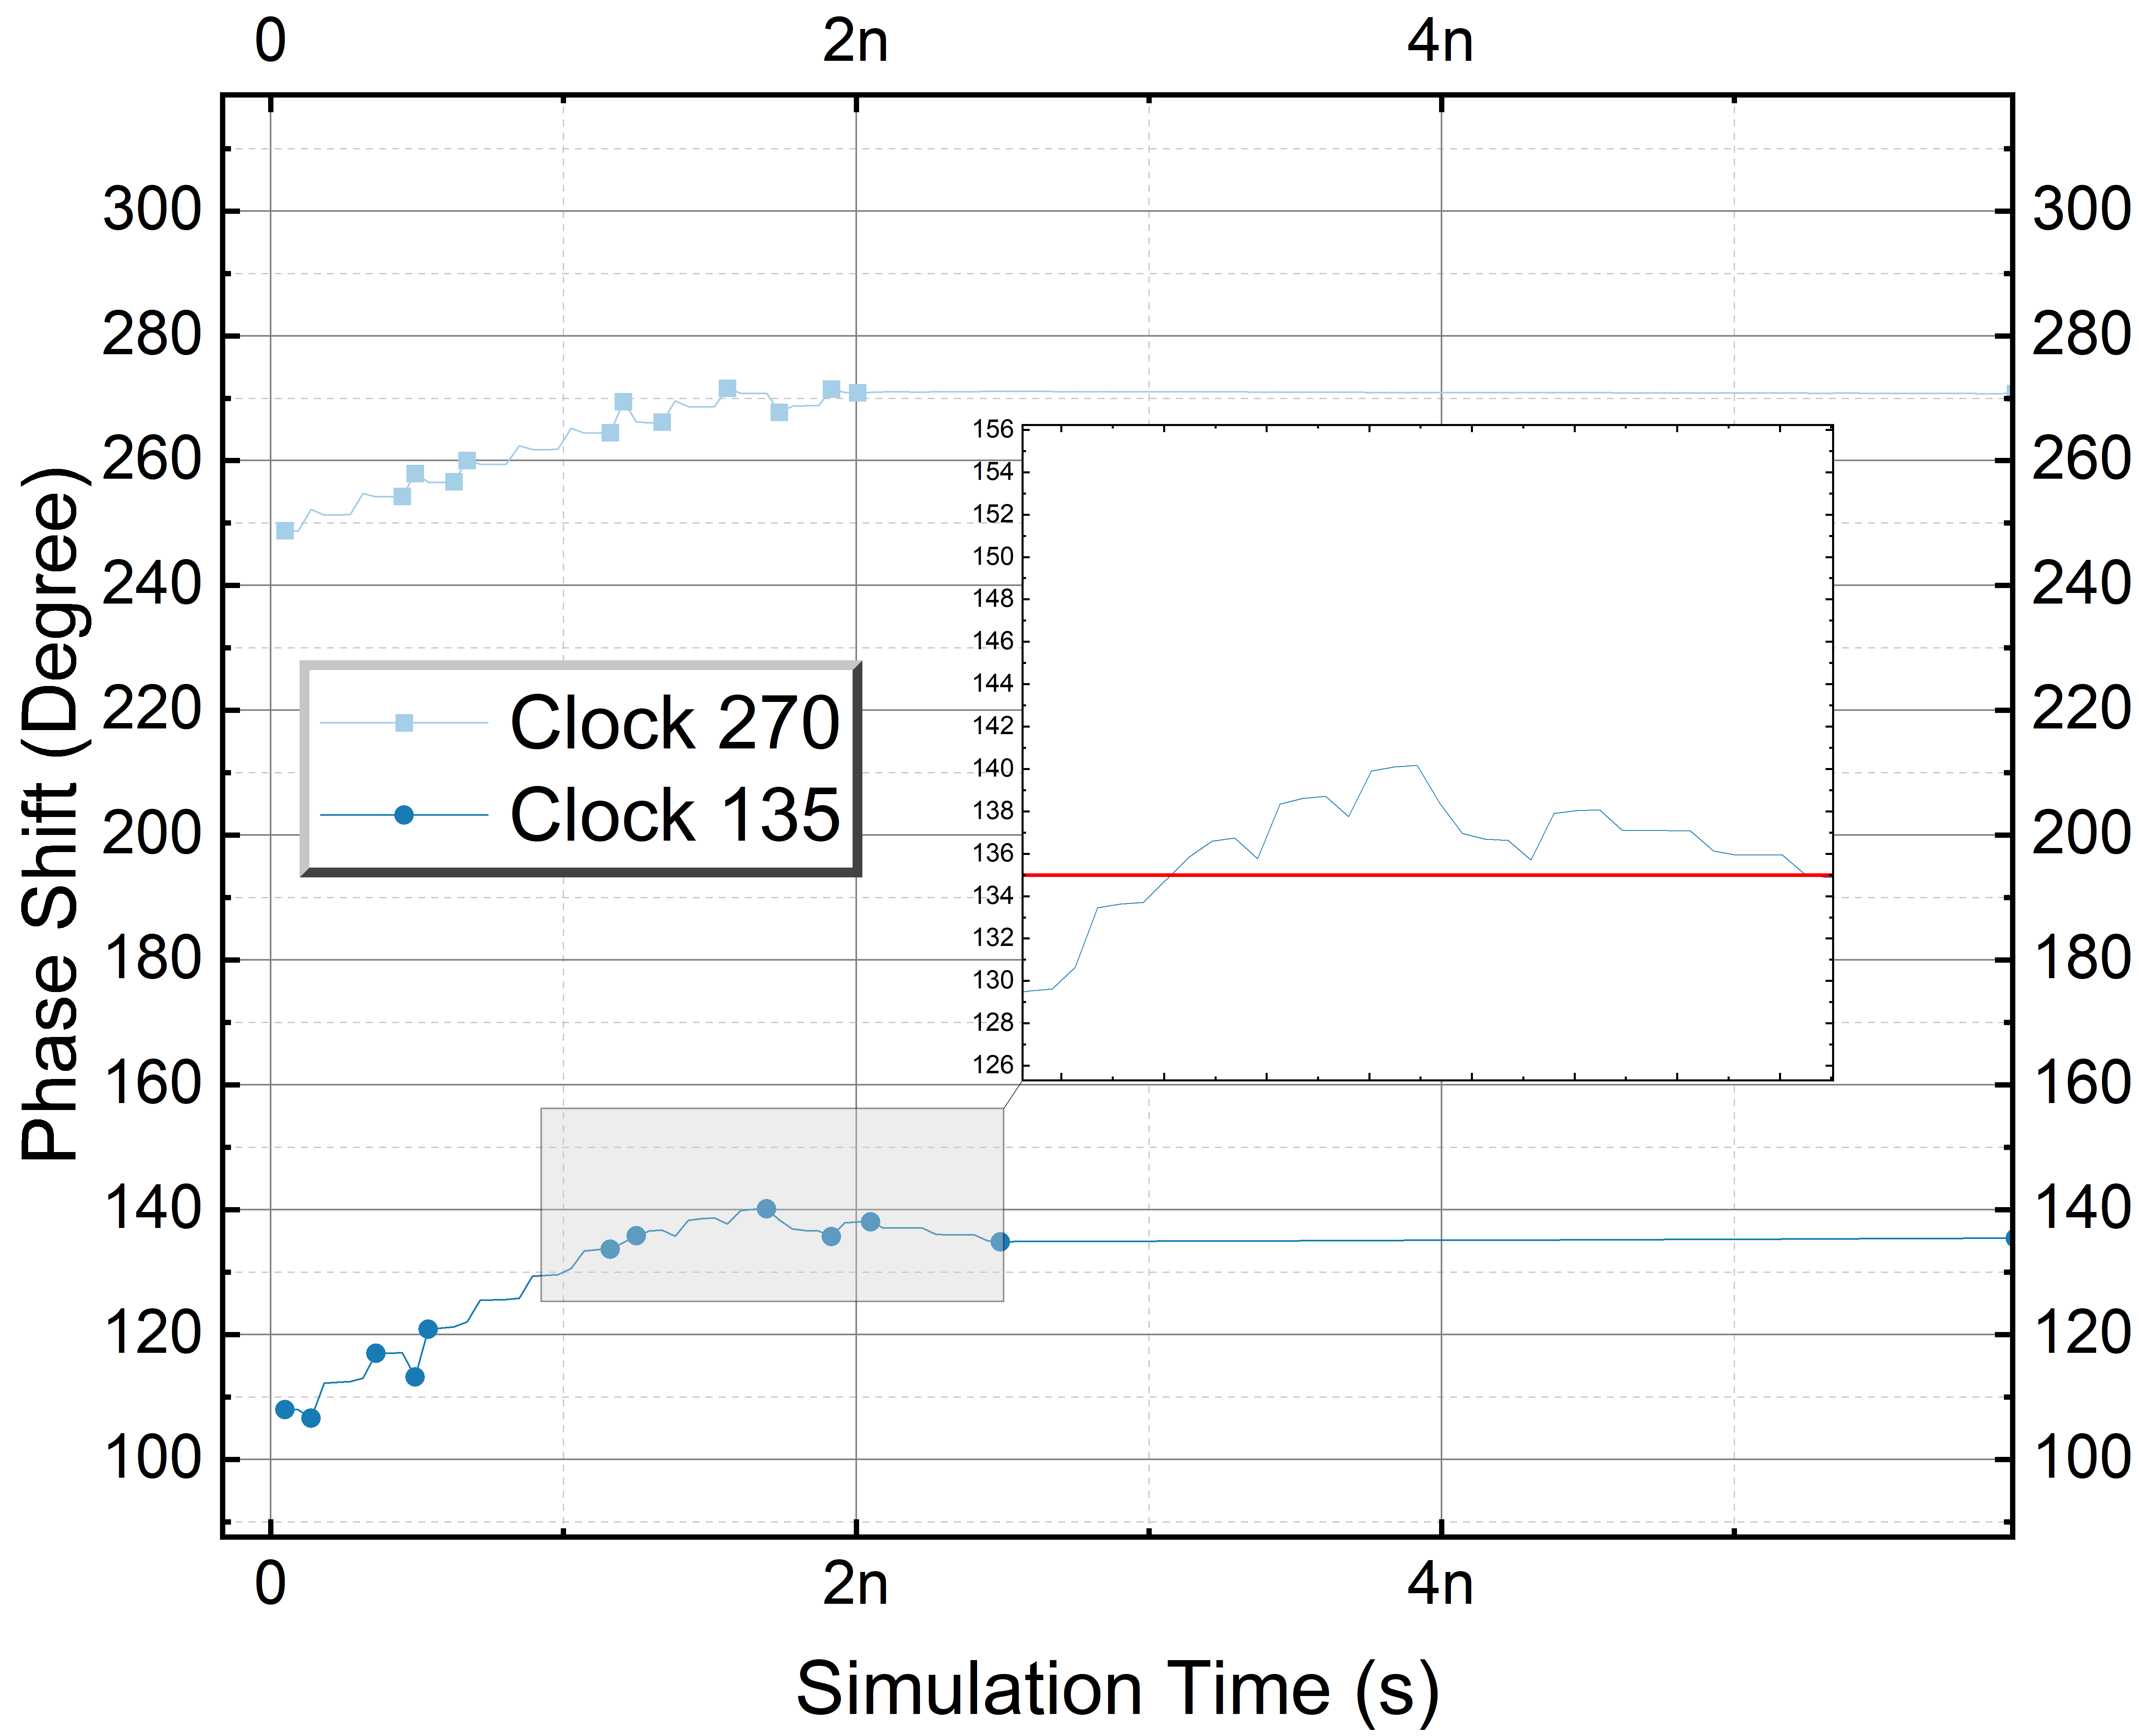
\includegraphics[width=0.8\linewidth]{figures/Results/FF_8out_PNPN-FightExample.png}
  \caption{Conflict between the \ang{270} and \ang{135} phases in the feed-forward implementation. The \ang{135} phase is overcorrected due to the \ang{270} phase being too fast, leading to a decrease in codes to achieve the desired phase shift.}
  \label{fig:FF_8out_225vs135}
\end{figure}

To address this fundamental issue, a second major redesign was undertaken, abandoning the feed-forward approach in favor of a pure delay implementation (Figure~\ref{fig:pure_delay}). This new architecture simplified the phase generation process by returning to a more traditional delay line structure, providing more consistent and, crucially, independent phase shifts for all eight outputs.

The new design retains eight independent delay paths but eliminates the feed-forward/backward mixing mechanism. Instead, it relies solely on a series of programmable delay elements within each path. This ensures that the tuning of one phase does not interfere with any other, resolving the stability issues observed with phases \ang{135} and \ang{315}.

\begin{figure}[H]
  \centering
  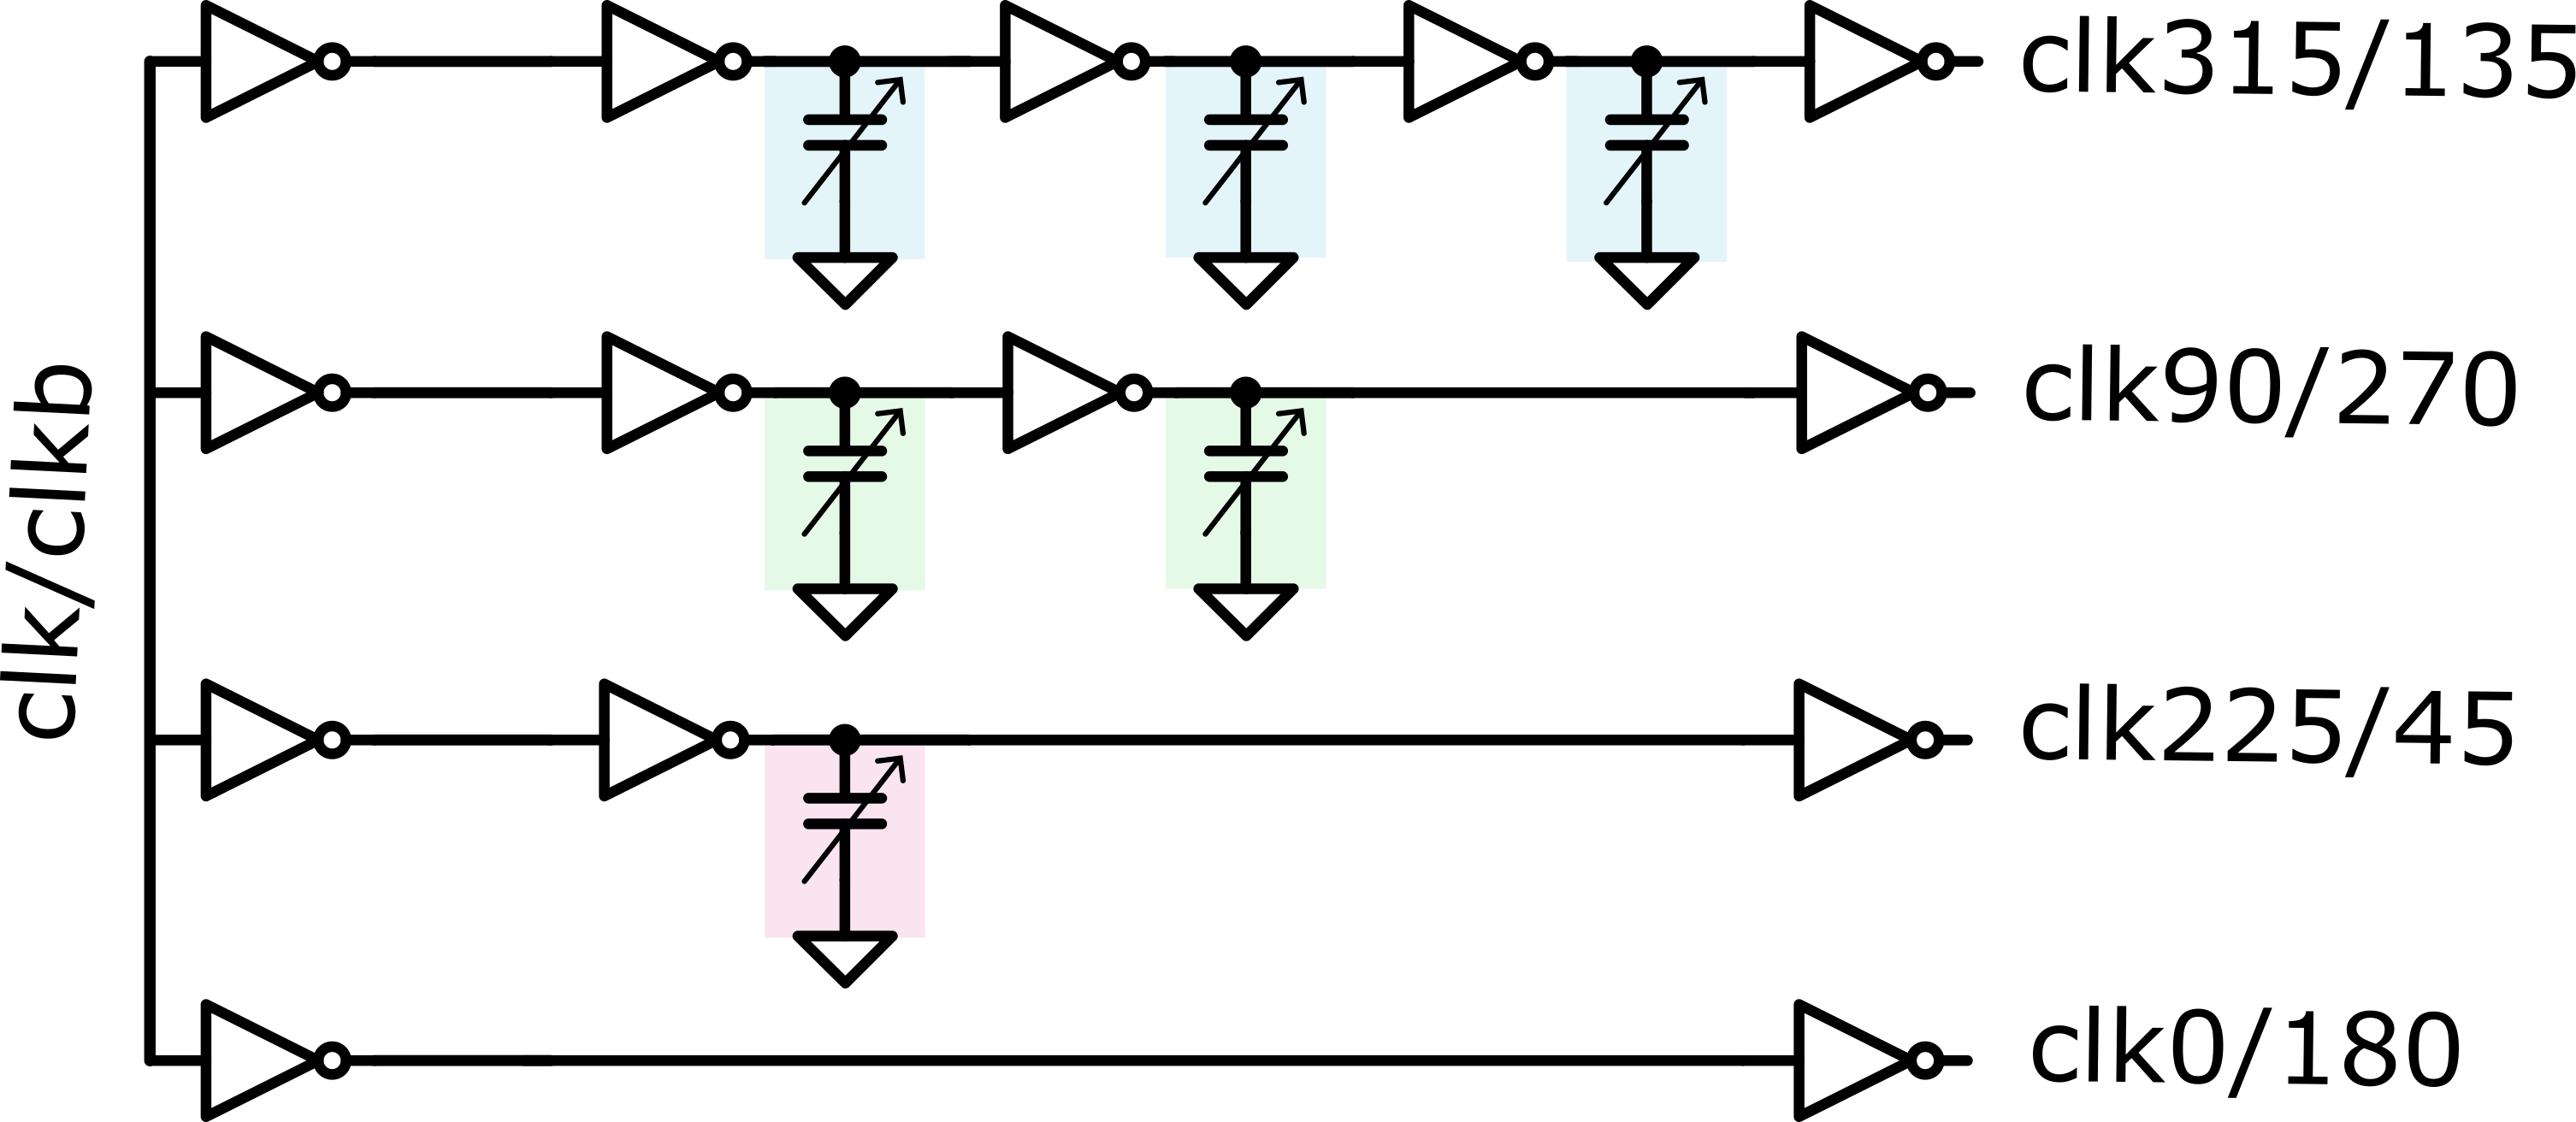
\includegraphics[width=0.8\linewidth]{figures/Schematics/pure_delay.png}
  \caption{Pure delay DLL architecture. Each of the eight phases is generated by a dedicated delay path, ensuring independent phase shifts and resolving stability issues observed in the feed-forward implementation.}
  \label{fig:pure_delay}
\end{figure}


Initially, a pure delay-line architecture had been discounted due to concerns about higher power consumption and potentially worse jitter performance compared to the feed-forward design. While the power consumption was indeed slightly higher, it was found that with careful design, the pure delay implementation could achieve comparable jitter performance.

A key observation was that spreading the required delay over a larger number of stages, each with a smaller capacitive load, led to lower jitter. This was attributed to two factors: 1) the improved slew rate of the less-loaded inverters, and 2) the increase of the low-pass cutoff frequency of each inverter stage, which improved the signal-to-noise ratio. As a result, every stage adds a delay of roughly \ang{45}, which results in phases \ang{315}/\ang{135} having a total of 5 cascaded inverters and phases \ang{90}/\ang{270}, \ang{225}/\ang{45} and \ang{0}/\ang{180} having 4, 3 and 2 cascaded inverters, respectively.
Another characteristic of this implementation is the different step sizes across the different phases, which is a consequence of the different number of capacitance banks in each path. The \ang{45} and \ang{225} phases have the smallest step sizes, while the \ang{315} and \ang{135} phases have the largest step sizes, as they have the most capacitance banks in their paths. This means that the \ang{315} and \ang{135} phases are likely to be the bottlenecks in terms of tuning resolution and jitter, owing in part to the high number of inverter stages.

The pure delay line was verified to operate correctly across the 11GHz to 22.5GHz frequency range, demonstrating improved phase stability and comparable jitter at the cost of moderately increased power consumption.

\section{Low-, Medium- and High-Speed Phase-Delay Element Final Implementation}\label{sec:mixF_design}

With a robust high-frequency Phase-Delay Element established in the 3nm node operating across frequencies from 11GHz to 22.5GHz and across PVT, the design focus shifted to enhancing its operational versatility. To this end, low- and medium-speed delay paths were integrated, extending the supported frequency range down to 5~GHz or lwoer. This multi-mode design leads to lower power consumption at low frequencies, while relaxing the design constraints at high frequencies.
Splitting the design into three distinct paths allows for optimized performance across the frequency spectrum, ensuring each block operates more efficiencyly within its designated frequency range. The high-frequency path is optimized for the upper end of the spectrum, while the medium- and low-frequency paths are tailored for lower frequencies, ensuring that each path can deliver optimal performance without unnecessary power consumption or area overhead degrading the overall design.

The final architecture (Figure~\ref{fig:mixF_design}) incorporates an input 1:3 demultiplexer to select one of three operational modes:

\begin{itemize}
    \item High-Frequency Path (HF, 11.25 - 22.5 GHz): Utilizes the pure delay stage developed in the second redesign, where input clocks directly feed the 8-phase generator.
    \item Mid-Frequency Path (MF, up to 11.25 GHz): Leverages four high-speed delay paths to produce four phases ($f_{in}$). These are then passed through a divide-by-two circuit (using differential flip-flops) to generate eight output phases at half the input frequency ($f_{out} = f_{in}/2$).
    \item Low-Frequency Path (LF, up to 7 GHz): The two input clocks are successively divided by two twice, generating eight output clocks at a quarter of the input frequency ($f_{out} = f_{in}/4$).
\end{itemize}

\begin{figure}[H]
  \centering
  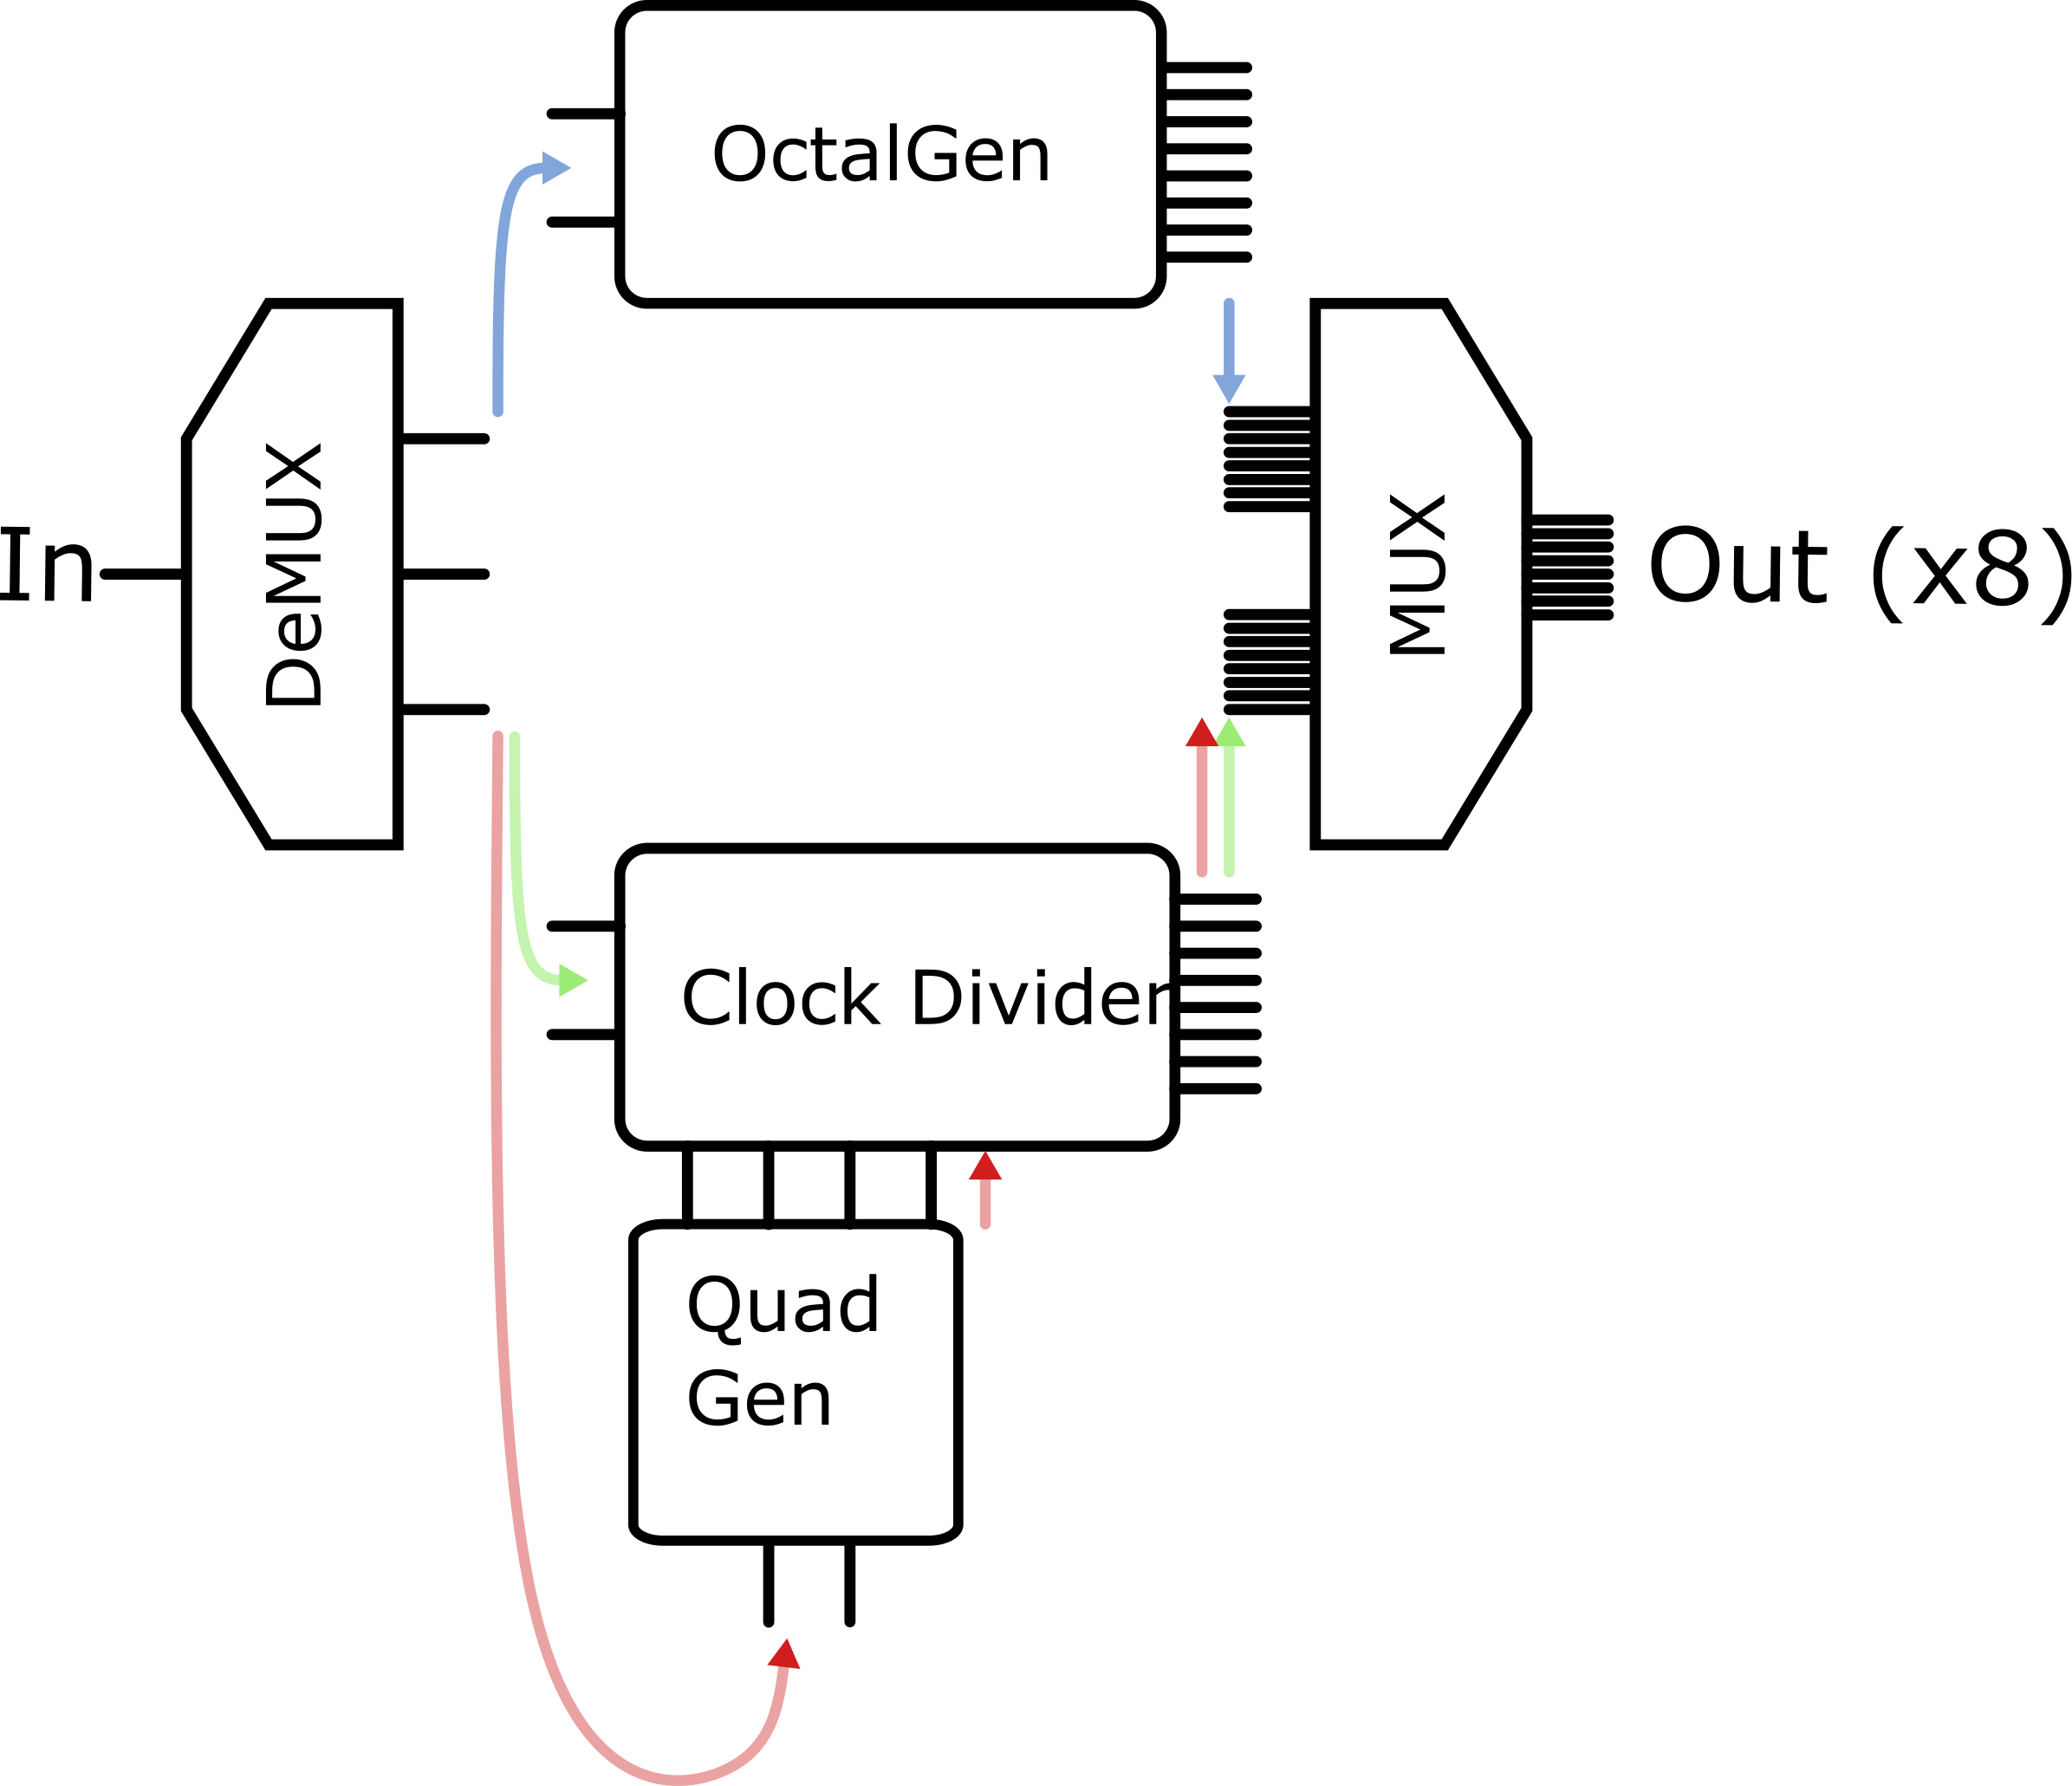
\includegraphics[width=0.8\linewidth]{figures/Schematics/mixF_design.png}
  \caption{Final design architecture with three frequency paths: High-Frequency (HF), Mid-Frequency (MF), and Low-Frequency (LF). The input demultiplexer selects the operational mode, while the output multiplexer combines the outputs from the HF and MF/LF paths.}
  \label{fig:mixF_design}
\end{figure}

An output 2:1 multiplexer selects between the HF and the combined MF/LF output, providing an additional layer of isolation to reduce noise and lower jitter. For design efficiency, the fine-tuning Current-Starved Inverters (CSIs) were placed at the very end of the signal chain, after the output multiplexer. This strategic placement allows a single set of CSIs to correct for skew introduced by all preceding logic, including the input demultiplexer and the main delay stages, regardless of the selected frequency mode.

To further enhance performance, cross-coupling was strategically introduced at critical nodes to improve signal slew rates and guarantee accurate phase spacing.

In subsequent design testbenches, the finetuner was disabled, since the focus was on verifying the functionality of the main delay stages and the ability to produce the clock phases across frequencies and corners with a coarse tuning loop.

\subsection*{Input Demultiplexer and Output Multiplexer Designs}\label{sec:demux_mux_design}

The input demultiplexer and output multiplexer were designed to meet the stringent requirements of the clock generator, namely low jitter, high input-to-output isolation, and minimal area overhead. The input demultiplexer selects where to send the two input clocks, either to the high-, mid- or low-frequency path. The output multiplexer selects between the high-frequency output or the combined mid- and low-frequency outputs that subsequently get fed into the fine-tuning stage.

\subsection{Input Demultiplexer}

The input demultiplexer was constructed using a two‑stage buffer design, where the first stage consists of two identical regular tristate inverters and the second stage is a common‑source inverter stage. PMOS/NMOS common‑gate transistors pull the intermediate networks to \texttt{AVCC}/\texttt{GND}, respectively. An enable signal controls the tristate inverters and the intermediate‑node pull‑up/down networks.

The schematic of the input demultiplexer is shown in Figure~\ref{fig:input_demux}. As an input disturbance arrives at the input, a small fraction of the signal flows through \(C_{\text{in}}\) to the intermediate node. Most of this current flows through the pull-up/pull-down networks, since those transistors are enabled by the enable signal. Since the next stage's input load is likely large, the impedance of the low on resistance will be much lower compared to that of the output inverter's \(C_{\text{gd}}\) in series with the output load capacitance. Moreover, any disturbance at the intermediate node will cause an output voltage roughly given by \(V_{\text{out}} \approx \frac{V_{\text{int}}\cdot C_{\text{gd}}}{C_{\text{gd}} + C_{\text{out}}}\). Assuming \(C_{\text{gd}} \ll C_{\text{out}}\), the output voltage swing will be very small.

\begin{figure}[H]
  \centering
  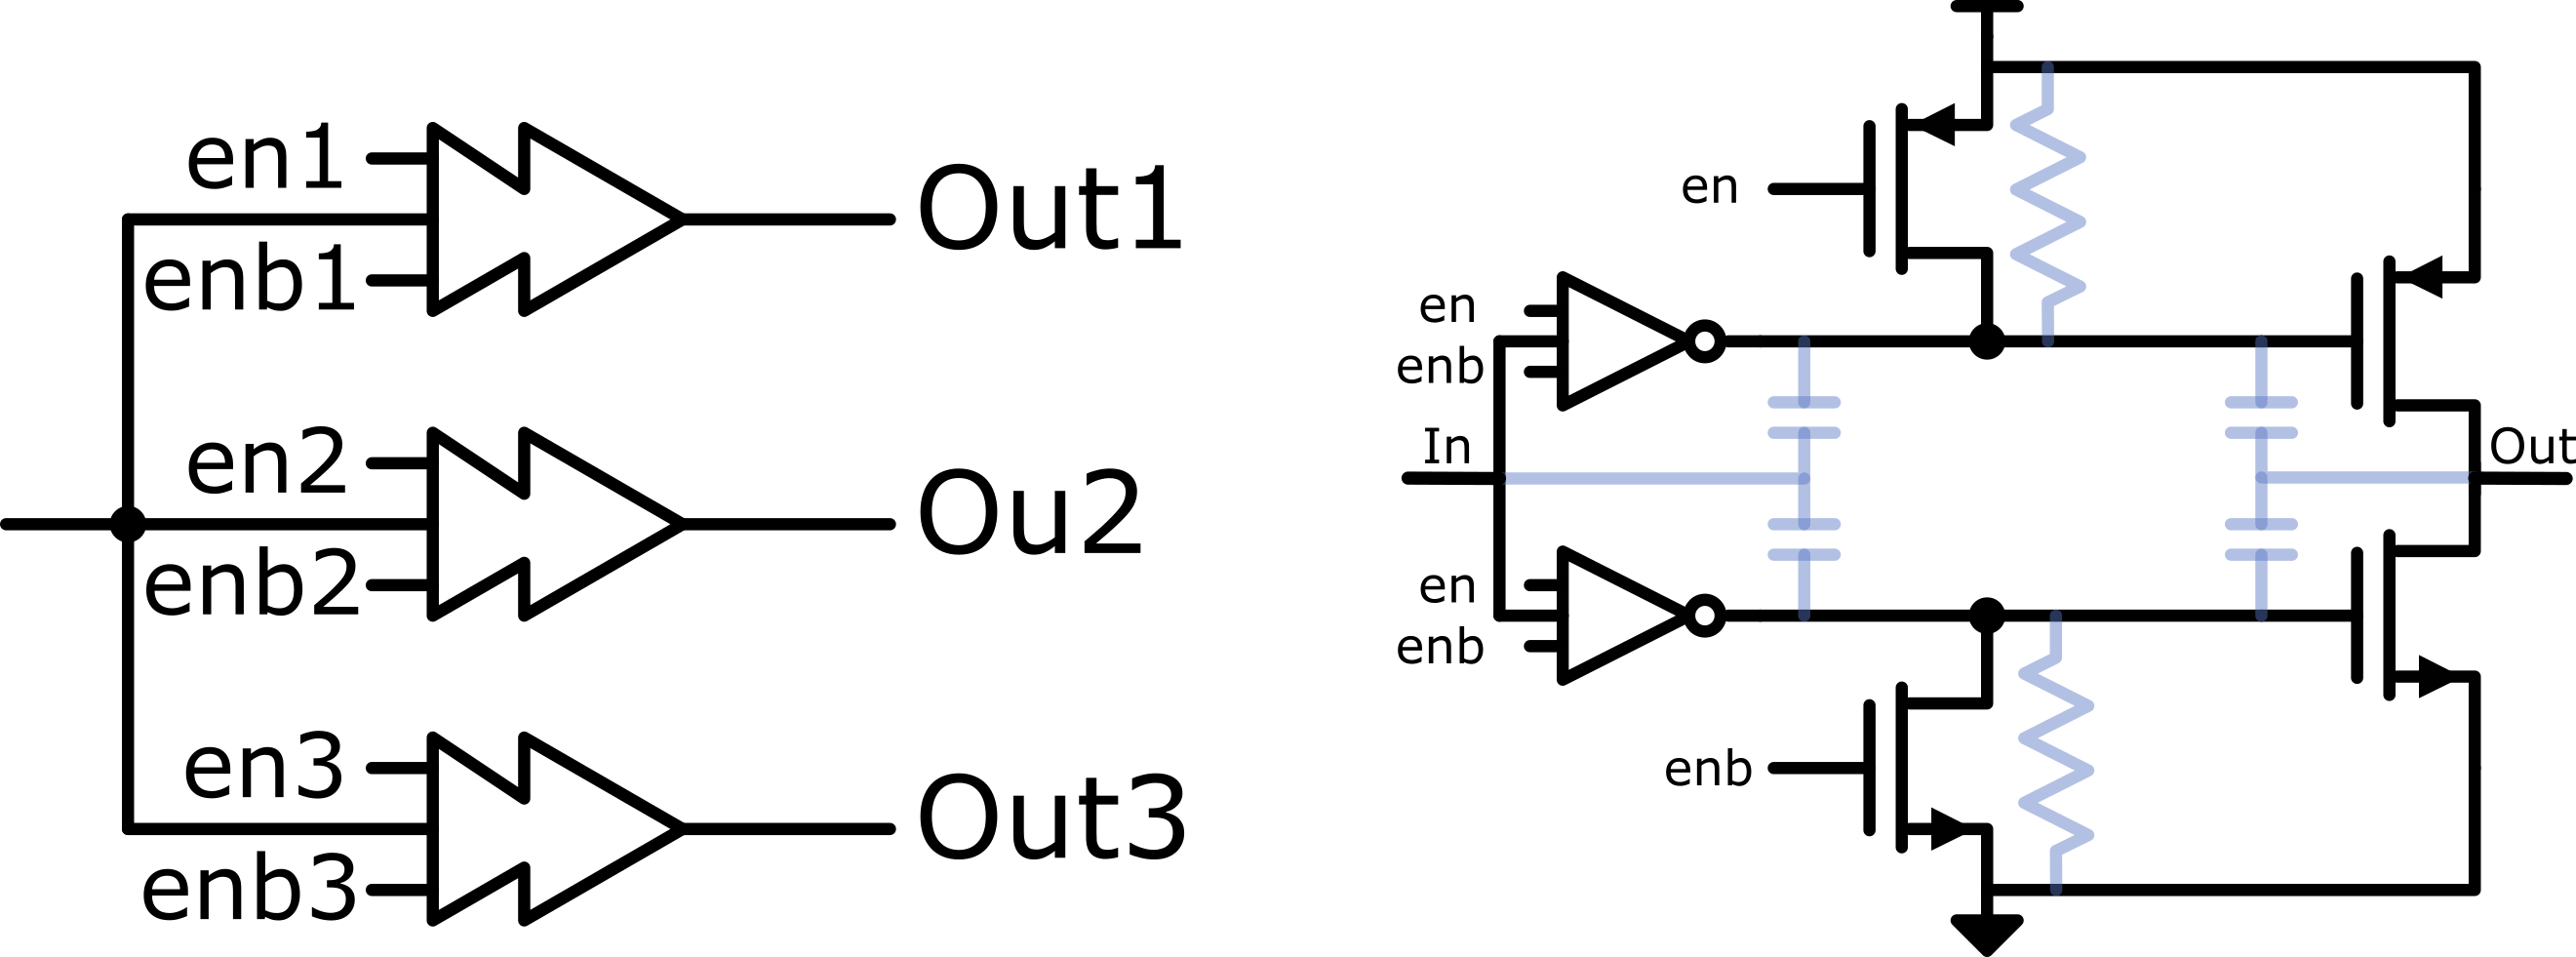
\includegraphics[width=0.8\linewidth]{figures/Schematics/input_demux.png}
  \caption{Input demultiplexer schematic. The first stage consists of two identical tristate inverters, while the second stage is a common-source inverter stage. PMOS/NMOS common-gate transistors pull the intermediate networks to \texttt{AVCC}/\texttt{GND}, respectively.}
  \label{fig:input_demux}
\end{figure}

It is also important to note that since the intermediate nodes are close to the rail voltage, the output transistors are biased in the cutoff region and small voltage changes below \(V_\text{th}\) at the gate will not result in \(I_\text{DS}\) at the output.

\subsection{Output Demultiplexer}

The schematic of the output multiplexer is shown in Figure~\ref{fig:output_mux}. The design uses a two simple TGate switches to select between the high-frequency and mid/low-frequency outputs.
A 2-bit control signal selects which switch to close, allowing one of the two inputs to be connected to the output. The TGate switches are designed to minimize introduced jitter and ensure adequate isolation between the two output paths. The TGate switches are also sized to have low on-resistance, minimizing voltage drop across the switch and ensuring that the output signal remains close to the rail voltage.

\begin{figure}[H]
  \centering
  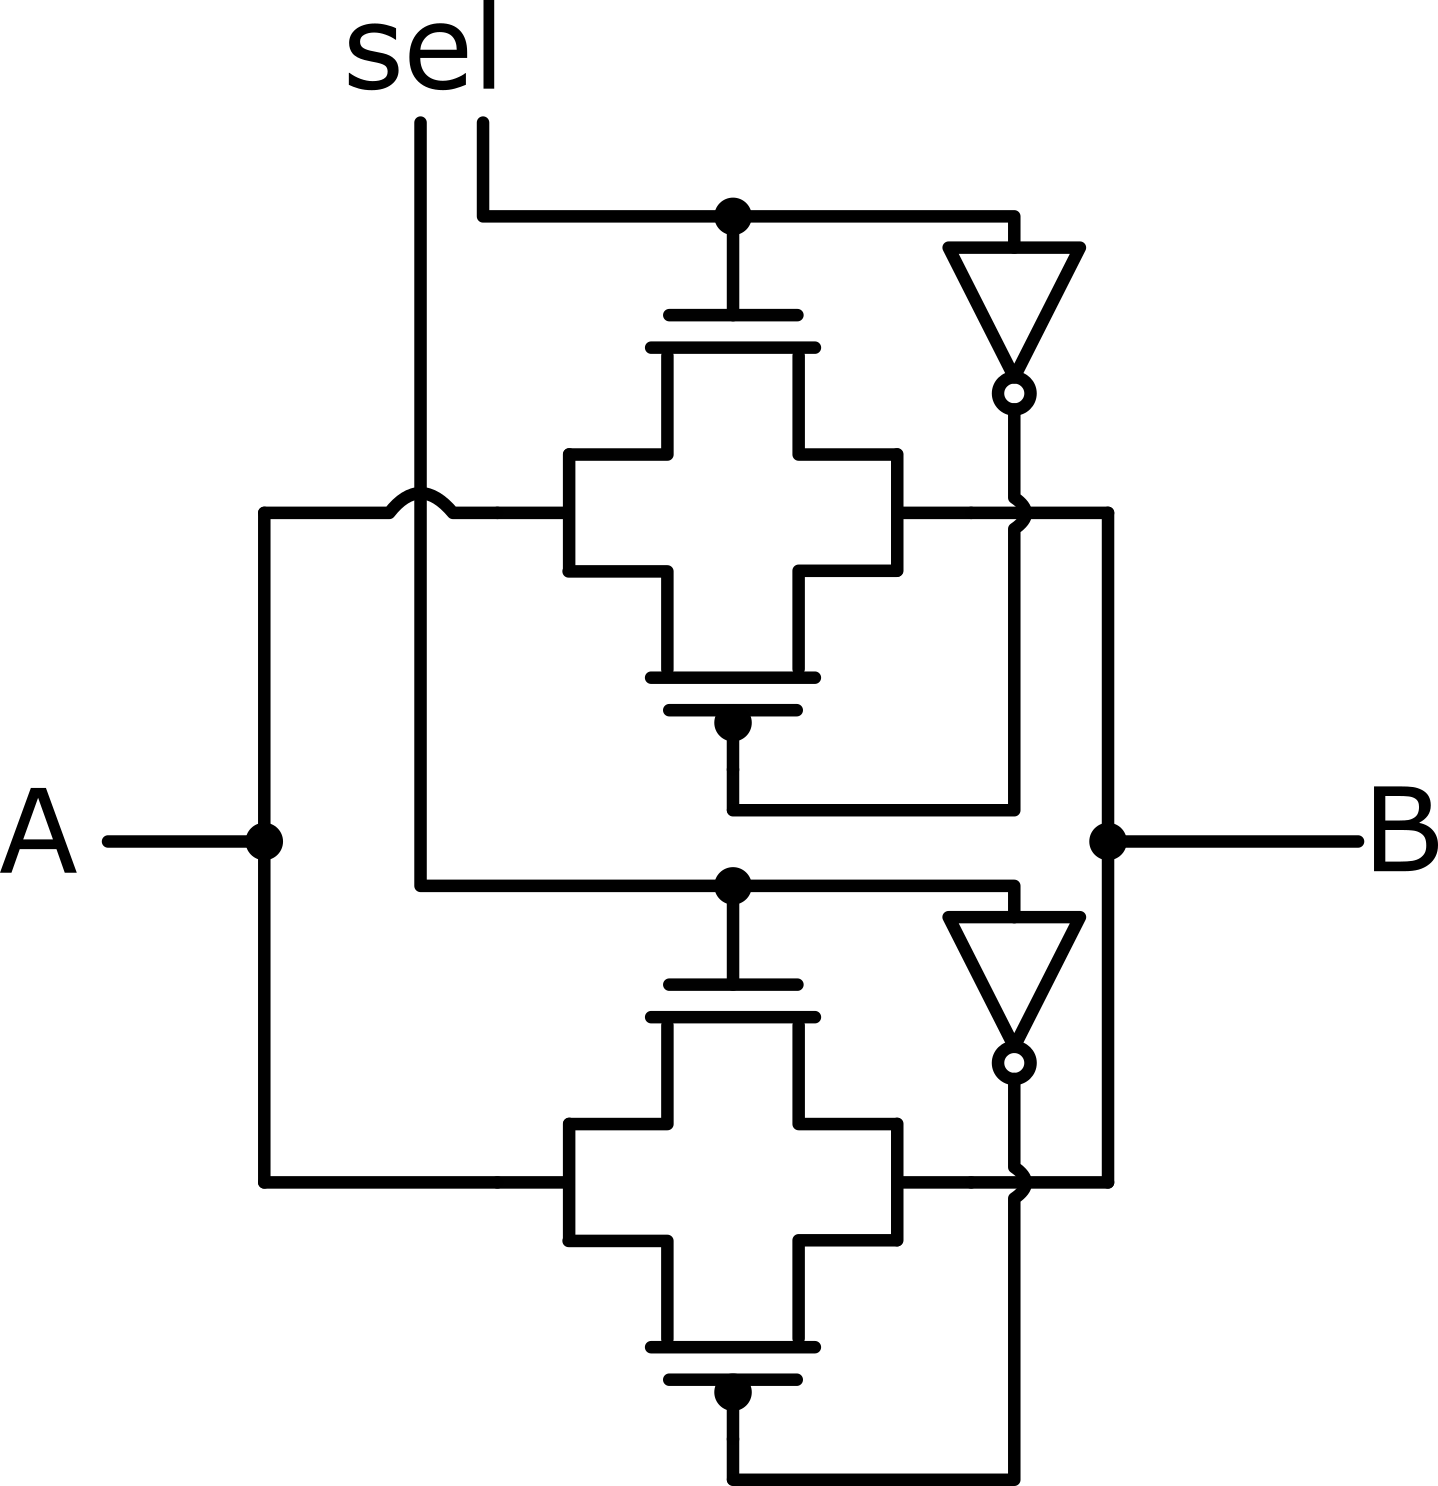
\includegraphics[width=0.3\linewidth]{figures/Schematics/output_mux.png}
  \caption{Output multiplexer schematic. The design uses two TGate switches to select between the high-frequency and mid/low-frequency outputs. A 2-bit control signal selects which switch to close, allowing one of the two inputs to be connected to the output.}
  \label{fig:output_mux}
\end{figure}


\subsection{Octal- and Quad-Generator Designs}\label{sec:octal_quad_gen_design}

The Octal-Generator (OctalGen) was implemented as the pure delay line design described in Section \ref{sec:second_redesign}, with eight independent delay paths generating the eight output phases. Each path consists of a series of programmable delay elements implemented through capacitive DACs. The OctalGen is designed to operate at high frequencies, with the ability to generate clock phases from 11GHz to 22.5GHz. 

The Quad-Generator (QuadGen) is used in the MF mode and was implemented as half of the OctalGen, generating four output phases at the same frequencies and following the exact same design. Importantly, The four output phases are divided once by two using half of the clock divider circuit which will be described below. This frequency division implies the MF path outputs eight phases at half the frequency of the HF path, allowing the design to operate at frequencies down to 5.625GHz. Below such frequencies, the LF path is used.

A key consideration in MF mode is the phase spacing between the output clocks. The MF path generates four output clocks that are \ang{90} apart, which are then divided by two to produce eight output clocks that are \ang{45} apart. This implies that tuning phase \ang{90} and \ang{270} is sensed as a phase shift of \ang{45} at the output. All other phases are a consequence of the correct spacing between the four output clocks, meaning accurate tuning is achieved by sensing \ang{45} to tune the \ang{90} and \ang{270} phases. This adaptation was implemented as a Verilog-A block that routes the appropriate clock signal to the \ang{90} and \ang{270} CDAC control blocks, ensuring that the correct paths are adjusted for each mode of operation.

\subsection{Low-Frequency Path (Clock Divider) Designs}

The low-frequency path is implemented using a two-stage clock divider composed of flip-flops.

Between the first and second stages, a 2:1 multiplexer selects between the output of the first LF stage and the output of the MF path, allowing the latter to operate at half the frequency of the HF path. This multiplexer is controlled by a simple digital control signal that closes one of two TGate switches, connecting either the first stage output or the MF path output to the second stage.

The first stage divides the input clock by two, generating four output clocks at half the input frequency. The second stage further divides these clocks by two, resulting in eight output clocks at a quarter of the input frequency when in LF mode.

In pure LF, there are no addressable skew modulators, since assuming the input clocks are correctly spaced, the output clocks will be perfectly spaced owing to the fully-differential chains and the cross-coupling inverters introduced along the chain. The main design challenges in the LF path were ensuring reliable operation by avoiding metastability and meeting timing requirements across process corners to prevent skipping clock cycles, especially on startup.

\subsubsection{2-stage Divider Design Employing Parallel Flip-Flops}
The schematic of the first implementation for the 2-stage divider is shown in Figure~\ref{fig:2stage_divider}.
This first implementation of the LF path was built for simplicity and robustness, using two identical stages of differential flip-flops arranged in parallel. The first stage consists of two flip-flops, each toggling on the rising edge of one of the input clocks (\(0_{\text{in}}\) and \({180}_{\text{in}}\)). The second stage consists of four identical flip-flops, each sampling one of the output clocks driven by the first stage (\(0_{\text{mid}}\), \(90_{\text{mid}}\), \(180_{\text{mid}}\) and \(270_{\text{mid}}\)). This design ensures that there is enough timing margin for the data input of any flip-flop to settle before the arrival of the next clock rising edge, avoiding metastability and guaranteeing that the output clocks are correctly sequenced. 

\begin{figure}[H]
  \centering
  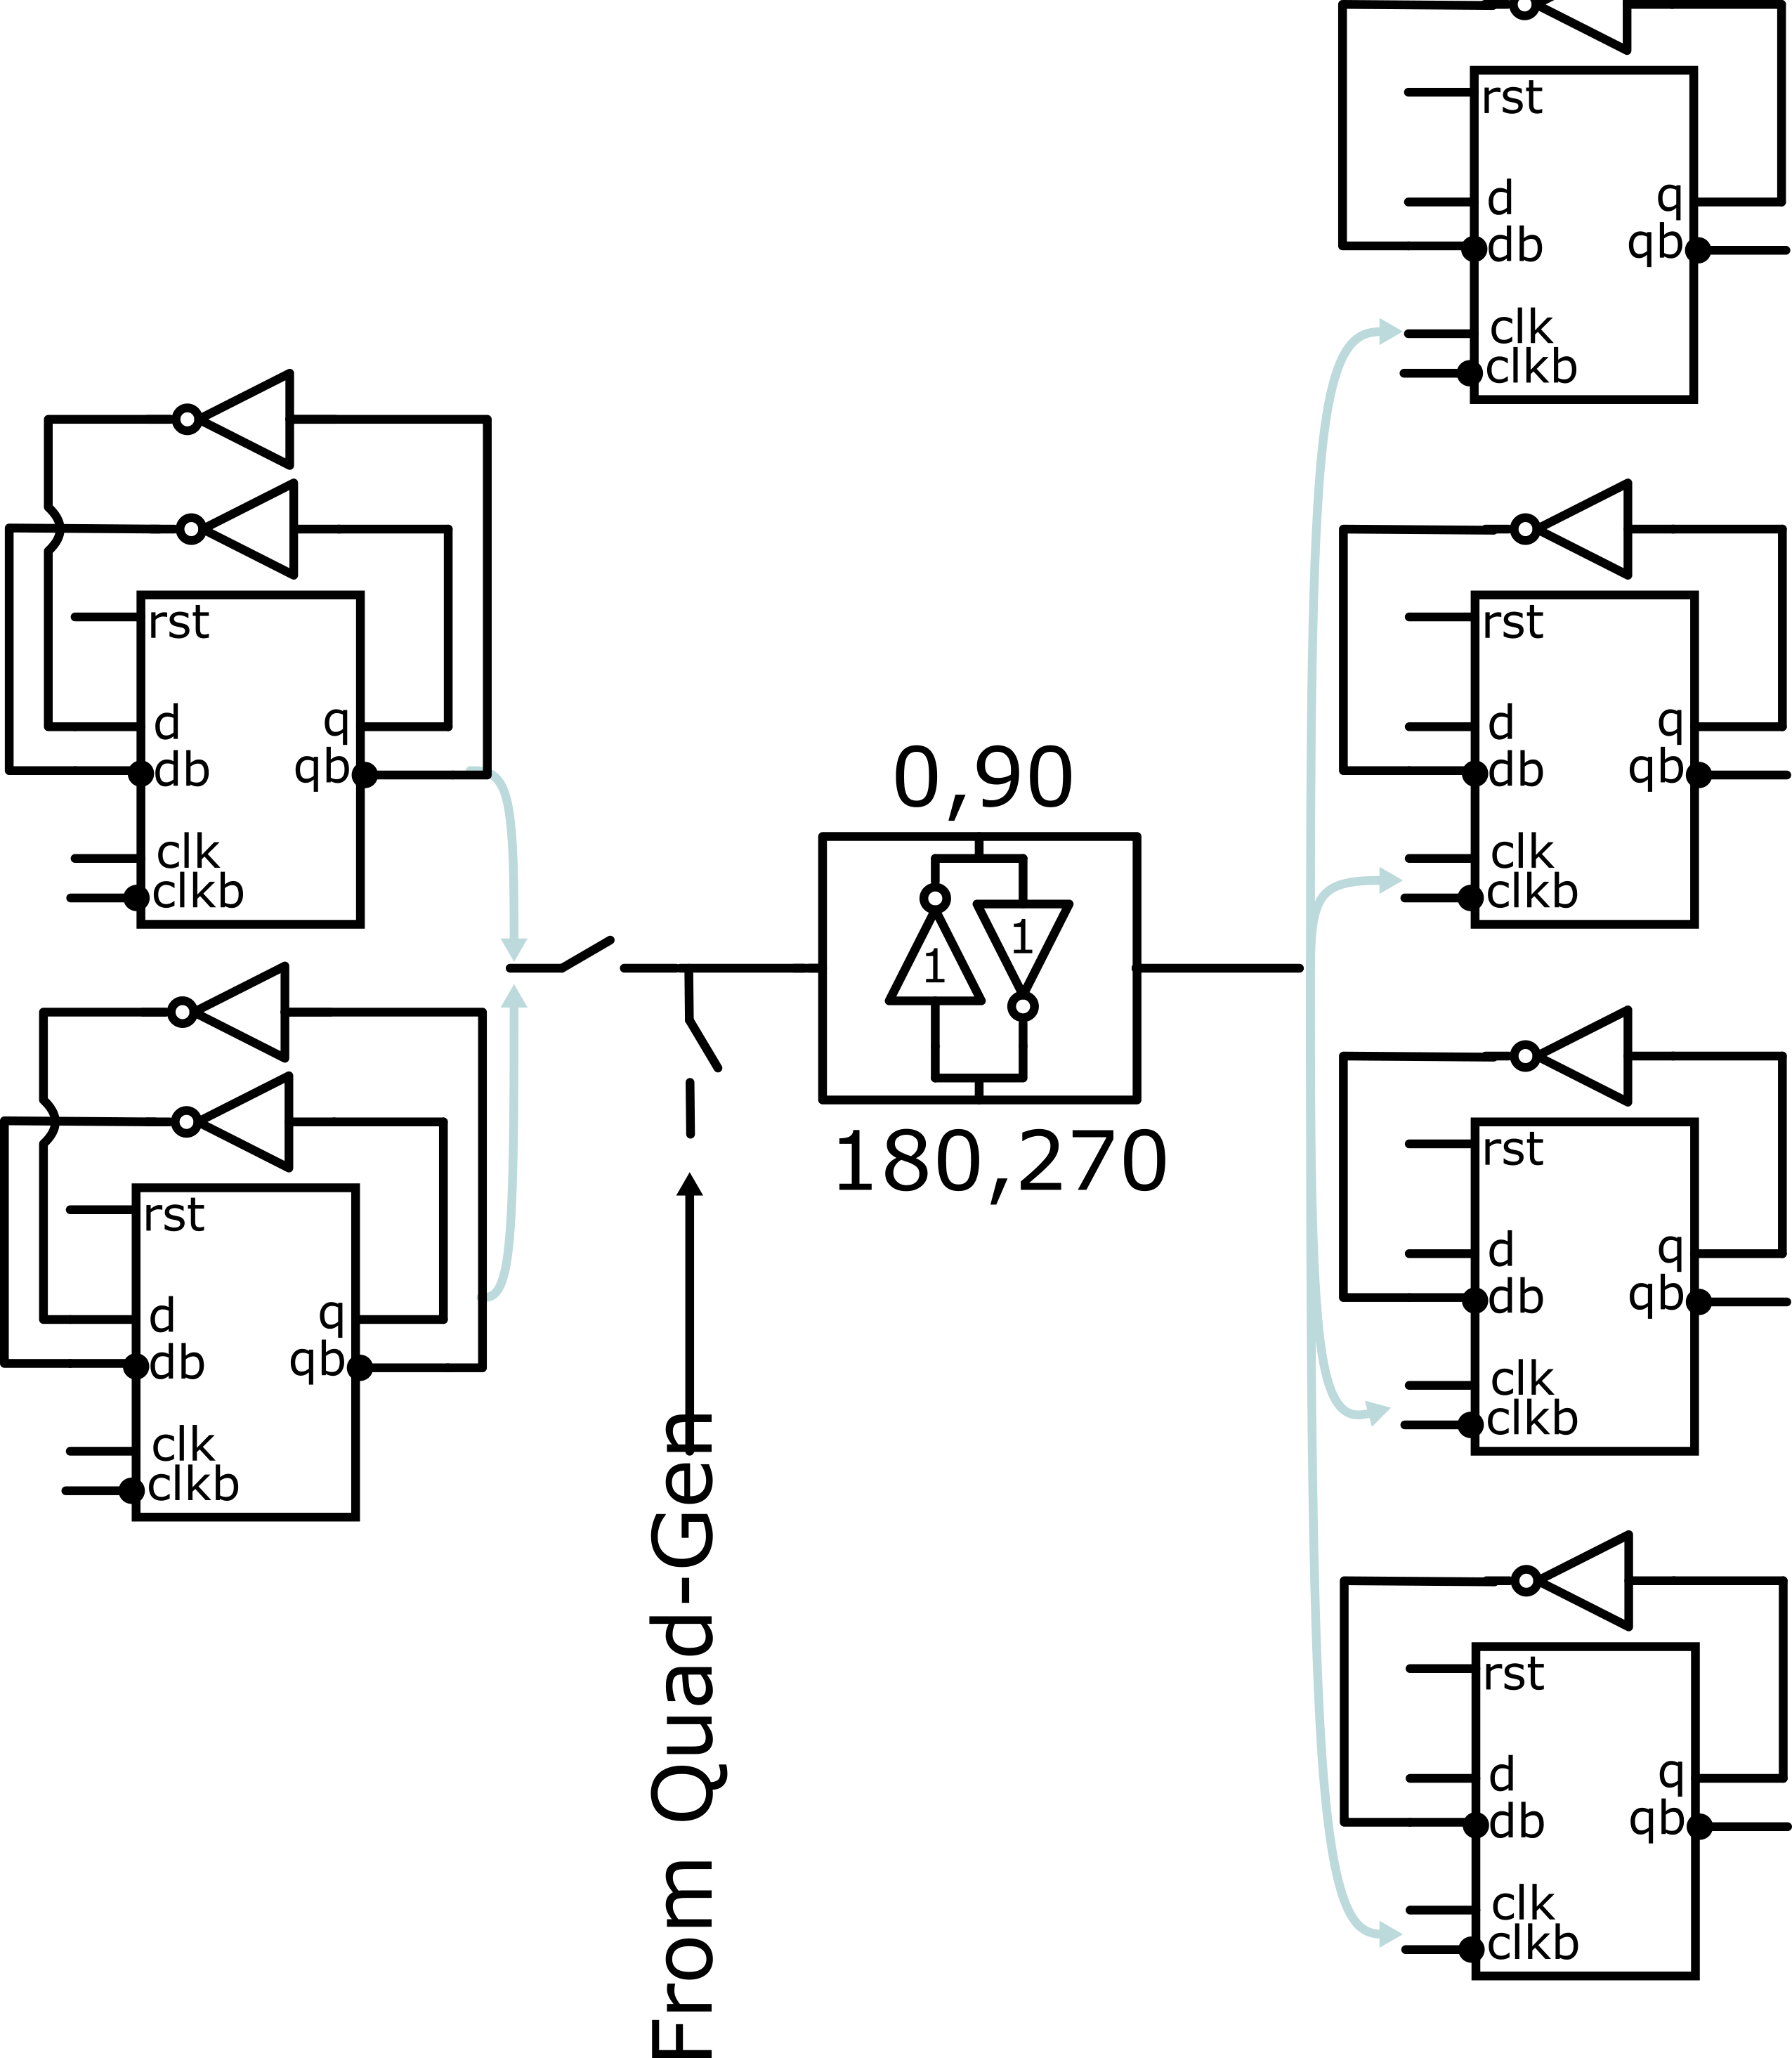
\includegraphics[width=0.8\linewidth]{figures/Schematics/2stage_divider.png}
  \caption{Schematic of the first implementation of the 2-stage clock divider. The first stage consists of two flip-flops, while the second stage consists of four flip-flops sampling the output clocks from the first stage.}
  \label{fig:2stage_divider}
\end{figure}


\paragraph{Reset Sequence and Logic:}

A critical aspect of the first divider design highlighted above is the reset sequence. Without a proper sequential reset, the flip-flops in the divider circuits can initialize at random states, leading to unpredictable output clock phases, even if relative shifts remain correct. To prevent this, a robust reset sequence was implemented.

The main challenge lay in the fact that, in MF, the reset occurs before the QuadGen is fully tuned, meaning the phase spacing between adjacent clocks (e.g., \ang{0} and \ang{90}) might be too small for cascaded flip-flops to sample correctly. To solve this, the reset sequence is initiated using clocks that are guaranteed to be well-separated. 

In LF mode, the reset is globally triggered by clock \ang{180} from the input, while in MF mode, it is triggered by clock \ang{270} from the quad-generator output. 

Cascaded flip-flops are subsequently arranged in such a way to guarantee that two consecutive flip-flops are clocked by clocks that are at least \ang{180} apart, ensuring settling before sampling. The final arrangement is shown in Figure~\ref{fig:reset_seq}, where the consecutive samplings eventually generate the sequential reset signals after three stages.

\begin{figure}[H]
  \centering
  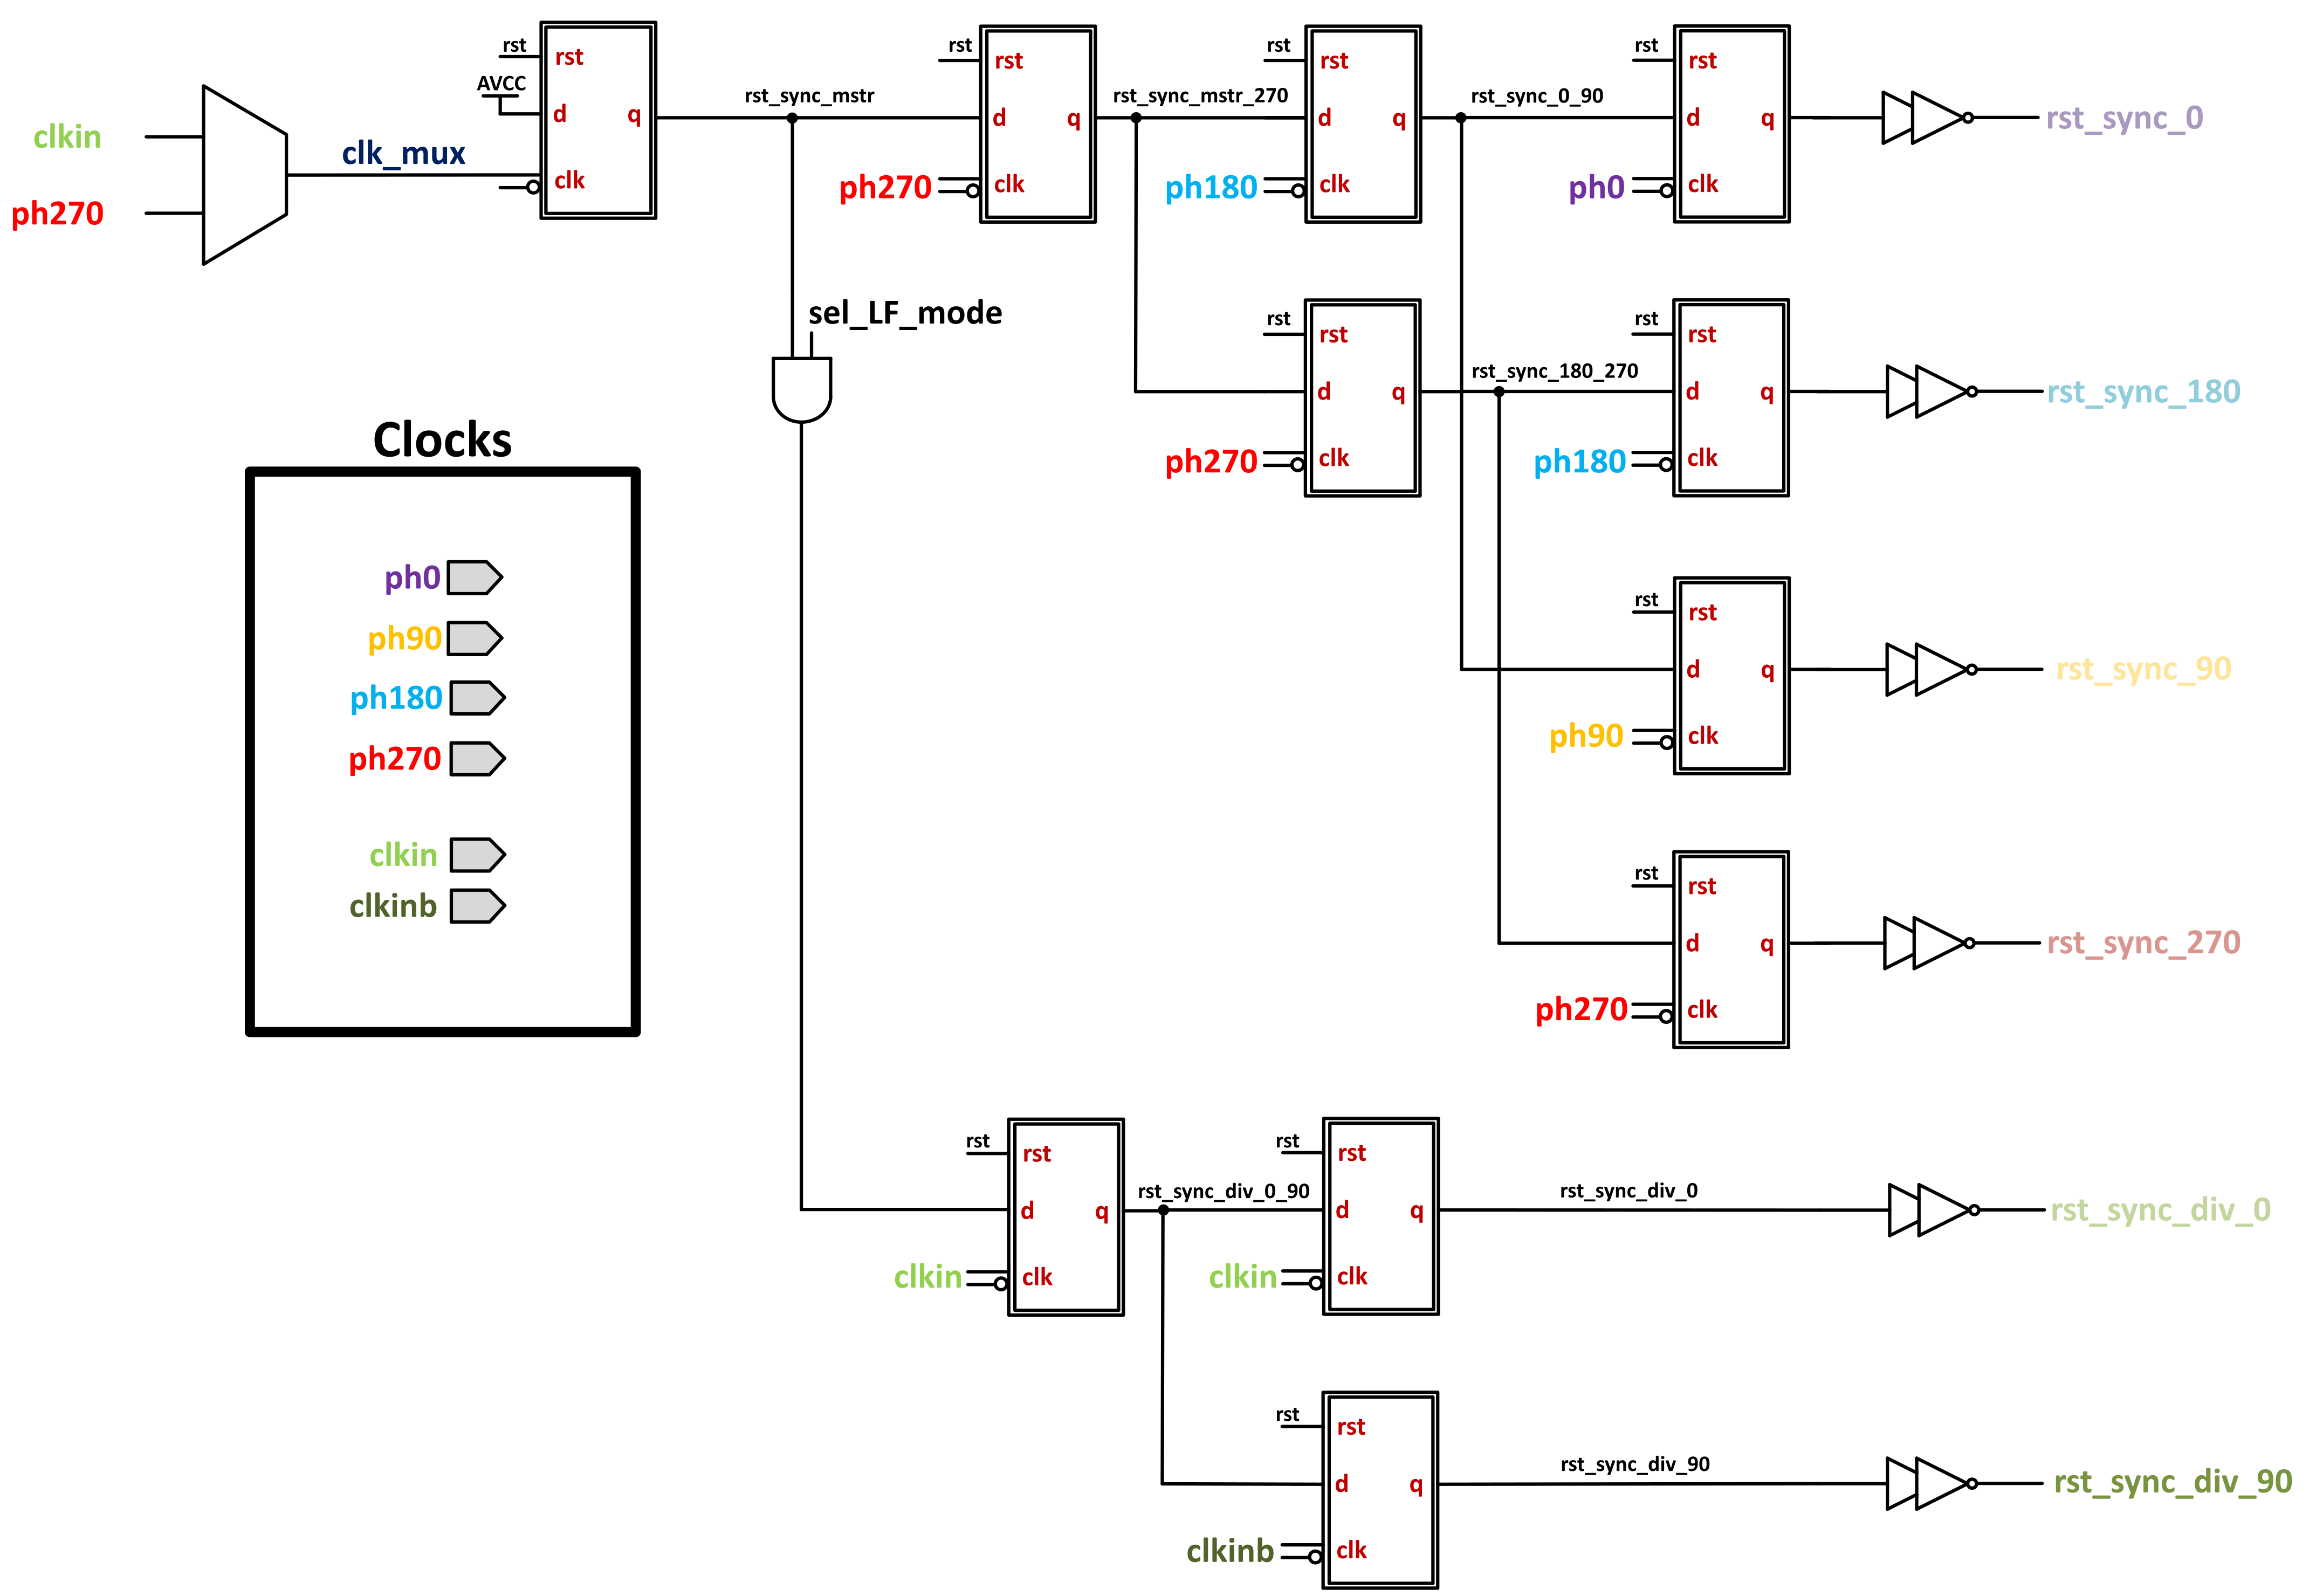
\includegraphics[width=\linewidth]{figures/Schematics/reset_seq.png}
  \caption{Reset sequence logic for the 2-stage clock divider. The reset is triggered by clock \ang{180} in LF mode and clock \ang{270} in MF mode, ensuring that consecutive flip-flops are clocked by clocks that are at least \ang{180} apart.}
  \label{fig:reset_seq}
\end{figure}


\subsubsection{V2 - 2-Stage "Ring-Oscillator"-like Divider With Clock Slip}
In an attempt to design a reset-free clock divider, a second implementation of the 2-stage clock divider was developed. This design is based on a ring-oscillator-like structure. The schematic of this second implementation is shown in Figure~\ref{fig:div_V2_complete}. 
Setting aside the clock slip and synchronizer, the first stage consists of a single fed-back flip-flop, which samples the input clock and feeds it back to its own data input. The output of this flip-flop is subsequently fed into a set of two flip-flops, clocked at \ang{0} and \ang{180}, leading to the generation of four correctly-spaced output clocks at \ang{0}, \ang{90}, \ang{180} and \ang{270} oscillating at half the input frequency. 
Since the data input of both flip-flops is driven by the same input, the output clocks are guaranteed to be follow the expected \(0\rightarrow 90\rightarrow 180\rightarrow 270\) sequence.
The second clock division stage consists of four cascaded flip-flops, clocked at \ang{180}, \ang{270}, \ang{0} and \ang{90} sequentially along the chain, with the output of the latter stage feeding back into the first stage's data input. This structure guarantees that the output clocks are likewise correctly sequenced.

\paragraph{Clock Slip and Synchronizer:}
Rate-matching between a SerDes transmitter and reciever chain is a common challenge and in some instances perfect frequency alignment is not possible. To address this, a clock slip mechanism is implemented in the clock generator. This mechanism allows the clock divider to slip by one clock cycle, halting data transfer temporarily.

Supposing the transmission chain is running at a slightly higher frequency than the receiver chain, the clock slip mechanism allows the receiver to catch up by skipping a clock cycle. 

In the present design, the clock slip mechanism is implemented using a TGate switch connecting the input and output of the feedback inverter in the first stage, while simultaneously disconnecting the inverting common-source inverters from the output (shown in Figure~\ref{fig:div_V2_complete}). This stops the intermediate node in the first stage from toggling, halting the clock generation.

The enable signal for toggling the TGate switch must be generated with very good precision such that exactly one period is skipped. This is achieved by using a synchronizer, drawn in Figure~\ref{fig:sync}.

The clock slip enable is asynchronous, simplifying the logic but greatly increasing the risk of metastability. 

To mitigate this, an \texttt{en\_clkslip} signal is generated moments before the clock slip is triggered. This turns on a divide-by-eight chain whose output clocks a set of four cascaded flip-flops. 

The purpose of dividing the clock by eight is to reduce the risk of switching \texttt{pcd\_2UI} (second control signal for the clock slip that actually decides when to slip) too close to a clock edge. This reduces the total number of edges per unit time, which could otherwise lead to metastability due to insufficient timing margin between the data input and clock signal. 

Moreover, the four chained flip-flops have a very high chance of resolving metastability, should it still occur at the first stage. \texttt{pcd\_2UI} must have a total high time of at least eight clock cycles, which guarantees sampling at one edge of the divide-by-eight chain.
This mechanism ensures the \texttt{synced} signal is stable and transitions at a clock rising edge.

As shown in Figure~\ref{fig:div_V2_complete}, the \texttt{synced} signal is the data input of a two-stage flip-flop synchronizer, with the differential outputs of both stages feeding into a fully-differential XOR gate.
After \texttt{synced} rises, the next rising edge of the clock will trigger the first stage of the synchronizer, which will transition the output to high. The second stage will remain low for exactly one clock period, after which it will transition to high. During this intermediate time, exactly one clock cycle, the XOR gate will output a high signal, which is used to enable the TGate switch in the first stage of the clock divider, triggering the clock slip mechanism.

\begin{figure}[H]
  \centering
  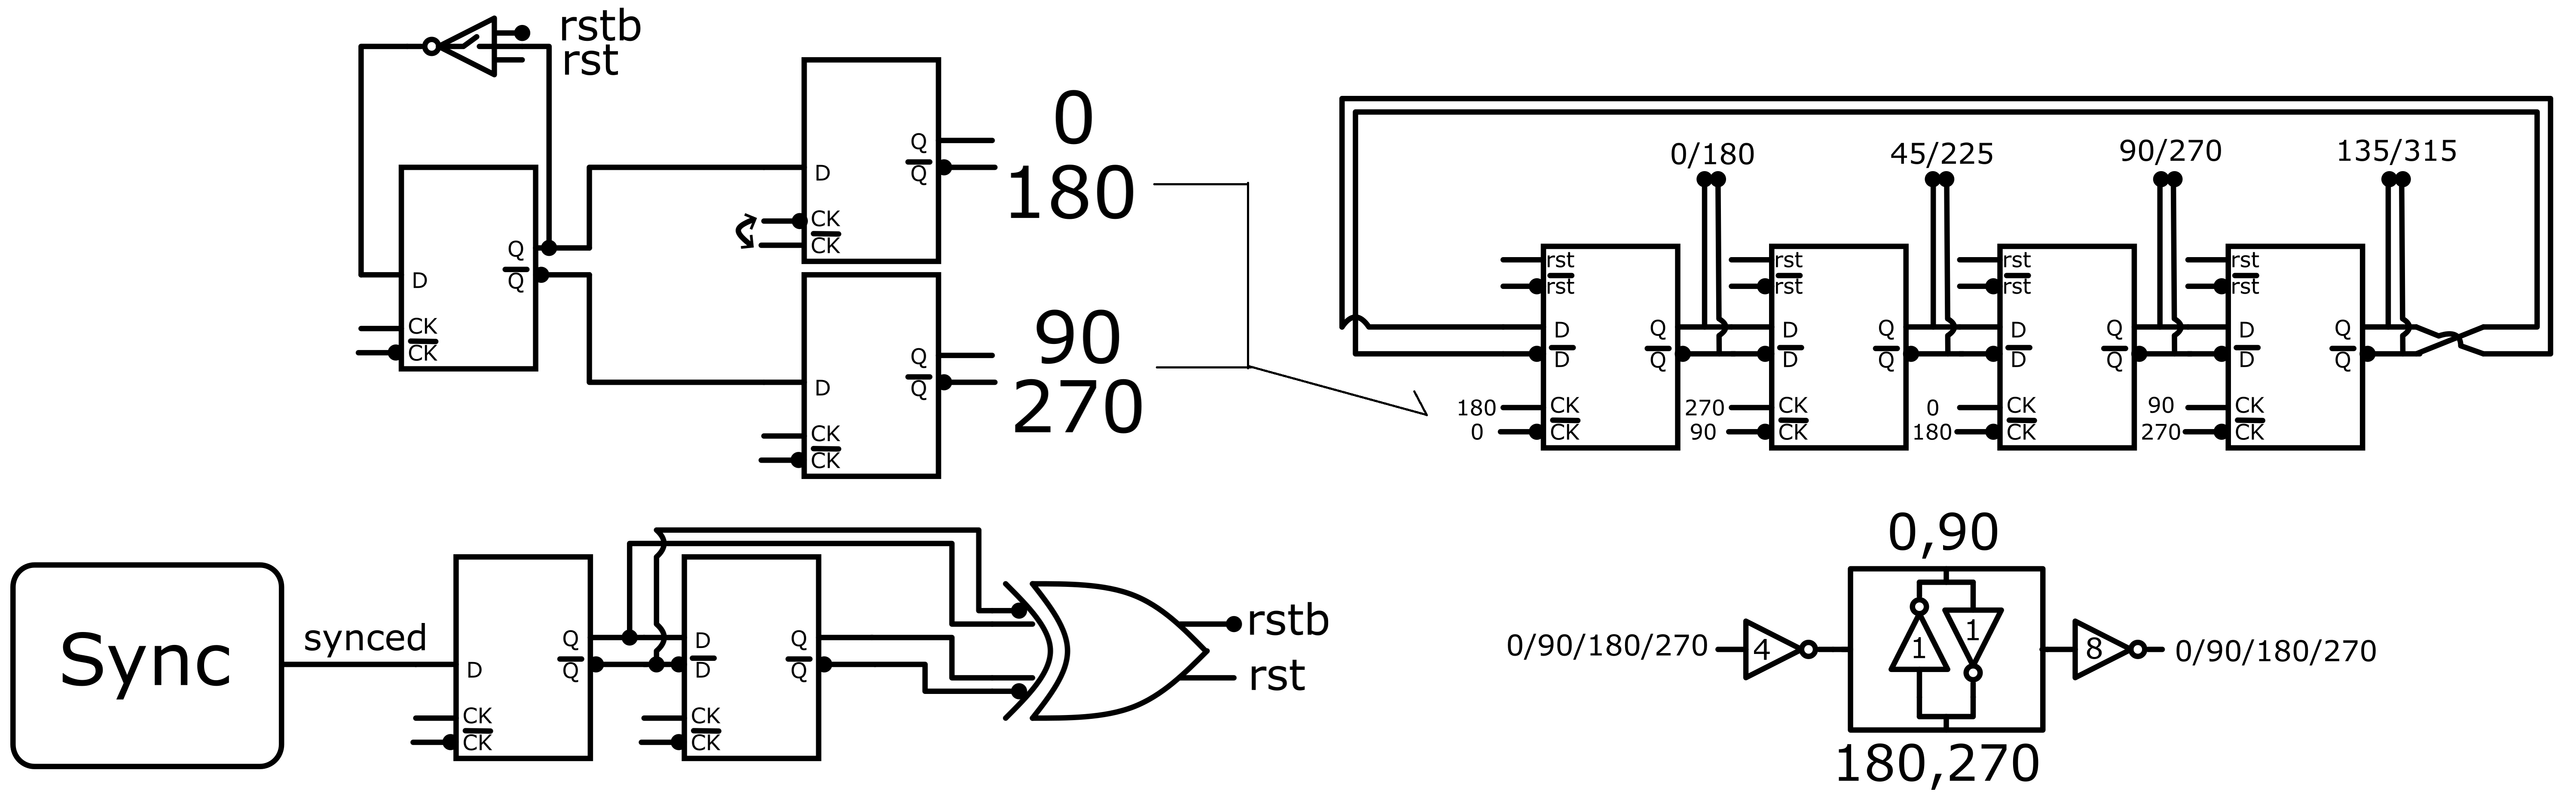
\includegraphics[width=\linewidth]{figures/Schematics/div_V2_complete.png}
  \caption{Schematic of the second implementation of the 2-stage clock divider, based on a ring-oscillator-like structure. The first stage consists of a single fed-back flip-flop, while the second stage consists of four cascaded flip-flops.}
  \label{fig:div_V2_complete}
\end{figure}
\begin{figure}[H]
  \centering
  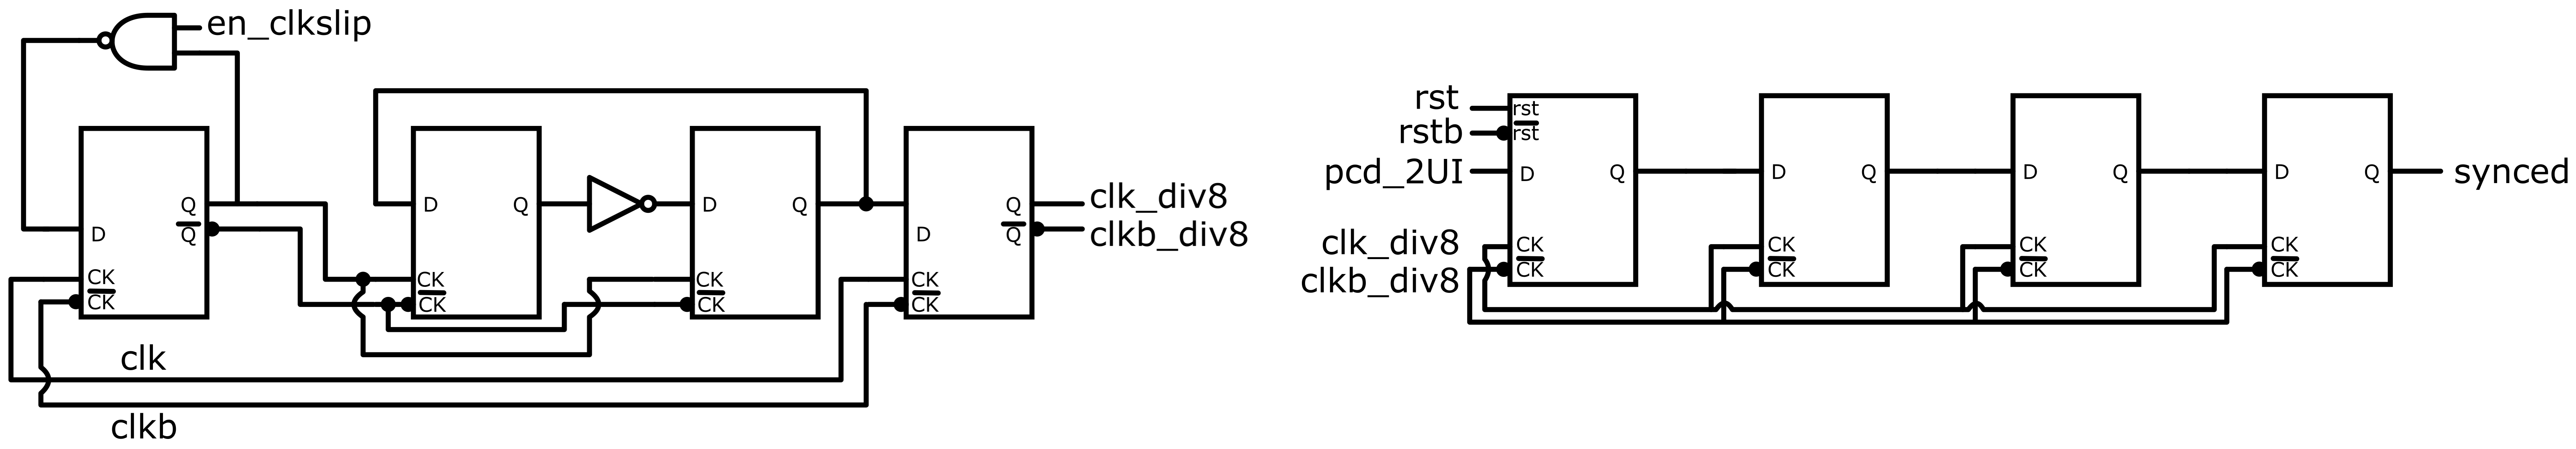
\includegraphics[width=\linewidth]{figures/Schematics/sync_complete.png}
  \caption{Schematic of the clock slip synchronizer. The synchronizer ensures that the clock slip mechanism is triggered with very good precision, allowing exactly one period to be skipped.}
  \label{fig:sync}
\end{figure}

\subsection{Output Fine‑Tuning by Phase Interpolation}\label{sec:output_finetuning}

The final stage of the multiphase generator (MPG) is dedicated to trimming the output clock phases. Capacitance banks were originally intended to remain dynamically programmable so that temperature‑induced drifts could be cancelled in real time. Stress simulations, however, revealed that toggling the most‑significant bit (MSB) of a bank introduces a transient disturbance: the duty cycle and propagation delay deviate for one—and occasionally two—clock cycles before converging. Although this behaviour did not violate timing in process–voltage–temperature (PVT) corner simulations with the Verilog‑A delay‑compensation wrapper enabled, its magnitude warranted mitigation.

\paragraph{Capacitance‑bank timing study.} Figure~\ref{fig:dcd_MSB} shows the duty‑cycle distortion recorded while forcing an MSB transition at incremental offsets within the clock period. Because each branch carries a phase‑shifted replica of the master clock, simultaneously switching every bank at the ‘optimal’ instant is impossible without per‑branch timing control, additional routing, and removal of the cross‑coupling latches that suppress jitter. Thermometer‑coding the MSBs, which reduces the incremental capacitance step, alleviated the glitch in schematic experiments but increases area and control complexity. We therefore turned to a digital phase interpolator (PI) that can operate continuously while the banks are parked at a safe static code.

\paragraph{Phase‑interpolator architectures.} A tri‑state‑inverter PI from an earlier revision provided a convenient starting point: two quadrature input clocks drive parallel tri‑state inverters; enabling/disabling the inverters weights the contribution of each input and hence skews the output phase. Two variants were implemented (Fig.~\ref{fig:phase_interpolators}):
\begin{enumerate}
\item \textbf{Three‑path PI} — independent tri‑state banks fed by clocks at \ang{0}, \ang{45}, and \ang{90}.
\item \textbf{Two‑path PI} — one bank driven by the fixed \ang{45} clock; the second is multiplexed between \ang{0} and \ang{90}.
\end{enumerate}
The three‑path topology promises superior linearity but imposes a larger capacitive load on the clock network and demands more control bits. The two‑path topology is both smaller and less intrusive.

\paragraph{Isolation improvement.} Under identical conditions at 22.5,GHz with seven binary control bits, both PIs exhibited nearly uniform phase steps. In the two‑path PI a single large step appeared during the MUX transition, traced to residual coupling through a disabled tri‑state inverter. Relocating the enable switch between the inverter pull devices and the output node improved isolation and removed the glitch. Converting the three MSBs to thermometer code further linearised the transfer and suppressed switching spikes.

\paragraph{Performance summary.} Table~\ref{tab:phase_interpolator_metrics} summarises the simulated results. The two architectures deliver comparable linearity and power, but their \textasciitilde43,fs average step still falls short of the specification. Future iterations will extend the control word by one or two bits to meet the required resolution without compromising jitter.

At this juncture the PI constitutes a credible fallback to the current‑starved‑inverter (CSI) fine‑tuner discussed in Section~\ref{sec:csi}. The PI offers a wide, highly linear range; the CSI trades range for finer resolution. Neither circuit has yet been integrated into the full transmitter chain—comprehensive assessment will await the first complete MPG silicon.

% \subsection{Output fine-tuning investigation using phase interpolation}\label{sec:output_finetuning}
% The final design of the PDE includes a last stage responsible for fine-tuning the output clock phases.
% Initially, it was considered that the capacitance banks would be able to switch during operation to correct for temperature drift. However, during stress testing, it was observed that the capacitance banks had the capability to cause detectable clock disturbances where after an MSB switch, the clock duty-cycle and delay would drift significantly over one or, less frequently, two clock cycles. This was not observed to cause significaqnt issues during PVT corner simulations with the current verilogA delay sensing block, but it was a significant enough issue that warranted investigating ways to mitigate it.

% The MSB switch was first forced at different times during the clock cycle, but it was found that the only way to avoid clock collapse on all branches would be to switch the control bits on different branches at different times, which would require a more complex control logic, more wiring and most importantly necessitate the removal of the cross-coupling stages, which was important for low-jitter. Figure~\ref{fig:dcd_MSB} plots the duty-cycle distortions as the MSB switches at different times across the clock period. The switching delay of the MSB against clock 0's rising edge was incremented after each switch during a continuous transient simulation to confirm that the distortion settles after few clock cycles. The complementary phases to those displayed in the figure naturally exhibit the same distortions, but with opposite polarity. It was observed that the duty-cycle distortion is most significant when the MSB switches closer to rising edges of the clock, but since all branches have phase-shifted versions of the same clock, it would be impossible to switch the MSB at the optimal time across all nodes of all branches without significant redesign.
% Another option was to use thermometer coding for the MSBs of the capacitance banks, which would allow for a more gradual change in capacitance. this proved effective in schematic simulations, but was set aside as a final option, since it was expected that it could be possible to park the control bits at a safe value before the transmission chain is fully operational and then use the fine-tuning circuit during operation to correct for temperature drift.

% The fine-tuning circuit could be implemented using a current-starved inverter, as described in Section \ref{sec:csi}, but this would require DAC controls and had limited resolution close to the range limits. 
% The previous implementation of this project had made use of a digitally-controlled phase interpolator to achieve the finely-tuned output clock phases across a wide delay range, where tristate inverters arranged in parallel were switched in/out of two input clock paths driven by two clocks \ang{90} apart, hereby controlling the relative strength of both mixing inputs and skewing the output towards the desired output phase. Upon resimulating this previous design, it was found that this mixing technique had very good linearity and could achieve fine resolution.

% Two digitally-controlled phase interpolators were tested, one employing three distinct clock paths \ang{0}, \ang{90} and \ang{45}, each driving a bank of tristate inverters, and the other employing two inverter banks, one of which driven by a multiplexer connected to either clock \ang{0} or \ang{90} and the other to the intermediary clock \ang{45}. Both schematics are shown in Figure~\ref{fig:phase_interpolators}. The code (and MUX) switching sequence for phase sqewing is depicted in Figure~XX. The 3-path design was suspected to be more linear, but the 2-path design was more compact and, crucially, loaded the mixing node less and had less devices connected to the clock path, likely introducing less jitter and necessitating weaker inverters. Moreover, the 2-path design required less control bits, which was a significant advantage in terms of area and power consumption.

% Testing the two designs under identical conditions, both designs behaved very similarly, with the 2-path design showing equal step sizes across codes, except for the intermediate mux switching instance, which caused a large step. It was hypothesized this was due to insufficient isolation provided by the tristate inverters, which still contributed to the output clock phase, even when disabled. 

% A slight change to the tristate inverters, where whe binary-controlled MOS switches were placed between the input common source transistors and the inverter output (instead of the previous design, where these placements were switched), was made to improve isolation. This change completely eliminated the large step, allowing the 2-path design to achieve a very linear response across codes.

% As a last improvement, the three most sigmanificant bits (MSBs) were converted to thermometer coding, which allowed for a more linear response with little transient spikes during switching. 

% The final design of both designs was tested in a transient simulation, where the codes were gradually incremented across the full scale. The key metrics achieved by both implementations at 22.5~GHz with 7 binary control bits,  are succinctly summarized in Table~\ref{tab:phase_interpolator_metrics}. Both designs generally achieved similar performance, however, the resolution was still insufficient, indicating the final design would need one or more additional bits to achieve the desired resolution. This is expected to be addressed in future revisions of the design, where the fine-tuning circuit will be redesigned to achieve better resolution and lower jitter. 

% At this stage, the PI finetuning circuit was deemed sufficiently investigated and submitted as a secondary option to the previous CSI finetuning circuit. The main attraction of the PI design was its ability to achieve linear phase shifts across the full range, while the CSI design had a limited range but more resolution.

% Neither design was presently implemented in the final transmission chain as a final design choice, since more extensive testing would need to be performed by implementing the complete MPG design in a full chain, to correctly assess real performance and shortcomings.


\begin{table}[h]
\centering
\caption{Comparison of key metrics for 2- and 3-path PI finetuning implementations at 22.5~GHz.}
\begin{tabular}{|l|c|c|}
\hline
\textbf{Metric} & \textbf{3-path Implementation} & \textbf{2-path Implementation} \\
\hline
Minimum step (s) & 0 & 0 \\
Maximum step (s) & 68.96f & 71.61f \\
Average step (s) & 42.92f & 43.06f \\
Average power (W) & 4.675m & 4.481m \\
\hline
\end{tabular}
\label{tab:phase_interpolator_metrics}
\end{table}


\begin{figure}[H]
  \centering
  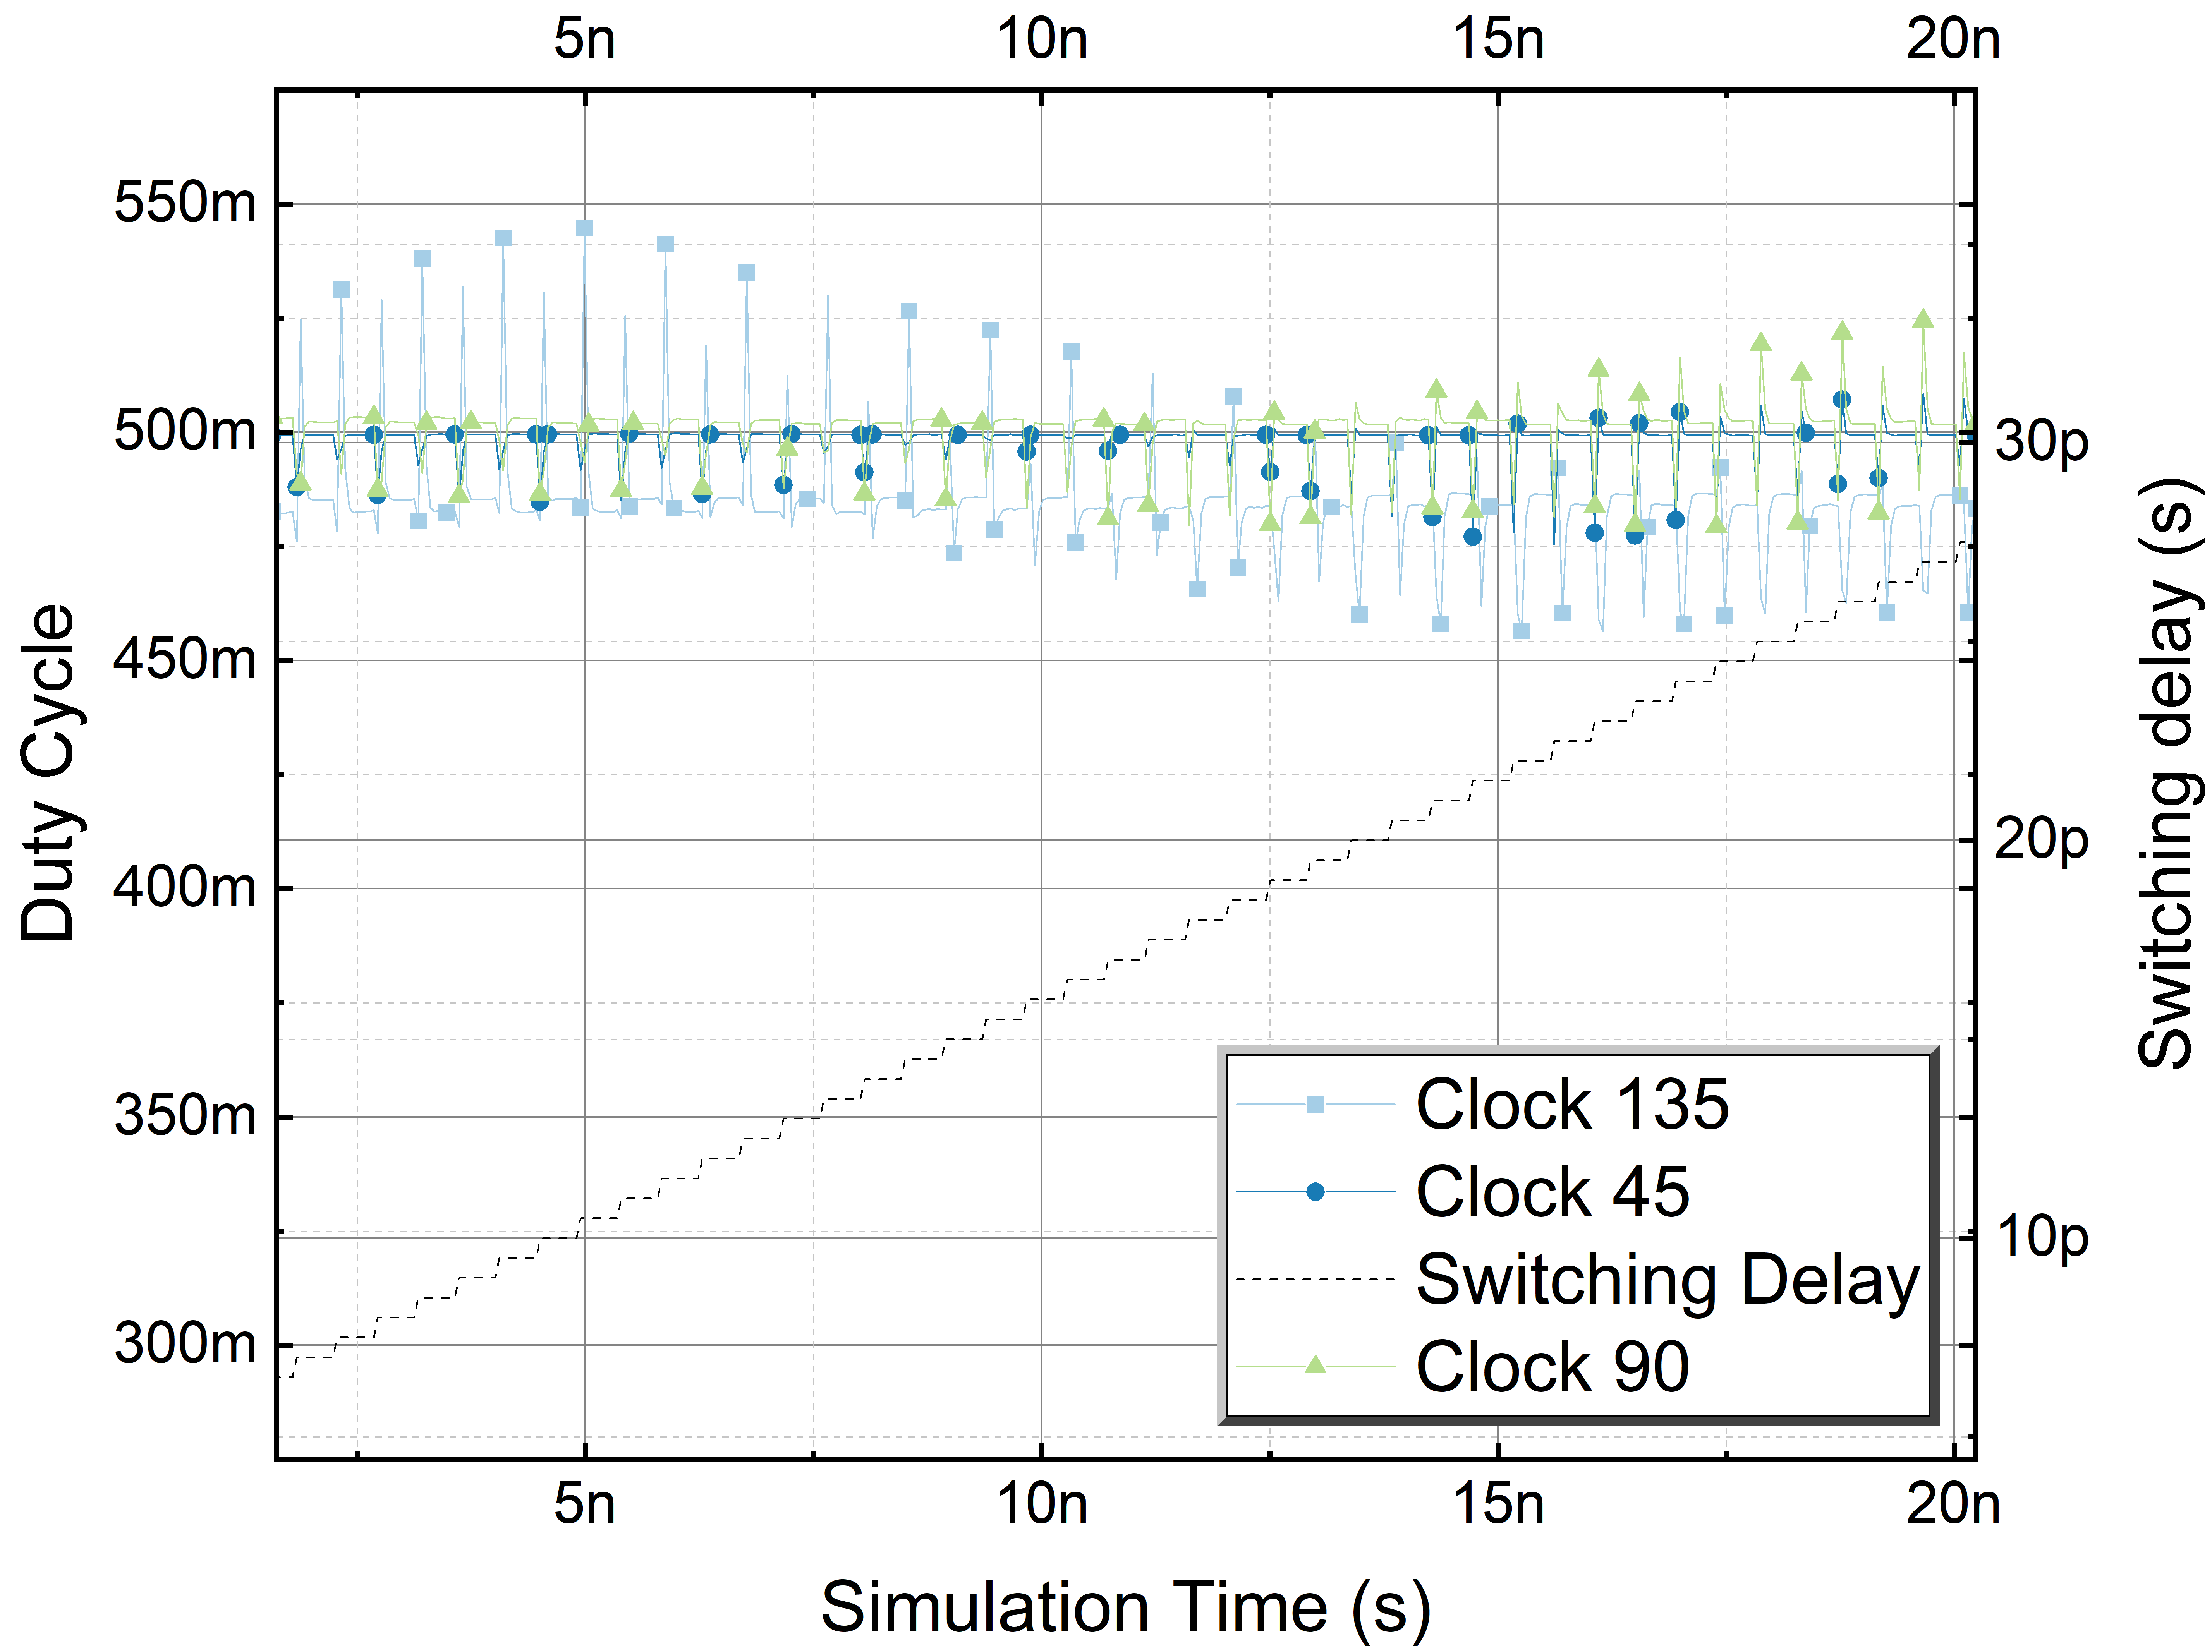
\includegraphics[width=0.8\linewidth]{figures/Results/Final_HF_LF_MF-DCD_vs_switchingDelay.png}
  \caption{Duty-cycle distortions as the MSB switches at different times across the clock period. The duty-cycle distortion is most significant at different times across branches.}
  \label{fig:dcd_MSB}
\end{figure}

\begin{figure}[H]
  \centering
  \hfill
  \begin{subfigure}[t]{0.3\linewidth}
    \centering
    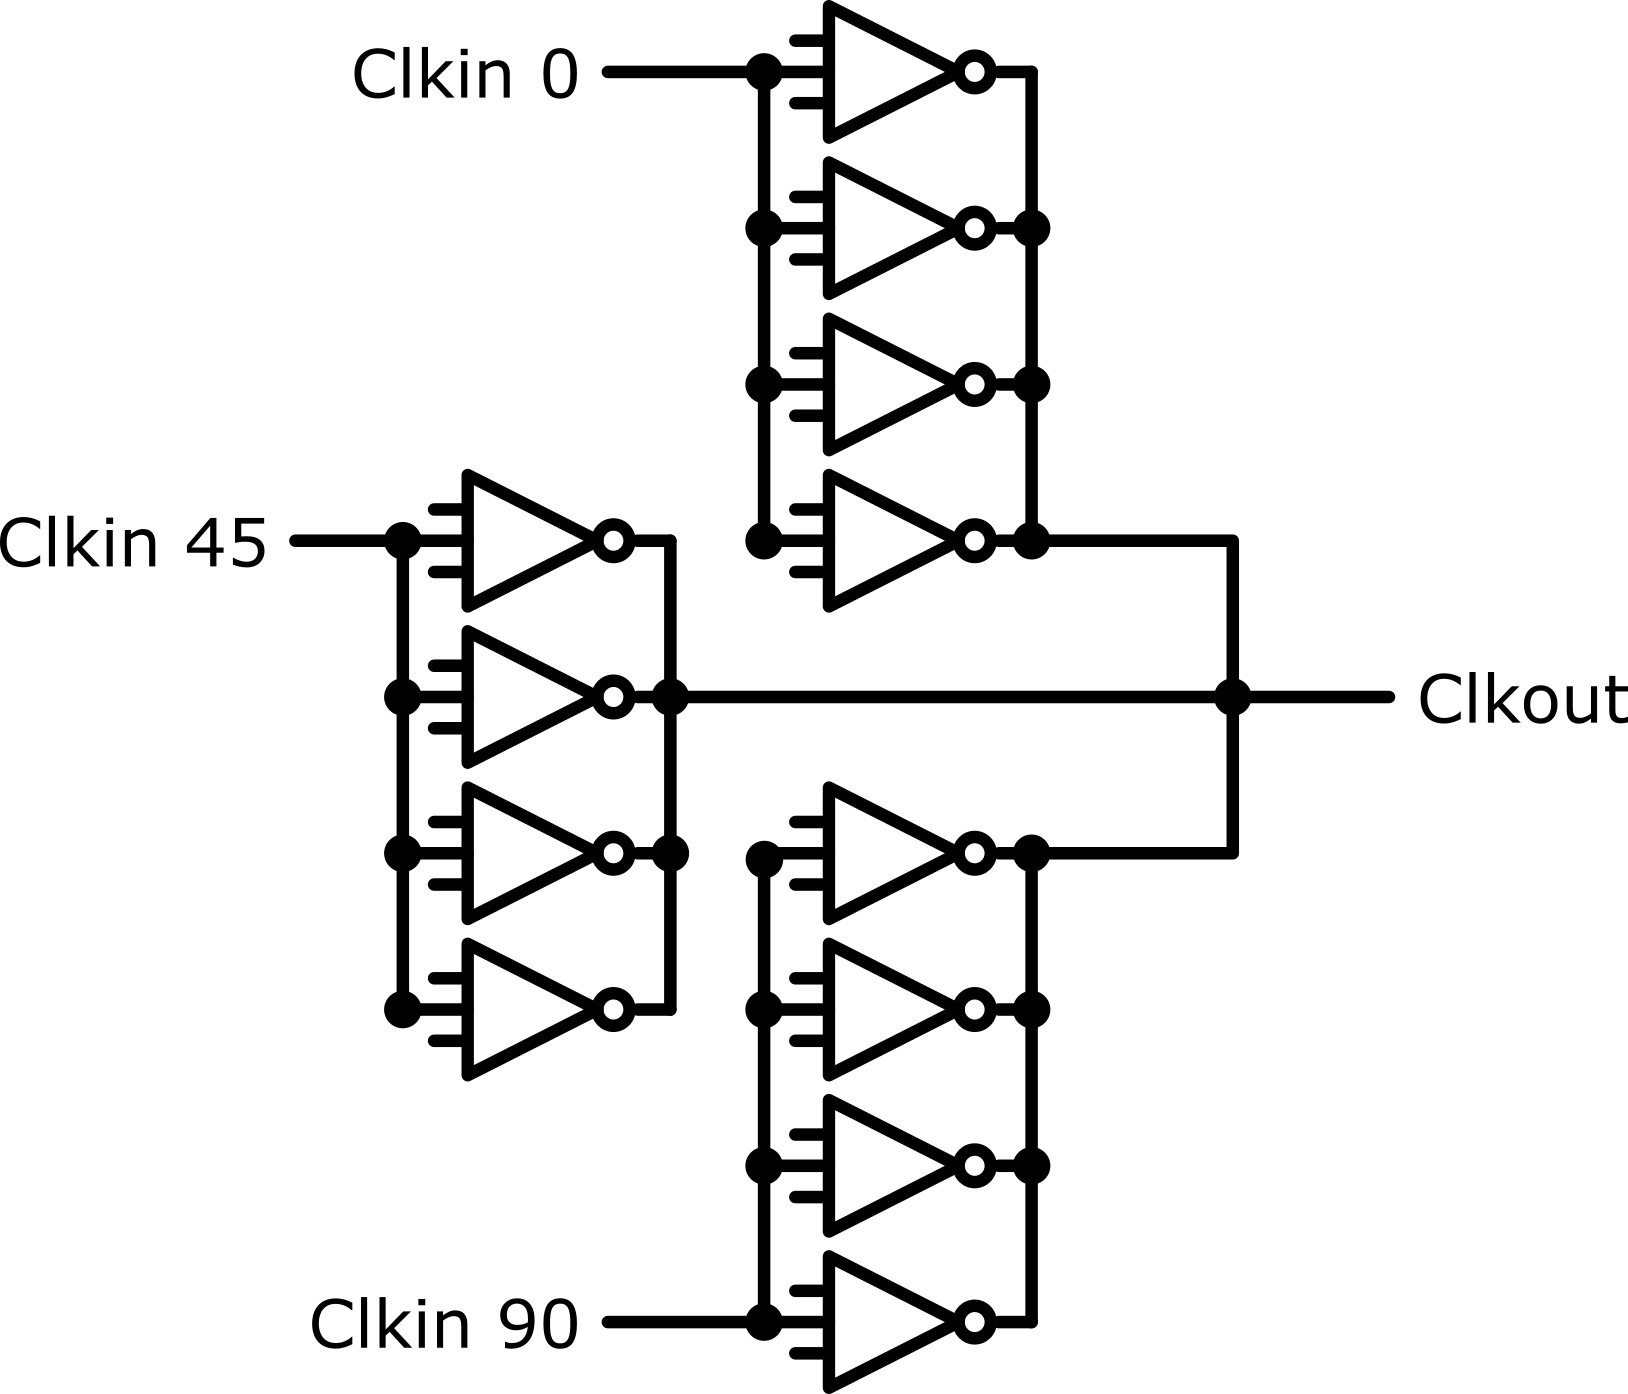
\includegraphics[width=\linewidth]{figures/Schematics/PhaseInterpolator_3paths.png}
    \caption{Phase interpolator with three clock paths (\ang{0}, \ang{90} and \ang{45}) driving tristate inverters.}
    \label{fig:phase_interpolator_3paths}
  \end{subfigure}%
  \hfill
  \begin{subfigure}[t]{0.3\linewidth}
    \centering
    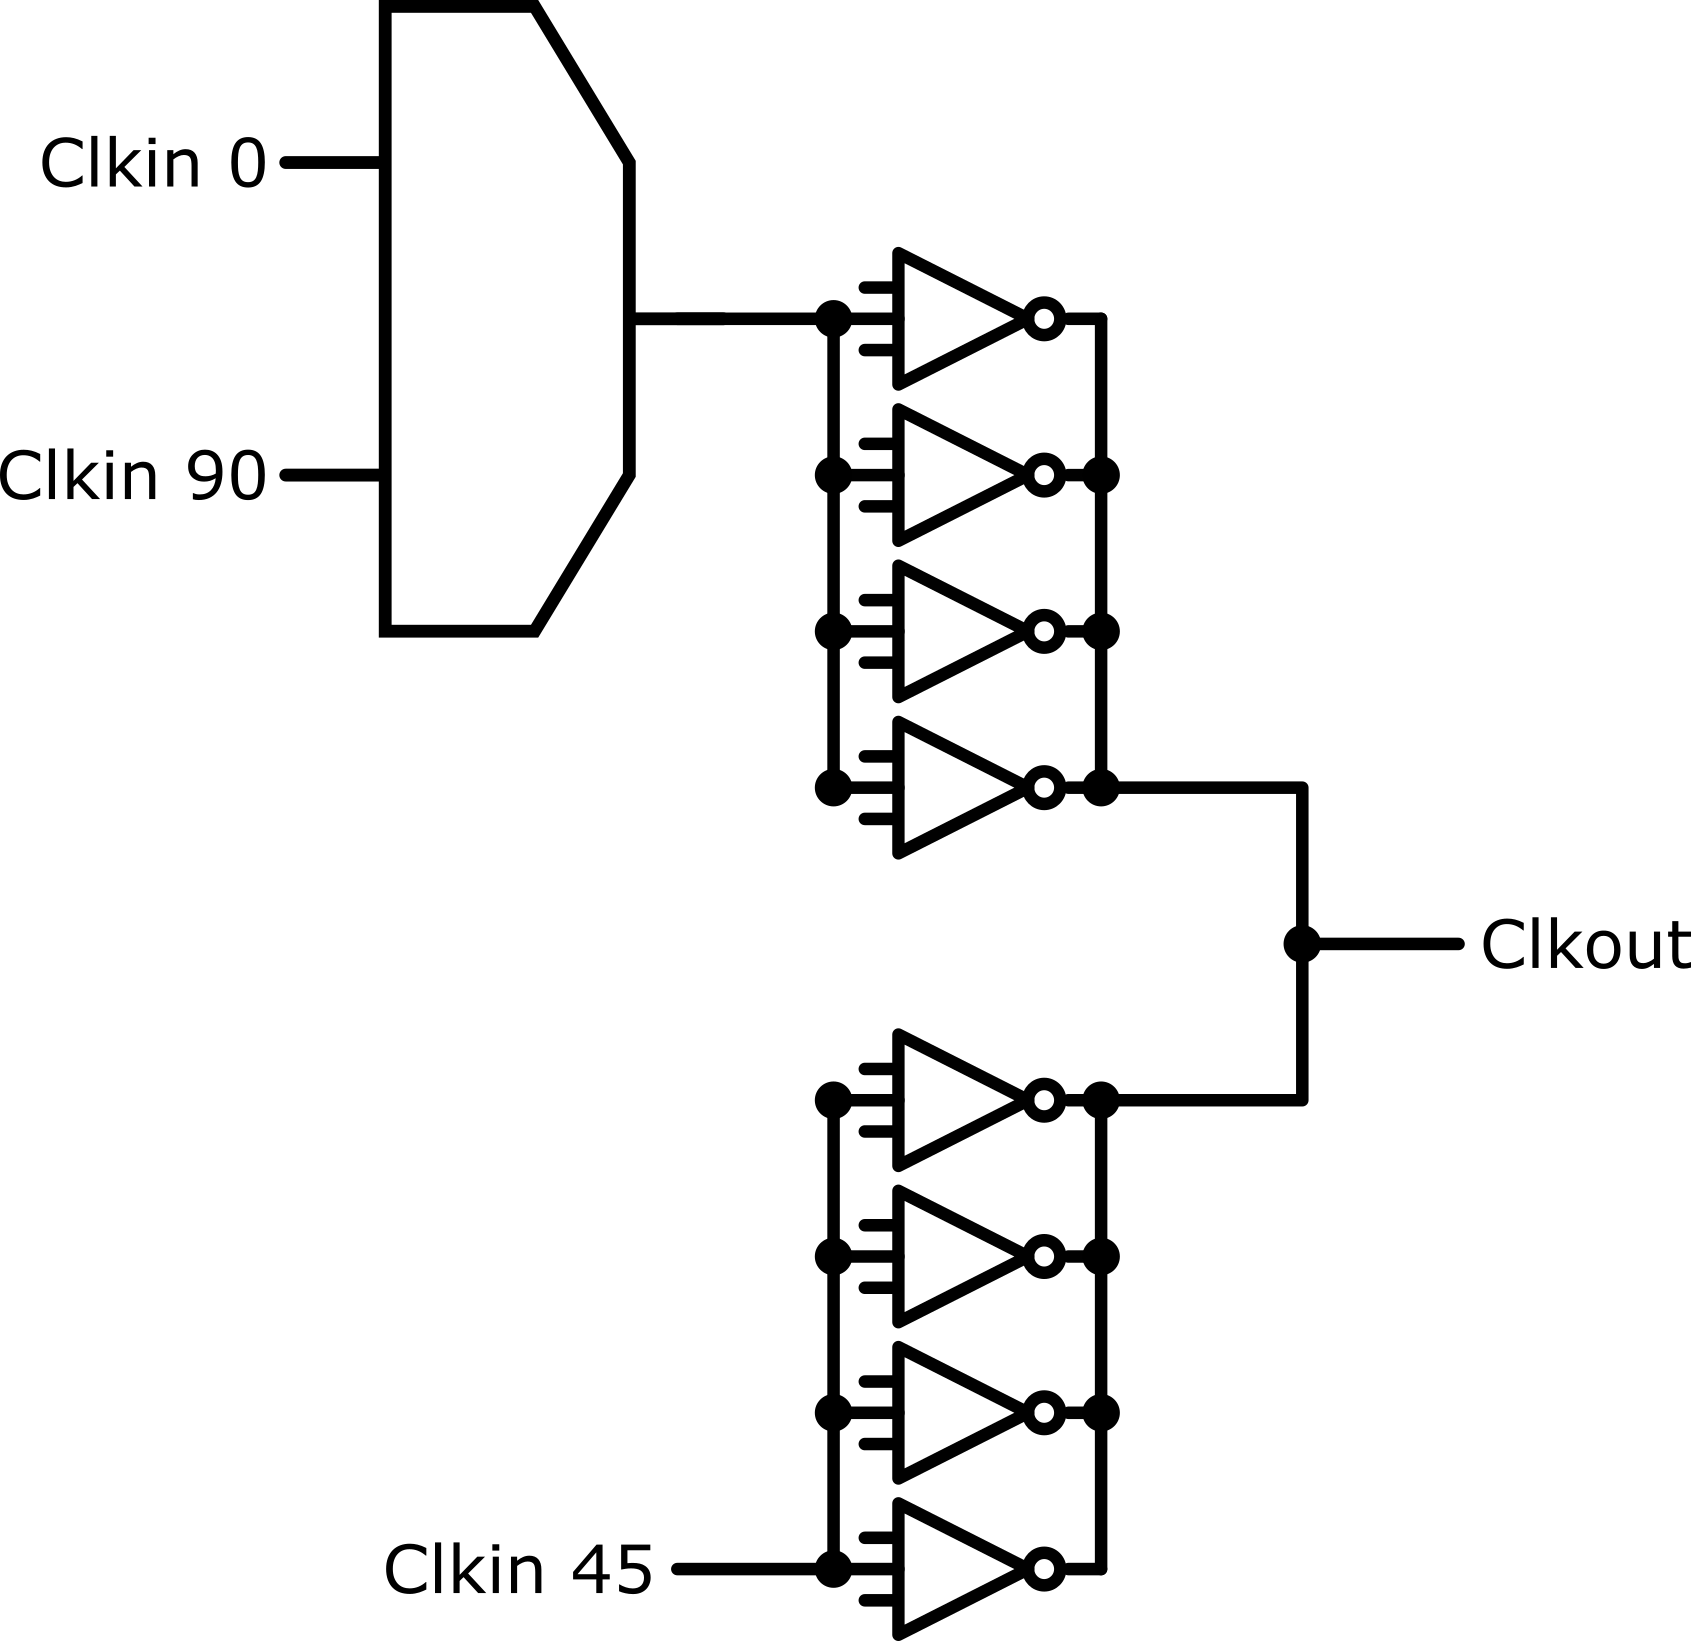
\includegraphics[width=\linewidth]{figures/Schematics/PhaseInterpolator_2paths.png}
    \caption{Phase interpolator with two clock paths (\ang{0} or \ang{90} and \ang{45}) driving tristate inverters.}
    \label{fig:phase_interpolator_2paths}
  \end{subfigure}
  \hfill\null
  \caption{Digitally-controlled phase interpolators for fine-tuning output clock phases. The first design employs three distinct clock paths, while the second design employs two inverter banks.}
  \label{fig:phase_interpolators}
\end{figure}


\subsection{Key Metrics}\label{final_key_metrics}

The final design of the multiphase generator was evaluated across various process corners and frequencies, achieving promising results. 

Jitter performance was measured at 22.5GHz, with the final design achieving an end-to-end jitter below 35~fs (Figure~\ref{fig:final_jitter}), accounting for the jitter introduced by the input demultiplexer, the multiphase generator, and the output multiplexer along with two stages of (at this stage parked) fine-tuning CSIs.

The final capacitor codes were verified to leave upper and lower margin of around 5 codes over PVT (Figure~\ref{fig:final_codes}). This may be insufficient for monte carlo drifts, but more range can be easily added by either increasing the number of bits in the capacitance banks or by increasing the step size.

Power consumption was measured at all operating modes using 22.5~GHz input clocks, with the final design consuming approximately 60mW in HF mode, 40mW in MF mode and 15mW in LF mode. Stacked column charts in Figure~\ref{fig:power_consumption} show the power consumption breakdown across the different components of the design. The sole contributor to the power consumption in HF is naturally the multiphase generator, while in MF the clock divider and the multiphase generator contribute almost equally to the power consumption. In LF mode, the clock divider is the main contributor to power consumption, while all other power consumption is negligible and very likely coming from small leakage currents and small clock feed-through disturbances.

\begin{figure}[H]
  \centering
  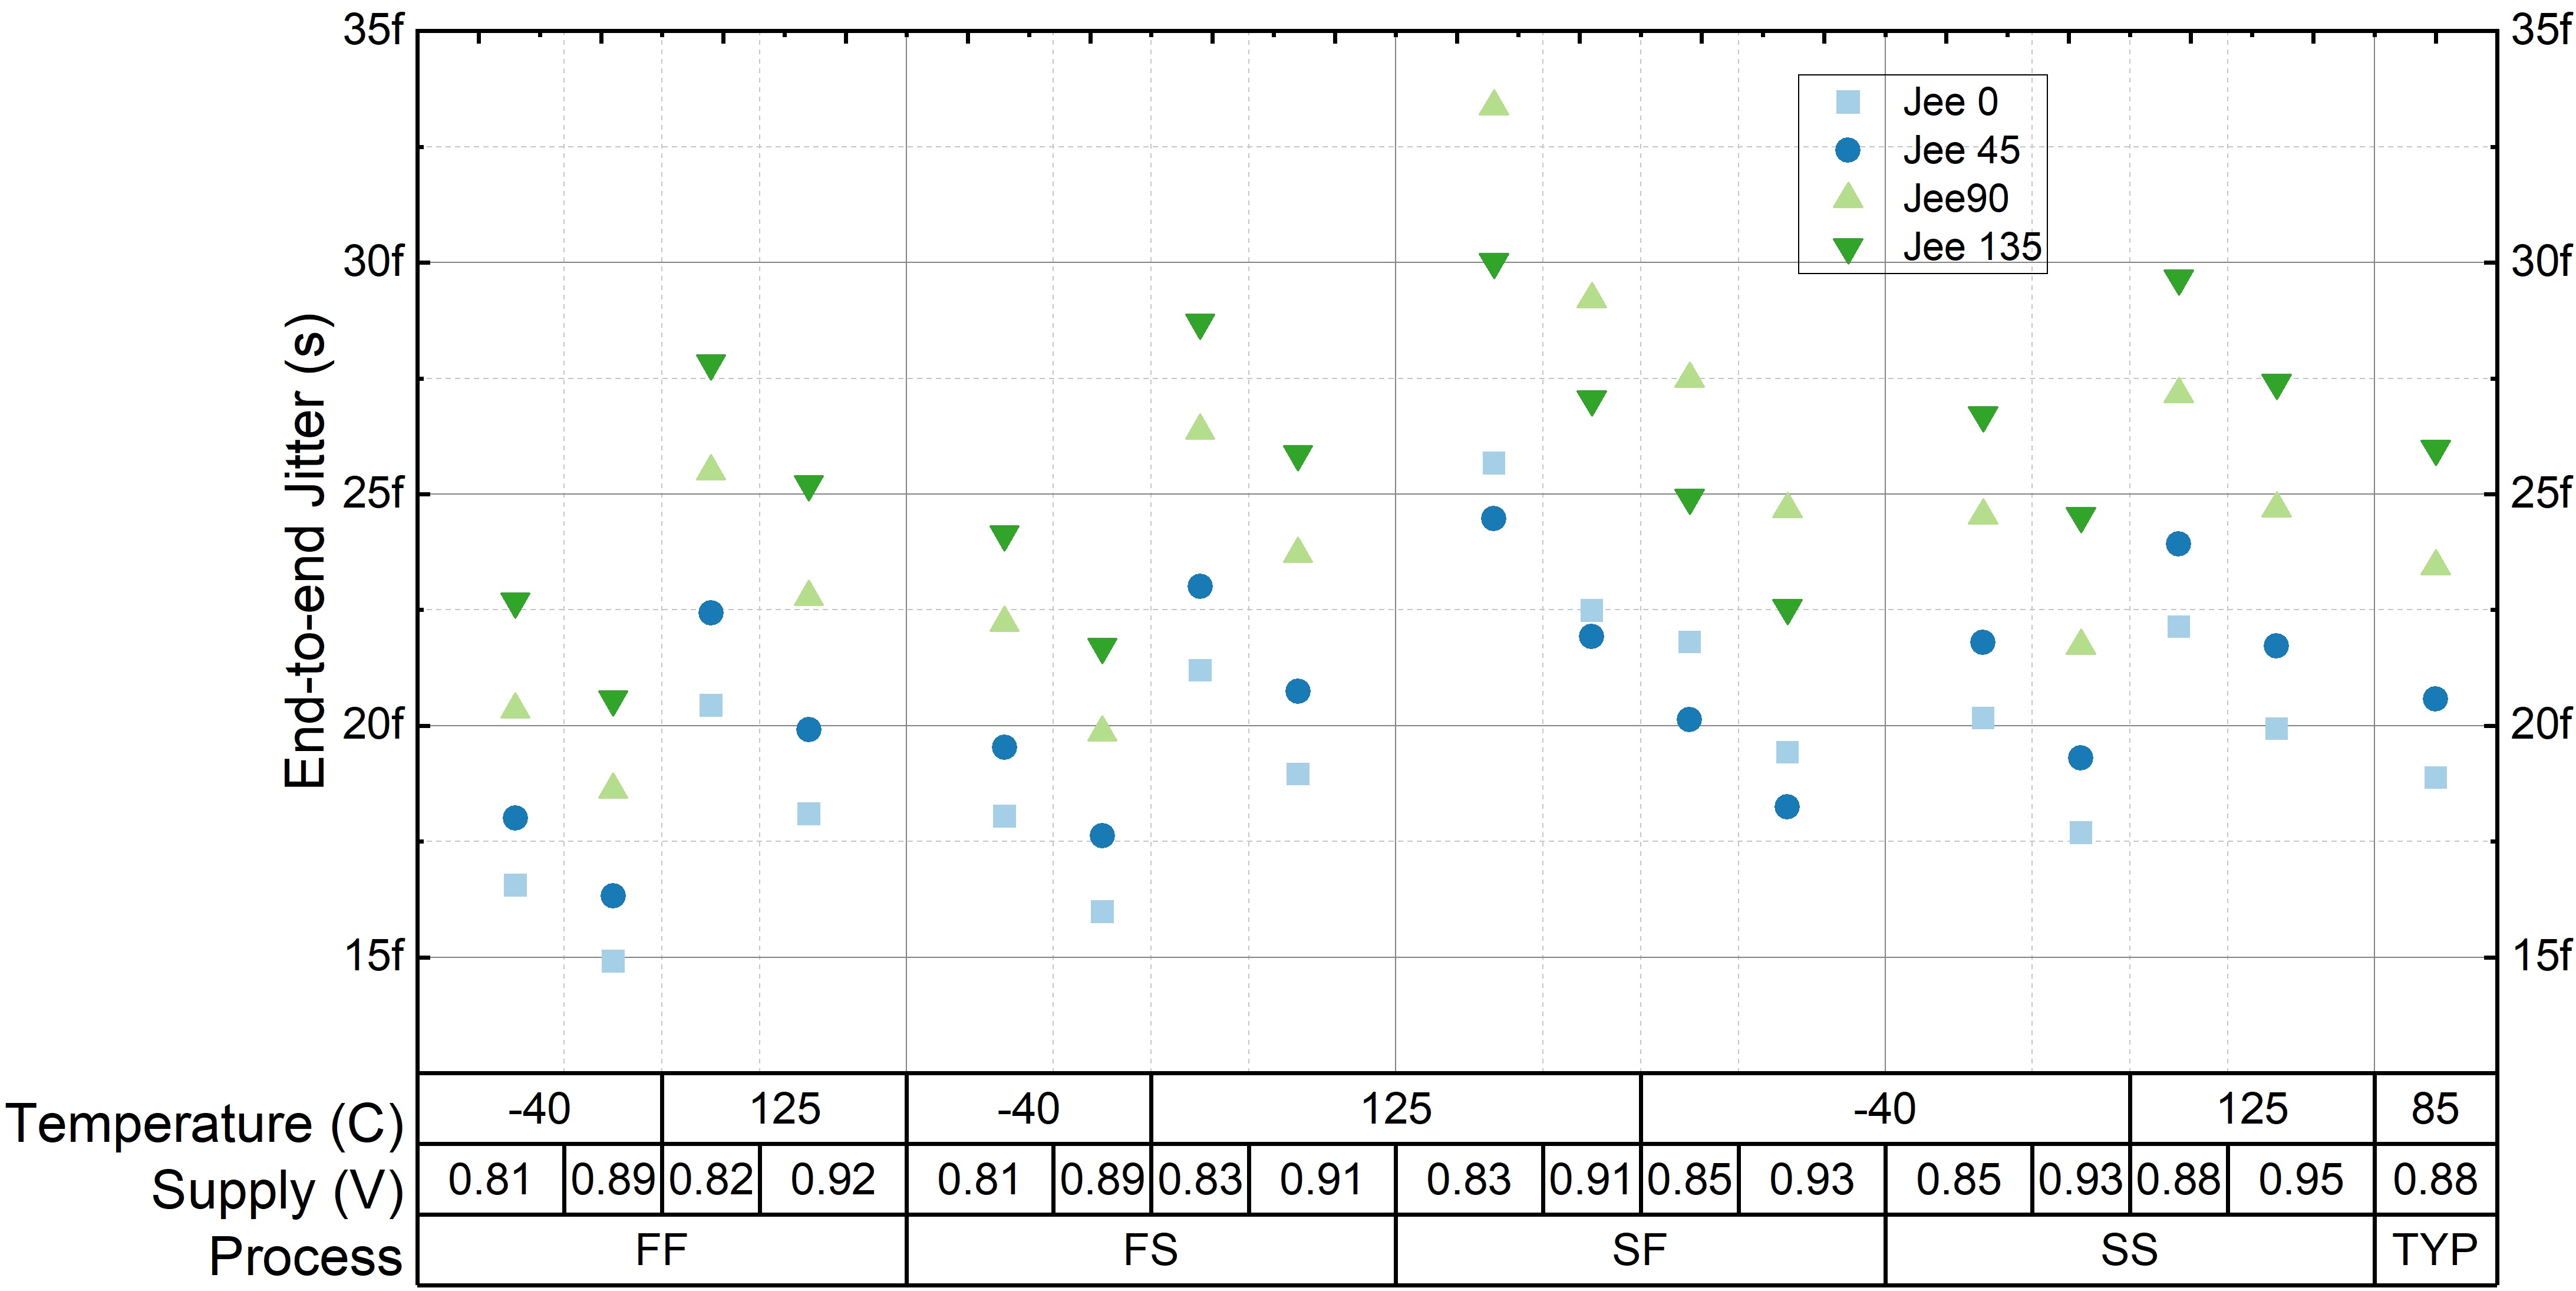
\includegraphics[width=0.8\linewidth]{figures/Results/Final_HF_LF_MF-Pivot_Jee.png}
  \caption{End-to-end jitter performance of the final multiphase generator design at 22.5GHz, achieving a jitter below 35fs across PVT corners.}
  \label{fig:final_jitter}
\end{figure}

\begin{figure}[H]
  \centering
  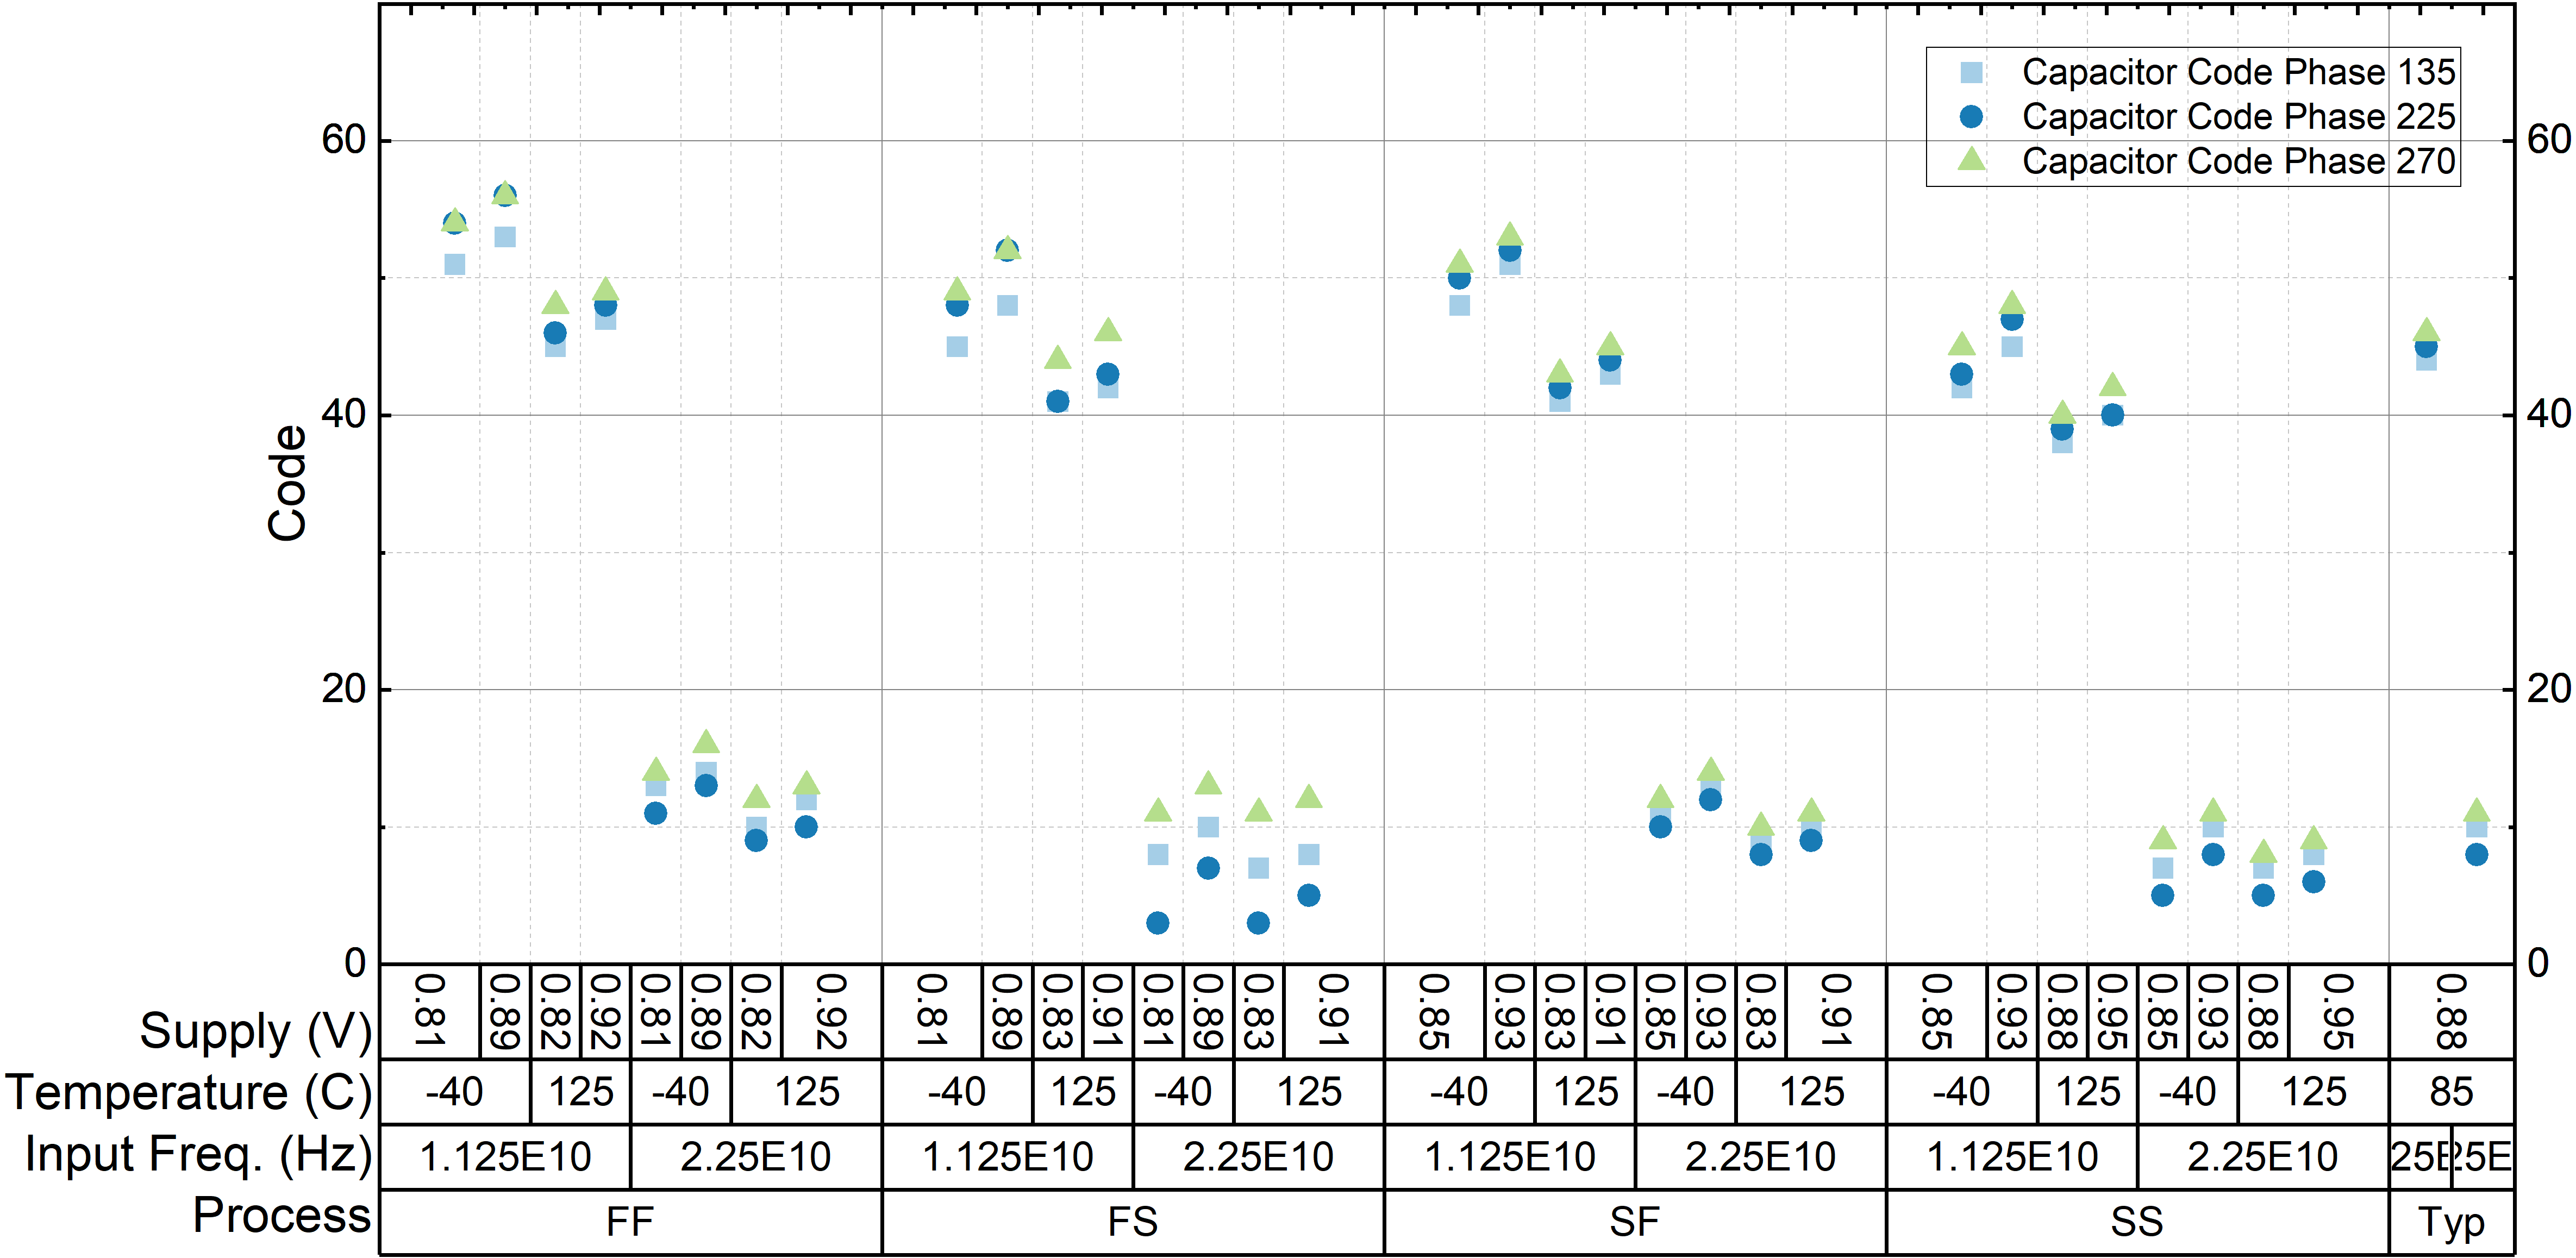
\includegraphics[width=0.8\linewidth]{figures/Results/Final_HF_LF_MF-Pivot_CapCodes_HF.png}
  \caption{Final capacitor codes across PVT corners, showing code margins in both directions. The codes are verified to be sufficient for PVT correction.}
  \label{fig:final_codes}
\end{figure}

\begin{figure}[H]
  \centering
  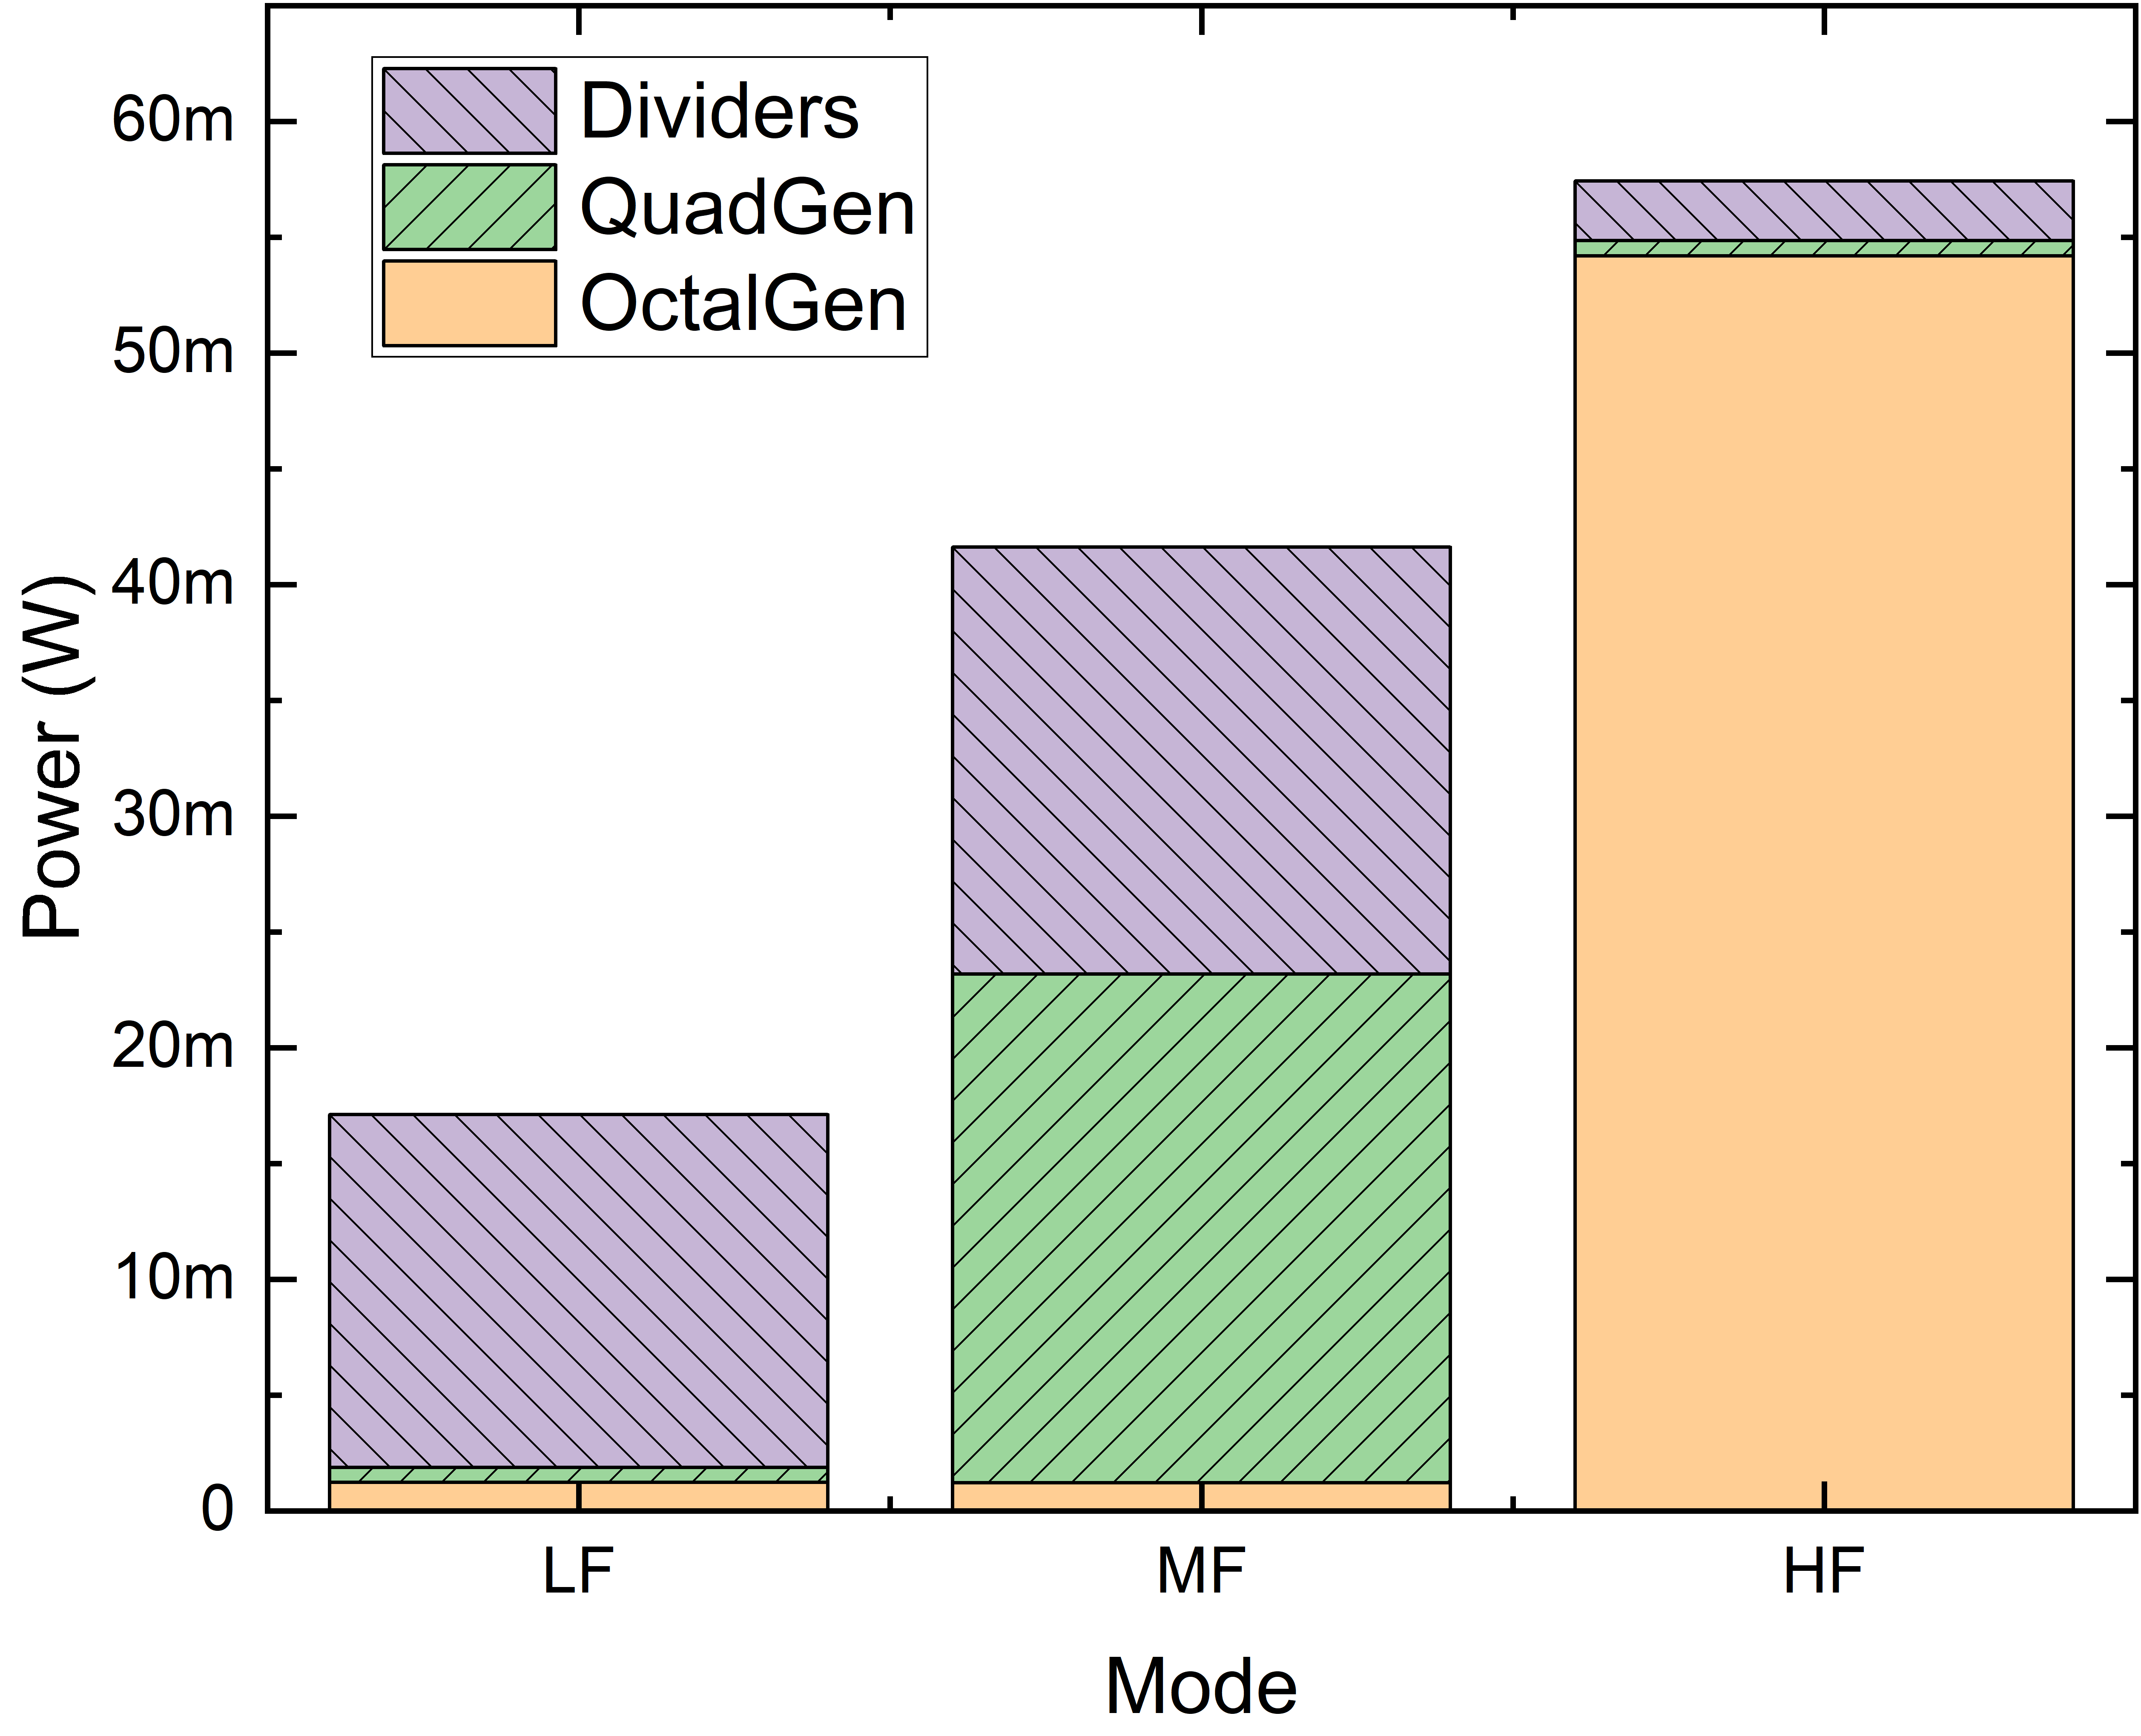
\includegraphics[width=0.8\linewidth]{figures/Results/Final_HF_LF_MF-power_distributions_LFMFHF.png}
  \caption{Power consumption breakdown of the final multiphase generator design across different modes of operation. The charts show the power consumption contributions of the multiphase QuadGen, OctalGen and clock divider, in high-frequency (HF), mid-frequency (MF), and low-frequency (LF) modes.}
  \label{fig:power_consumption}
\end{figure}

Overall, the final multiphase generator design demonstrates robust performance across a wide range of frequencies and process corners, achieving low jitter, efficient power consumption, and reliable operation in all three modes (HF, MF, LF). The design is well-suited for high-speed clock generation applications in advanced CMOS technologies, providing a versatile solution for generating multiple clock phases with dynamic tuning capabilities.